\documentclass[sigconf]{acmart}

\settopmatter{printacmref=false} % Removes citation information below abstract
\renewcommand\footnotetextcopyrightpermission[1]{} % removes footnote with conference information in first column
\pagestyle{plain} % removes running headers

\usepackage{subfig}
\usepackage{algorithm}
\usepackage{algorithmic}
\usepackage{multirow}
\usepackage{colortbl}
\usepackage[most]{tcolorbox}
\usepackage{dblfloatfix}
\usepackage{pifont}
\usepackage{tikz}
\usepackage{pgfplots}
\usepackage{enumitem}
%\usepackage{subfigure}
\usepackage{wasysym}
\usepackage{xspace}
\usetikzlibrary{backgrounds, positioning, fit}
\usetikzlibrary{shapes.geometric}
\usepackage{amsmath}
\usetikzlibrary{patterns}
\usetikzlibrary{pgfplots.groupplots}
\newcommand{\ballnumber}[1]{\tikz[baseline=(myanchor.base)] \node[circle,fill=.,inner sep=1pt] (myanchor) {\color{-.}\bfseries\footnotesize #1};}
\newcommand{\method}{{\scshape Gecko}}
%\newcommand{\method}{{\textsc{Gecko}\xspace}}
\newcommand{\cmark}{\CIRCLE}
\newcommand{\xmark}{\Circle}
\newcommand{\smark}{\LEFTcircle}


\begin{filecontents}{comparedef.txt}
z   n   pFA pFB
10  FP   98.16   86.16
10  AdvReg   87.48   83.66
10  DP   92.80   85.11
10  Gecko   90.49   83.52
20  {}  0   0
20  FP   97.86   80.34
20  AdvReg   73.97  71.02
20  DP   84.76  79.27
20  Gecko   76.79  73.5
30  {}  0   0
30  DP   99.58  88.95
30  AdvReg   89.09  85.19
30  DP   90.46  84.91
30  Gecko   93.45  85.8
\end{filecontents}

\begin{document}

\title{GECKO: Reconciling Privacy, Accuracy and Efficiency in Embedded Deep Learning}

\author{.}
%\author{Vasisht Duddu$^1$, Virat Shejwalkar$^2$, Antoine Boutet$^1$}
%\affiliation{\institution{$^1$ \large Univ Lyon, INSA Lyon, Inria, CITI \\ $^2$ \large University of Massachusetts Amherst}}
%\email{vduddu@tutamail.com, vshejwalkar@cs.umass.edu, antoine.boutet@insa-lyon.fr}


\begin{abstract}

Embedded systems demand on-device processing of data using Neural Networks (NNs) while conforming to the memory, power and computation constraints, leading to an efficiency and accuracy tradeoff. To bring NNs to edge devices, several optimizations such as model compression through pruning, quantization, and off-the-shelf architectures with efficient design have been extensively adopted. These algorithms when deployed to real world sensitive applications, requires to resist inference attacks to protect privacy of user’s training data. However, resistance against inference attacks is not accounted for designing NN models for embedded systems. In this work, we analyse the three-dimensional privacy-accuracy-efficiency tradeoff in NNs for embedded systems and propose Gecko training methodology where we explicitly add resistance to private inferences as a design objective. We use the inference-time memory, computation and power constraints of embedded devices as a criterion for designing NN architecture while preserving privacy. We choose quantization as design choice for highly efficient and private models. This choice is driven by the observation that compressed models leak more information compared to baseline models while off-the-shelf efficient architectures indicate poor efficiency and privacy tradeoff. We show that models trained using Gecko methodology are comparable to prior defences against blackbox membership attacks in terms of accuracy and privacy while providing efficiency.


%Embedded systems demand on-device processing of data using Neural Networks while conforming to the memory, power and computation constraints, leading to an efficiency and accuracy tradeoff.
%In order to bring Neural Networks to edge devices, several state of the art optimizations such as model compression through \textit{pruning}, \textit{quantization}, and \textit{off-the-shelf architectures} with efficient design have been extensively adopted.
%These algorithms when deployed to real world sensitive applications, such as healthcare monitoring wearables, requires to resist inference attacks to protect privacy of user's training data.
%However, resistance against inference attacks is not accounted for designing NN models for embedded systems.
%In this work, we analyse the three-dimensional \textit{privacy-accuracy-efficiency} tradeoff in Neural Networks for embedded systems and propose \method\hspace{0.02in} training methodology where we explicitly add resistance to private inferences as a design objective of Neural Networks.
%We use the inference-time memory, computation and power constraints of embedded devices as a criterion for designing Neural Network architecture while preserving privacy (captured through membership inference attack where the adversary aims to infer whether a given data point was a member of the model's training data or not).
%Given the flexibility of modifying a model during training, we choose quantization as our design choice for highly efficient and private models.
%This choice is driven by the observation that compressed models leak more information compared to baseline models while off-the-shelf efficient architectures indicate poor efficiency and privacy trade-off.
%We show that models trained using \method\hspace{0.02in} methodology are comparable to prior state of the art defences against blackbox membership inference attacks in terms of test accuracy and privacy while additionally providing efficiency.
\end{abstract}
\keywords{Membership Privacy, Inference Attacks, Efficient Deep Learning, Embedded Computing.}

\maketitle


\section{Introduction}\label{introduction}

The tremendous performance of Machine Learning, especially Deep Learning, models has resulted in their deployment to low-powered edge devices and embedded systems.
Specifically, Internet of Things (IoT) devices extensively prefer on-device processing to reduce communication latency and overhead, while also preserving the privacy of data from an untrusted data curator~\cite{8110880}.
The design of efficient Neural Networks (NNs) requires algorithm-hardware co-design such as model compression, quantization, and designing special architectures with higher efficiency~\cite{8114708}.
% that are extensively used for industry applications
Such NN architecture design optimizations should conform to efficiency constraints on memory, energy, and computation overhead on embedded devices, and also maintain high prediction accuracy.
However, such designs often result in \textit{efficiency-accuracy} trade-off~\cite{rastegari2016xnornet}.

Additionally, privacy laws, such as HIPAA and GDPR, require on-device processing to maintain the privacy of user's sensitive data (e.g, medical records, location traces, and purchase preferences).
In this work we focus on Membership Inference Attack~\cite{shokri2017membership}, where given a target model and a target record, the adversary determines if the target data record was part of the target model's training data by analyzing the target model's output predictions.
For instance, wearable devices, which monitor its user's health, commonly rely on NNs for various health related predicts. Such devices are continuously trained on the private data of a large number of users, and therefore, by mounting membership inference attacks on target device, an adversary can determine if the data of a target user was used to train NNs on the target device.
In such cases, it is crucial to design NNs resistant to inference attacks, where the adversary infers unobservable, sensitive information (e.g, user's health status) from the observable information (e.g., model predictions).
We refer to computations that achieve privacy through inference-resistance as {\em privacy-preserving computation}.
%Multiple works propose privacy preserving mechanisms to address the issue of privacy leakage
Such privacy preserving computation mechanisms affect the model's predictive accuracy resulting in \textit{privacy-accuracy} trade-off~\cite{Abadi:2016:DLD:2976749.2978318,DBLP:conf/ccs/NasrSH18,shejwalkar2019reconciling}.

Considering the trade-offs described above, the three objectives to consider while designing NNs for embedded devices are: (a) high prediction accuracy, (b) efficiency constraints on memory, energy, and computation overhead, and (c) preserving privacy of on-device data.
However, designing a model to preserve privacy while satisfying efficiency requirements without a significant cost of the model’s predictive accuracy is challenging.
%Designing NNs that meet all of the above objectives is a significantly challenging task due to the aforementioned trade-offs.
%In this work, we address the research question: \textit{How can we redesign NNs to reconcile privacy and efficiency in Deep NNs without a significant loss in accuracy?}

In this paper, we address this challenge by proposing \method\hspace{0.02in} — a two phase training methodology for designing NNs optimized specifically for performance, accuracy and privacy. We evaluate the privacy leakage of three state of the art hardware software co-design techniques, namely, model compression, quantization and efficient off-the shelf architectures. We show that model compression leaks more information compared to baseline (uncompressed) models indicating a higher privacy risk to the user’s data while off-the-shelf architectures (MobileNet and SqueezeNet) do not meet all the efficiency requirements but can provide limited privacy leakage. These observations motivate our design choice of quantizing NNs as part of \method\hspace{0.02in} training algorithm.

%In this paper, we first highlight the three-way trade-off between accuracy, efficiency, and privacy due to NNs designed for embedded devices.
%More specifically, we evaluate membership privacy leakage due to the three state-of-the-art hardware-software co-design techniques: model compression, quantization, and efficient off-the shelf architectures.
%We show that model compression leaks more information compared to the baseline (uncompressed) models and poses higher privacy risks to the user's data.\virat{add some numbers here}
%\red{Off-the-shelf architectures (e.g., MobileNet and SqueezeNet) do not meet all the efficiency requirements but can provide more limited privacy leakage.}\virat{clarify using numbers}
%These observations motivate our design choice of quantizing NNs as part of \method\hspace{0.02in} training algorithm.
%It is worth noting that, previous works have explored the the efficiency-accuracy~\cite{rastegari2016xnornet} and privacy-accuracy~\cite{shokri2017membership} trade-offs, however separately. To address the above shortcoming, 

% \noindent\textbf{Our contributions:} In this paper, we address this challenge by proposing %provide directions to design NNs for efficiency private inference.
% %We present 
% \method~ --- a two phase training methodology to design NNs optimized specifically for accuracy, efficiency, and privacy.
% We evaluate the privacy leakage of three state of the art hardware software co-design techniques, namely, model compression, quantization and efficient off-the shelf architectures.
% We show that model compression leaks more information compared to baseline (uncompressed) models indicating a higher privacy risk to the user's data while off-the-shelf architectures (MobileNet and SqueezeNet) do not meet all the efficiency requirements but can provide more limited privacy leakage.
% %acceptable 
% % this term should be avoided (what is acceptable?)
% These observations motivate our design choice of quantizing NNs as part of \method\hspace{0.02in} training algorithm.

%we propose \method\textemdash a two phased training methodology to design NNs optimized specifically for accuracy, efficiency, and privacy. 
In Phase-I of \method, the model parameters and activations are binarized, i.e., constrained to \{-1,+1\} to reduce the memory, energy consumption, and computation overhead.
To ensure computation efficiency, we replace the expensive multiply accumulate operations between parameter matrices and activation vectors 
% from previous layers 
to simple and cheaper XNOR operations.
As our main contribution, we show that aggressively quantized NN architectures obtained in Phase-I ensure efficient privacy-preserving computation with higher resistance to membership inference attacks.%\red{why is it better?}
Phase-I of \method\hspace{0.02in} optimizes for efficiency \textit{and} privacy but at the cost of a significant drop in accuracy.
In Phase-II, we restore this accuracy 
%to acceptable standard compared to the original (full precision model) accuracy
by transferring knowledge from larger full precision models to the quantized models~\cite{shejwalkar2019reconciling}.
Here, the quantized XNOR model uses the output predictions of the full precision state of the art models as labels instead of using the true labels during training.
This results in significantly increase in the prediction accuracy of the model while limiting privacy leakage. 
%with a small but acceptable increase in privacy leakage.

%In summary, \method\hspace{0.02in} training algorithm comprises of Phase I of \textit{Quantizing} to reduce the precision of model with binary values with XNOR computations which provides efficiency and privacy.
%This is followed by Phase II of \textit{Distillation} to restore the accuracy degradation by transferring the knowledge learnt from the full precision to the efficient quantized model.

Finally, we compare the models trained using \method\hspace{0.02in} with prior state-of-the-art defences against membership inference attacks, namely, Adversarial Regularization~\cite{DBLP:conf/ccs/NasrSH18} and Differential Privacy~\cite{Abadi:2016:DLD:2976749.2978318}.
We show that our proposed models improve the trade-offs between the efficiency,  accuracy, and privacy compared to the baselines approaches. Our work provides the first systematic evaluation efficiency-accuracy-privacy trade-offs to design a novel training methodology. The code is made publicly available\footnote{Anonymized for Submission}.
%, and show that our proposed models performance is comparable to the state of the art.
%However, our models provide an additional guarantee of higher efficiency which models trained with prior defences fail to provide.

The paper is outlined as follows: Section~\ref{background} presents background in embedded Deep Learning while Section~\ref{analysis} reports a comparative analysis of state of the art baselines.
We describe \method\hspace{0.02in} in Section~\ref{design} and evaluate it Section~\ref{compare}. Related work are then presented Section~\ref{related} before concluding in Section ~\ref{conclusions}.

%The paper is outlined as follows: We describe the threat model and describe the state of the art algorithms for embedded Deep Learning in Section~\ref{background} followed by identifying the best optimization technique to satisfy privacy and efficiency in Section~\ref{motivate}. Based on the observations, we describe the Phase I and Phase II design of \method\hspace{0.02in} training algorithm in Section~\ref{design}.
%Finally, we show that the proposed optimization for NNs is comparable to prior state of the art privacy preserving defences (Section~\ref{compare}) while additionally providing efficiency guarantees.

\section{Background}
\label{background}

\subsection{Embedded Deep Learning}

On-device processing is an attractive alternative compared to centralized processing of data from sensors, IoT and embedded edge devices.
Such on-device processing reduces the overhead of communicating data from the devices to the servers, lowers the privacy and security risk associated with storing sensitive data on untrusted central server and lowers the latency for obtaining results from processing~\cite{8110880}.

Different efficiency requirements can be adopted to design NNs for embedded systems.
These differences make it difficult to decide which primitive is the best fit for designing a privacy-preserving system for a particular application.
The list below presents the most important efficiency requirements accounted by designers of embedded systems using NNs, and privacy is not part of this list:

\begin{itemize}[leftmargin=*]
\item {\em Energy Efficiency.} Energy consumption is a vital constraint for low powered embedded or IoT devices which operate for long duration while maximising their battery lifetime.
While executing NNs, every Multiply Accumulate (MAC, a common step that computes the product of two numbers and adds that product to a register in which intermediate results are stored) requires memory access for reading weights, inputs and intermediate output from previous layer and one write to store the computed output which is significantly higher than actually performing the MAC operation in the CPU.
Energy efficiency is achieved by reducing the memory access by (a) optimizing hardware to exploit sparsity in MACs and (b) reducing the precision to increase the throughput of data.

\item {\em Computation Efficiency.} The total MAC operations between the parameter matrix and input activation function quantifies the requirement of computation efficiency.
The processing rate of MAC operations is constrained by the CPU on embedded device which is reduced by reducing the total number of parameters.
Additionally, replacing MACs with cheaper binary arithmetic significantly lowers the computational overhead.

\item {\em Memory Efficiency.} The total size of the model measured in terms of the memory storage for model parameters and additional runtime storage for intermediate outputs should be within the memory constraints of the embedded device.
This is achieved in two ways: (a) reducing the precision of the parameters and intermediate outputs and (b) pruning the parameters by increasing sparsity.
\end{itemize}


%In order to execute trained NN models on low powered edge devices, optimizations are required for the design of the NN architectures.
%Model designers use three state of the art approaches for designing efficient NN models for embedded systems: (a) Model Compression via Pruning, (b) quantization of model parameters and activations and (c) designing standard architectures (off the shelf efficient architectures).
%%In this work, we consider these three approaches as baselines for comparison and evaluation to select the choice of optimization for \method.

%\begin{itemize}[leftmargin=*]
%\item {\em Model Compression (Pruning).} 
%NNs are overparameterized, i.e, have large number of redundant weights.
%Pruning of the network refers to removing these redundant weights (setting them as zero) without a degradation of model accuracy.
%The pruning operation results in a model with sparse parameters for which the hardware can be designed to skip the multiplication and memory storage, improving the efficiency.
%Sparse weights can be stored in a compressed format in the hardware using the compressed sparse row or column format which reduces the overall memory bandwidth~\cite{DBLP:journals/corr/HanMD15,10.1109/ISCA.2016.30,Han:2015:LBW:2969239.2969366}.
%Aggressive pruning, while compresses the model significantly, requires to be re-trained to restore the model's original accuracy.
%For a threshold $T$, the parameters close to zero are replaced by zero which is given as:
%\[
%\footnotesize
%    f(W)=
%\begin{cases}
%    0, & \text{if } -T \leq w \leq T\\
%    w,  & \text{otherwise}
%\end{cases}
%\]

%\item {\em Off-the-Shelf Efficient Architectures.} 
%NNs can be redesigned by changing the hyperparameters (filter size in convolution, number of layers and their types) to reduce the number of parameters and hence, the memory footprint.
%One approach is to replace larger convolution filters with multiple smaller filters with less number of parameters but covering the same receptive fields.
%For instance, one 5x5 filter can be replaced by two 3x3 filters.
%Alternatively, 1x1 convolutional layers reduce the number of channels in output feature map, lowering the computation and number of parameters.
%For instance, for an input activation of dimension 1x1x64, 32 1x1 convolutional filters downsamples the activation maps to get an output of 32 channels.
%Such optimizations enable to design compact network architecture with layers having lower parameters compared to the original model, extensively adopted in MobileNet~\cite{conf/cvpr/SandlerHZZC18} and SqueezeNet~\cite{DBLP:journals/corr/IandolaMAHDK16}.


%\item {\em Quantization.}
%Quantization reduces the precision of the model's parameters and the intermediate activations during execution.
%Quantization maps parameters and activations values to a fixed set of quantization levels~\cite{Hubara:2017:QNN:3122009.3242044}.
%The number of quantized levels determines the precision of the operands ($log_2(\#levels)$).
%Reducing the precision of the (a) parameters lowers the storage cost of the model in memory, (b) activations lowers the computation overhead by replacing MACs with binary arithmetic and (c) lowers the energy consumption by lowering the memory accesses and increasing throughput.
%Aggressively quantizing the parameters and activations to binary and ternary precision significantly improves the overall efficiency, however, at the cost of accuracy~\cite{rastegari2016xnornet}.
%For instance, Binarized NNs quantize the operands to \{-1,+1\} values~\cite{NIPS2016_6573} while ternary NNs have values \{-w, 0, w\} where $w$ can be fixed or learnt during training~\cite{Li2016TernaryWN}. These are examples of uniform quantization.
%Alternatively, weight sharing maps several parameters to a single value reducing the number of unique parameters.
%This mapping is done using K-Means clustering or a hashing function and the corresponding shared values are read from a "codebook" which maps different parameters to its shared value.
%\end{itemize}




%\section{Threat Model}\label{threatmodel}

\subsection{Privacy Threat: Membership Attacks}
%Inference
\label{threatmodel}

% section to reduce

Although commonly not taken into account for the design of NNs for embedded systems, privacy threats still exist if personal and potentially sensitive data feed the system.
Indeed, an adversary learns aggregate information about the entire data population through the model which generalizes this information from the train dataset to an unseen test data.
This is desirable and quantified using the accuracy of the model.
On the other hand, if the adversary learns something specific about a user's data record used in the training dataset, we refer to such information as privacy leakage.
In other words, in context of machine learning, there is a privacy breach if the adversary learns unobservable information specific to an individual user's data record from observable information such as model's output predictions.
This inferred unobservable information about a user's record can be, for instance, the membership details of the record in the training set of the model, referred to as membership inference attacks.
Alternatively, an adversary can learn sensitive attributes about the user's data record which can be used to reconstruct the sensitive training dataset.
In this work, we specifically use membership inference attacks to quantify information leakage in machine learning models~\cite{shokri2017membership}.


Machine Learning algorithms learn a function $f:X \rightarrow Y$ mapping from the input space $X$ to the space of corresponding class labels $Y$.
This is modeled as an optimization where the objective is to find the parameters $\theta$ by minimizing the model's loss, $min_{\theta} L(f(x),y;\theta)$.
Machine learning models are more confident while predicting the class of already seen train data record compared to an unseen test data record.
Membership inference attacks exploits this difference in the model's confidence to classify a new data record as being a "Member" or "Non-Member" of the model's training data.
This is a binary decisional problem where the adversary classifies the membership of a given input $x$ using the model's output prediction  $f(x;\theta)$ to infer whether a given data record was used in the model's training data or not.
Formally, given a user's data record $x$ $\sim$ $P(X,Y)$, where $P(X,Y)$ is the data distribution from which the training data $D_{train}$ was sampled, the adversary estimates $P(x \in D_{train})$ using the model's prediction $f(x;W)$.
Empirically, the adversary identifies a threshold to estimate whether $x \in D_{train}$ which can also be learnt using a binary classifier.
In this work, we use the confidence score attack where the adversary obtains $f(x;W)$ and finds the maximum posterior and infers $x \in D_{train}$ if the maximum is greater than a threshold~\cite{salem2018ml,8429311}.
The attack is based on the observation that the maximal posterior of a member data record is higher (more confident) than a non-member data record of the training dataset.


In this threat model, we consider a blackbox setting where the adversary is assumed to have no knowledge about the target model.
Formally, given a target model $f()$, the adversary only sees the final model prediction $f(x;\theta)$.
The adversary does not know the architecture of $f()$ and the model parameters $\theta$.
This is a practical setting seen typically in Machine Learning as a Service (MLaaS) where the adversary submits an input query to the trained model on the Cloud via an API and receives the corresponding output.




%Indeed, on querying a trained model $f(x;\theta)$, the adversary learns aggregate information about the entire data population which the model generalizes from the train dataset to an unseen test data.
%This is desirable and quantified using the accuracy of the model.
%On the other hand, if the adversary learns something specific about a user's data record used in the training dataset, we refer to such information as privacy leakage.
%In other words, in context of machine learning, there is a privacy breach if the adversary learns unobservable information specific to an individual user's data record from observable information such as model's output predictions.
%This inferred unobservable information about a user's record can be, for instance, the membership details of the record in the training set of the model, referred to as membership inference attacks.
%Alternatively, an adversary can learn sensitive attributes about the user's data record which can be used to reconstruct the sensitive training dataset.
%In this work, we specifically use membership inference attacks to quantify information leakage in machine learning models.

%Machine learning models are more confident while predicting the class of already seen train data record compared to an unseen test data record.
%Membership inference attacks exploits this difference in the model's confidence to classify a new data record as being a "Member" or "Non-Member" of the model's training data.
%This is a binary decisional problem where the adversary classifies the membership of a given input $x$ using the model's output prediction $f(x;\theta)$.
%We describe the threat model and attack details below.

%\noindent\textbf{Adversary Knowledge.} We assume a blackbox setting where the adversary is assumed to have no knowledge about the target model.
%Formally, given a target model $f()$ which maps an input data record $x$ to its correct label $y$, the adversary only sees the final model prediction $f(x;\theta)$.
%The adversary does not know the architecture of $f()$ and the model parameters $\theta$.
%This is a practical setting seen typically in Machine Learning as a Service (MLaaS) where the adversary submits an input query to the trained model on the Cloud via an API and receives the corresponding output predictions.

%\noindent\textbf{Adversary Goal.} The goal of adversary in membership inference attack is to infer whether a given data record was used in the model's training data or not.
%Formally, given a user's data record $x$ $\sim$ $P(X,Y)$, where $P(X,Y)$ is the data distribution from which the training data $D_{train}$ was sampled, the adversary estimates $P(x \in D_{train})$ using the model's prediction $f(x;W)$.
%Empirically, the adversary identifies a threshold to estimate whether $x \in D_{train}$ which can also be learnt using a binary classifier.

%\noindent\textbf{Attack Methodology.} In this work, we use the confidence score attack where the adversary leverages the prediction entropy of the target model $f(x;W)$ to perform the membership inference attack [][].
%In particular, the adversary obtains $f(x;W)$ and finds the maximum posterior and infers $x \in D_{train}$ if the maximum is greater than a threshold.
%The attack is based on the observation that the maximal posterior of a member data record is higher (more confident) than a non-member data record of the training dataset.



%\subsection{Metrics}

%We use the inference attack accuracy to estimate the success of membership inference attack.
%An accuracy above random guess $50\%$ indicates a training data leakage through membership inference attack.
%This indicates that the adversary is able to identify the membership details of a data record with an accuracy higher than random guess.
%The success of inference attack accuracy is strongly correlated with the model's extent of overfitting empirically measured as the difference between the train and test accuracy.
%Additionally, the accuracy of the model is computed using the model's performance on unseen test data.

\section{\method: Design Overview}\label{design}

%Based on the comparative analysis described in the previous section
In this section we detail \method\hspace{0.02in}.
\method~ is a technique to construct NNs dedicated to IoT with efficiency, accuracy and privacy as main requirements:

\begin{itemize}[leftmargin=*]

\item {\em Privacy.}
The model should preserve the privacy of an individual's data record in the training set of the model against inference attacks.

\item {\em Efficiency.}
The model should work with low energy, memory and computation capacity for practical deployment to embedded and mobile devices.

\item {\em Accuracy.}
The model should be highly accurate.
%accuracy degradation of the private and efficient model should be minimum as compared to the non-private and non-efficient model accuracy.
\end{itemize}


%Based on the efficiency and privacy analysis described in the previous section, we describe the detailed \method\hspace{0.02in} framework for designing efficient, private and accurate NNs in this section.
To fulfill these requirements, \method~ is composed of two phases.
In Phase I (Section~\ref{p1}), a first model is trained to ensure the efficiency and privacy. 
Ensuring these requirements is however done at the cost of the accuracy. 
In Phase II (Section~\ref{p2}), this first model is then optimized for improving the accuracy.

%In Phase I (Section~\ref{p1}), the objective is to enhance the model's efficiency and privacy, however, at the cost of accuracy .
%In Phase II (Section~\ref{p2}), we optimize for accuracy the resultant model from Phase I (Section~\ref{p2}). % and train the resultant model from Phase I (Section~\ref{p2}).


%\subsection{Overall Design Requirements}

%In designing our training methodology, \method, we aim to satisfy the following main requirements in the purview of embedded systems:


%To this end, we present \method --- a technique to construct NNs that are optimized for efficiency and accuracy while ensuring privacy of the input data.

%With \method, we present a novel approach of building NNs with efficiency as a key property.
%We argue that fixing a NN architecture and then modifying the training algorithm to ensure privacy (e.g. adversarial regularization[] and differential privacy[]) does not provide optimal balance between efficiency and accuracy.
%On the contrary, our approach advocates building NN architecture considering the strengths and drawbacks of the underlying algorithms to design efficient NNs.
%We assert that this is a practical solution as deep learning algorithms are flexible with respect to their architectures, i.e., different NNs can be trained to achieve the same accuracy for a given dataset.



\subsection{Phase I}
\label{p1}

We first quantize the model's parameters and intermediate activations. 
We specifically binarize the values to restrict them to the values of \{+1,-1\}.
This operation (as seen in Section~\ref{quant}) results in high resistance to inference attacks as well as satisfies the different efficiency requirements.
The model achieves computation efficiency by replacing the expensive matrix multiplications with simple boolean arithmetic operations, i.e, XNOR computations.
Alternatively, instead of using multiplication and addition circuits in the hardware, we leverage XNOR logic on the inputs followed by a bitcount operation (counting the number of high bits "1" in a binary output sequence).
The equation can be represented as follows:

\begin{align}
\footnotesize
\mathbf{x} \cdot \mathbf{w} =
N - 2\times\operatorname{bitcount}(\operatorname{xnor}(\mathbf{x}, \mathbf{w}))
\end{align}

In terms of memory efficiency, binarization results in a direct reduction of the model size as well as intermediate output memory requirements by 32x to 64x.
Lowering the precision also reduces the number of memory access by 32x to 64x resulting in a significant decrease in the energy consumption. %total


\begin{algorithm}
\footnotesize
\begin{algorithmic}
    \FOR{$k=1$ to $L$}
        \STATE $W_k^b \leftarrow {\rm Binarize}(W_k)$
        \STATE $a_k \leftarrow N - 2\times\operatorname{bitcount}(\operatorname{xnor}(\mathbf{a_{k-1}^b}, \mathbf{W_k^b}))$
        \IF{$k < L$}
            \STATE $a_k^b \leftarrow {\rm Binarize}(a_k)$
        \ENDIF
    \ENDFOR
\end{algorithmic}
\caption{Inference Stage of Binary Neural Network with XNOR Operations where $W_k^b$ are the binarized weights ($W_k$) and $a_k$ is the activation of the $k^{th}$ layer}
\label{alg:inference}
\end{algorithm}


The complete inference stage of the Binarized NN with XNOR computation is given in Algorithm~\ref{alg:inference}.
The matrix multiplication between the previous layer activation $a_{k-1}$ and the current layer's weights with the bitcount of XNOR operation's output.
The function Binarize() is a deterministic thresholding function which maps the input values to the set \{-1,+1\}.
In addition to the above design, we use additional optimizations for XNOR-Net to avoid a significant loss in accuracy.
It is well documented that it is difficult to converge a binarized model during training~\cite{AAAI1714619} in case of incompatible hyperparameter settings. To this extent, we use the first and last layer of the model as full precision.
These additional optimizations have been used previously for XNOR based networks~\cite{8114708,rastegari2016xnornet} and provides higher accuracy and model convergence at a small cost of memory and energy consumption overhead.







\subsection{Phase II}
\label{p2}

While we optimize for both privacy and efficiency in Phase I (at the cost of significantly degrade the accuracy), we restore in Phase II the accuracy close to the original full precision accuracy by using knowledge distillation~\cite{44873}.
%In Phase I, we optimize for both privacy and efficiency but at the cost of significantly degrade the accuracy (Section~\ref{evalPh1}).
%In order to restore the accuracy close to the original full precision accuracy, we propose to use knowledge distillation~\cite{44873}.
Here, we consider a pre-trained teacher model $f_{teacher}()$ with state of the art accuracy on the classification task and use it to guide the training of the quantized classifier.
During training of the quantized model (student), we do not compute the loss between the true label $y$ and predicted label $f_{student}(x)$.
We instead estimate the loss between the predicted label $f_{student}(x)$ and the predicted label for the full precision teacher model $f_{teacher}(x)$.
The loss function in knowledge distillation $Loss_{KD} (f_{student}, f_{teacher})$ is given as

\begin{equation}
\footnotesize
\sum_{k=1}^m f_{student}(x_k)log(f_{teacher}(x_k)) + f_{teacher}(x_k)log(f_{student}(x_k))
\end{equation}


This ensures that the student model learns to map the prediction boundary of the teacher model and mimics the prediction behaviour for different inputs. %imitates
Therefore, the accuracy of the student model increases compared to the original baseline of standalone training without the teacher model. %Consequently
% This results is an increase in the accuracy of the student model

%\section{Comparative analysis}
\label{analysis}

we compare the three baseline algorithms....
In this work, we specifically select the three state of the art design techniques for efficient model computation:
\begin{itemize}
\item Model Compression via pruning redundant parameters and nodes
\item Quantization to lower the precision of model parameters and activations
\item Efficient off-the-shelf architectures
\end{itemize}

\subsection{Datasets and Architectures}


For evaluating and comparing different efficiency algorithms, we use three simple datasets: FashionMNIST, Purchase100 and Location.
These provide us with the necessary direction to choose the optimal efficiency algorithm which satisfies all the efficiency and privacy requirement as describes in Section~\ref{motivate}.

\noindent\textbf{FashionMNIST.} The FashionMNIST dataset consists of 60,000 training examples and a test set of 10,000 examples.
Each data record is a 28$\times$28 grayscale image which is mapped to one of 10 classes consisting of fashion products such as coat, sneaker, shirt, shoes.
For FashionMNIST dataset, we use a modified LeNet architecture with two convolution layers followed by maxpool and dense layers: [Conv 32 (3,3), Conv 64 (3,3), Maxpool (2,2), Dense 128, Dense 10].

\noindent\textbf{Purchase100.} The  Purchase100  dataset  is a privacy sensitive dataset capturing the purchase preferences of online customers.
The pre-processed dataset is taken from the authors of~\cite{} which has been taken from the Kaggle's "acquired valued shopper" challenge\footnote{https://kaggle.com/c/acquire-valued-shoppers-challenge/data}.
The data records have 600 binary features and each record is classified into one of 100 classes identifying each user's purchase.
For Purchase100 dataset, we use a fully connected architecture with the nodes in each layers as [1024,512,256,128,100].

\noindent\textbf{Location.} The Location dataset is a privacy sensitive dataset capturing user's location "check-ins" in Bangkok collected from the Foursquare social network\footnote{https://sites.google.com/site/yangdingqi/home/foursquare-dataset} from April 2012 to September 2013.
We use the pre-processed dataset from the authors of~\cite{} where each record has 446 binary features which is mapped to one of 30 classes each representing a different geosocial location type (e.g., Restaurant, fast food joint, etc.). We use 1,600 data records to train the model.
For Location dataset we use a fully connected architecture with hyperparameters as [512,256,128,30].

For Location and Purchase datasets, we train the model for 50 epochs while for FashionMNIST dataset we train the model for 75 epochs. 




%\subsection{Optimization for Efficiency}
\subsection{Evaluating Efficiency}


Here, in the view of the above efficiency requirements, we compare the three baseline algorithms.
We then select an efficient design scheme for NNs that satisfies all our requirements.


\noindent\textbf{Memory Efficiency.} Off the shelf models are designed to specifically reduce the memory footprint.
For instance, the memory footprint of Squeezenet and MobileNet is 5MB and 14Mb compared to 250Mb of Alexnet and >500Mb of VGG architectures.
Additionally, lowering the model precision from 64 or 32 bit floating point to binary precision results in a direct reduction of 64x or 32x in the overall memory footprint of the model.
However, in case of model compression the model parameters which are pruned are simply replaced by a value of "0".
Hence, storing even the "0" parameter takes up memory and does not necessarily decrease the overall memory footprint unless the hardware is optimized to skip the storage of all the zero values in the memory.
This requires additional logic to check for zero valued parameters in a dictionary.

\begin{figure*}[ht!]
\begin{center}% note that \centering uses less vspace...
\resizebox{2\columnwidth}{!}{%
\begin{tabular}{lllll}


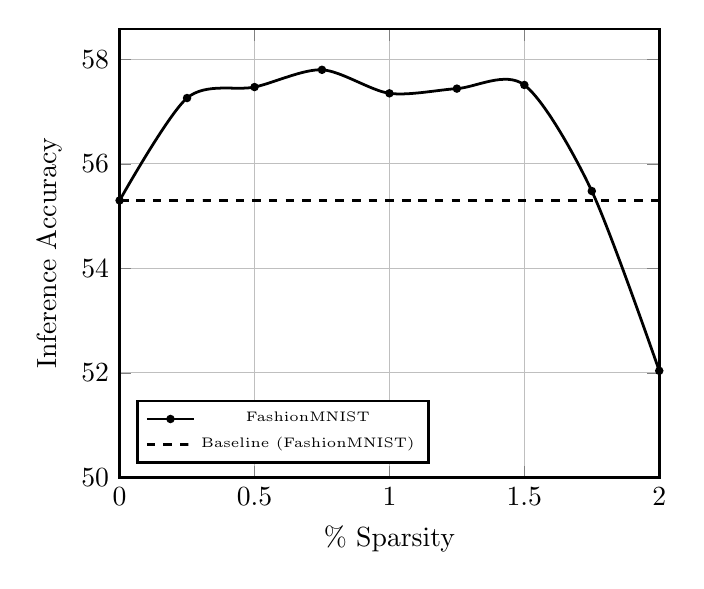
\begin{tikzpicture}
\begin{axis}[
legend style={font=\tiny},
legend pos =  south west,
line width=1.0pt,
mark size=1.0pt,
ymin=50,
xmin=0,
xmax=2,
legend entries={FashionMNIST, Baseline (FashionMNIST)},
ylabel={Inference Accuracy},
xlabel={\% Sparsity},
% extra x ticks={1,10,...,400},
% extra y ticks={0,0.5,...,10},
% extra y tick labels={},
% extra x tick labels={},
% extra x tick style={grid=major},
% extra y tick style={grid=major},
grid=major
]
\addplot[
    color=black,
    solid,
    mark=*,
    mark options={solid},
    smooth
    ]
    coordinates {
    (0,55.30)(0.25,57.26)(0.5,57.47)(0.75,57.80)(1,57.35)(1.25,57.44)(1.5,57.51)(1.75,55.48)(2,52.04)
      };
\addplot[
    color=black,
    dashed,
    smooth
    ]
    coordinates {
    (0,55.30)(0.25,55.30)(0.5,55.30)(0.75,55.30)(1,55.30)(1.25,55.30)(1.5,55.30)(1.75,55.30)(2,55.30)
      };
\end{axis}
\end{tikzpicture} &


%
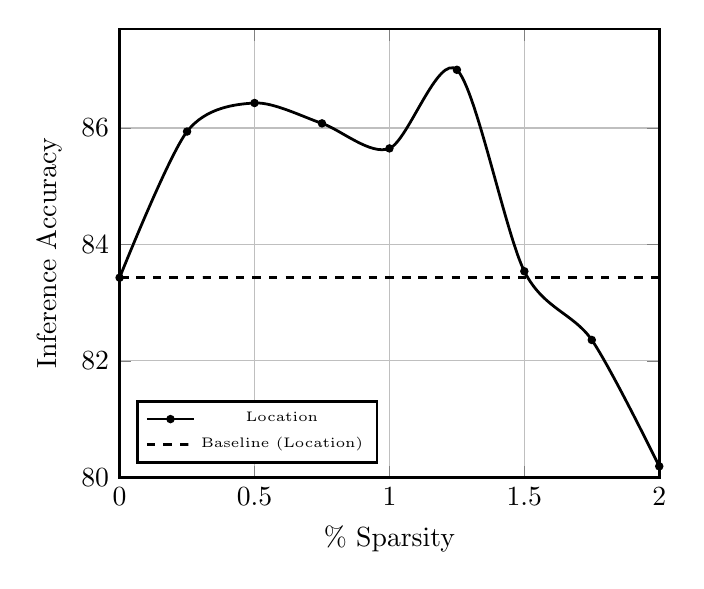
\begin{tikzpicture}
\begin{axis}[
legend style={font=\tiny},
legend pos =  south west,
line width=1.0pt,
mark size=1.0pt,
ymin=80,
xmin=0,
xmax=2,
legend entries={Location, Baseline (Location)},
ylabel={Inference Accuracy},
xlabel={\% Sparsity},
grid=major
]
\addplot[
    color=black,
    solid,
    mark=*,
    mark options={solid},
    smooth
    ]
    coordinates {
    (0,83.43)(0.25,85.94)(0.5,86.43)(0.75,86.08)(1,85.65)(1.25,87.00)(1.5,83.54)(1.75,82.36)(2,80.19)
      };
\addplot[
    color=black,
    dashed,
    smooth
    ]
    coordinates {
    (0,83.43)(0.25,83.43)(0.5,83.43)(0.75,83.43)(1,83.43)(1.25,83.43)(1.5,83.43)(1.75,83.43)(2,83.43)
      };

\end{axis}
\end{tikzpicture} &





%
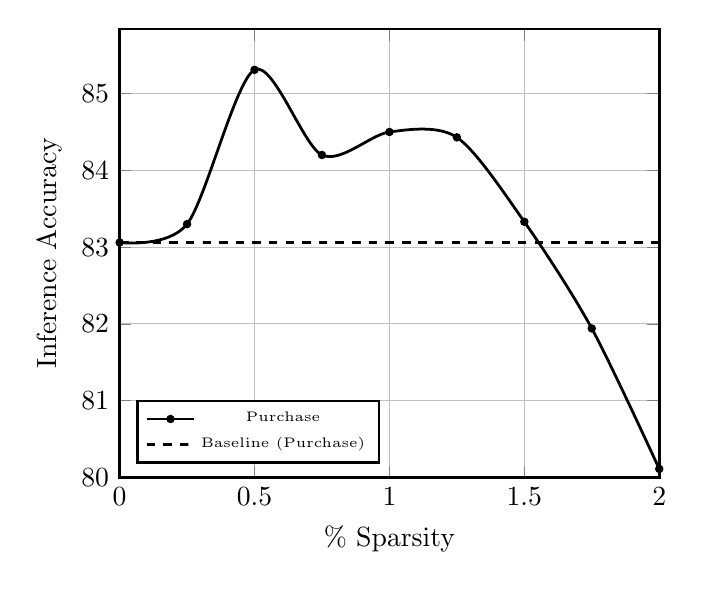
\begin{tikzpicture}
\begin{axis}[
legend style={font=\tiny},
legend pos =  south west,
line width=1.0pt,
mark size=1.0pt,
ymin=80,
xmin=0,
xmax=2,
legend entries={Purchase, Baseline (Purchase)},
ylabel={Inference Accuracy},
xlabel={\% Sparsity},
grid=major
]
\addplot[
    color=black,
    solid,
    mark=*,
    mark options={solid},
    smooth
    ]
    coordinates {
    (0,83.06)(0.25,83.30)(0.5,85.31)(0.75,84.20)(1,84.50)(1.25,84.43)(1.5,83.33)(1.75,81.94)(2,80.11)
      };
\addplot[
    color=black,
    dashed,
    smooth
    ]
    coordinates {
    (0,83.06)(0.25,83.06)(0.5,83.06)(0.75,83.06)(1,83.06)(1.25,83.06)(1.5,83.06)(1.75,83.06)(2,83.06)
      };

\end{axis}
\end{tikzpicture}


\end{tabular}
}
\caption{.}
\label{fig:loss}
\end{center}
\end{figure*}

\begin{figure*}[ht!]
\begin{center}% note that \centering uses less vspace...
\resizebox{2\columnwidth}{!}{%
\begin{tabular}{lllll}


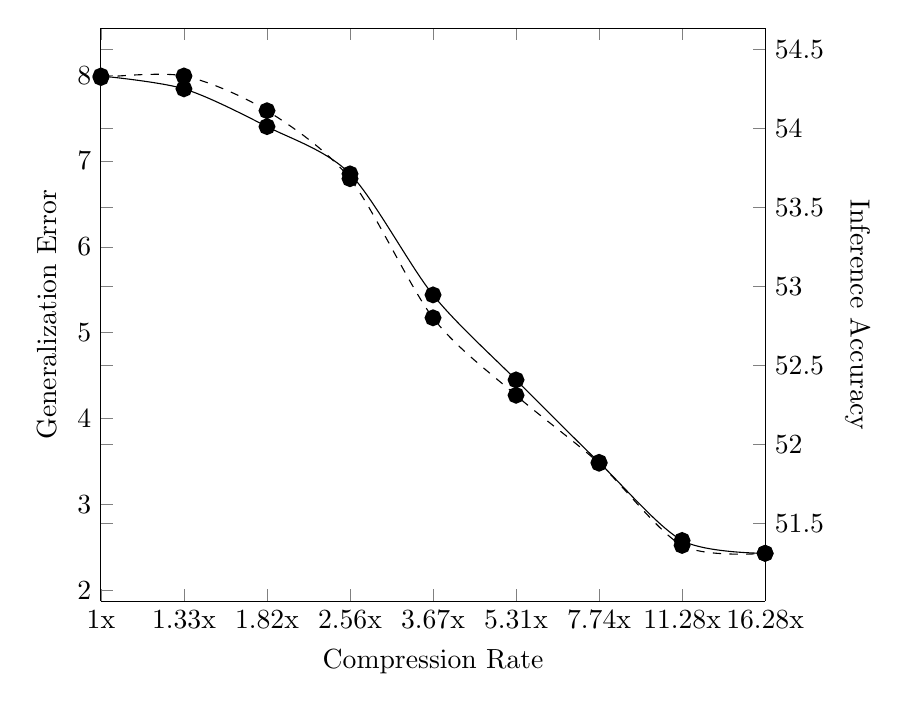
\begin{tikzpicture}
% let both axes use the same layers
\pgfplotsset{set layers}
%
\begin{axis}[
scale only axis,
line width=2.0pt,
mark size=2.0pt,
xmin=0,xmax=8,
ylabel={Generalization Error},
axis y line*=left,
xlabel={Compression Rate},
xtick={0,1,2,3,4,5,6,7,8},
xticklabels={1x, 1.33x, 1.82x, 2.56x, 3.67x, 5.31x, 7.74x, 11.28x, 16.28x}
]
\addplot[
    color=black,
    solid,
    mark=*,
    mark options={solid},
    smooth
    ]
    coordinates {
    (0,7.99)(1,7.84)(2,7.4)(3,6.85)(4,5.44)(5,4.45)(6,3.49)(7,2.58)(8,2.43)
      };
\end{axis}

\begin{axis}[
scale only axis,
line width=2.0pt,
mark size=2.0pt,
xmin=0,xmax=8,
ylabel near ticks, yticklabel pos=right,
ylabel={Inference Accuracy},
ylabel style = {rotate=180},
axis x line=none
]
\addplot[
    color=black,
    dashed,
    mark=*,
    mark options={solid},
    smooth
    ]
    coordinates {
    (0,54.32)(1,54.33)(2,54.11)(3,53.68)(4,52.80)(5,52.31)(6,51.88)(7,51.36)(8,51.31)
        };
\end{axis}
\end{tikzpicture} &

%
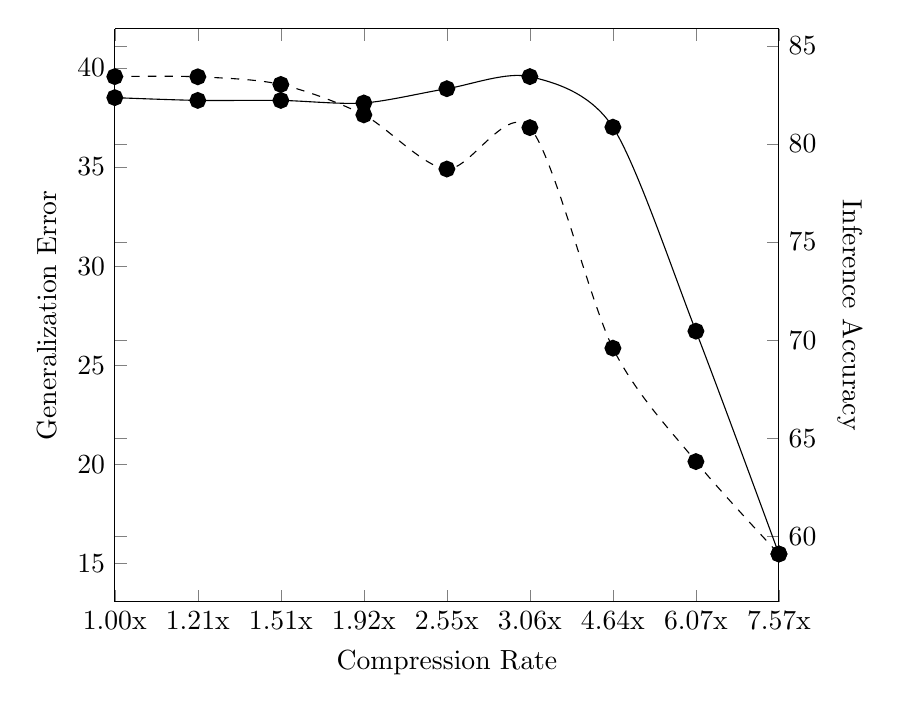
\begin{tikzpicture}
% let both axes use the same layers
\pgfplotsset{set layers}
%
\begin{axis}[
scale only axis,
line width=2.0pt,
mark size=2.0pt,
xmin=0,xmax=8,
ylabel={Generalization Error},
axis y line*=left,
xlabel={Compression Rate},
xtick={0,1,2,3,4,5,6,7,8},
xticklabels={1.00x, 1.21x, 1.51x, 1.92x, 2.55x, 3.06x, 4.64x, 6.07x, 7.57x}
]
\addplot[
    color=black,
    solid,
    mark=*,
    mark options={solid},
    smooth
    ]
    coordinates {
    (0,38.5)(1,38.36)(2,38.36)(3,38.23)(4,38.95)(5,39.56)(6,37.01)(7,26.72)(8,15.48)
      };
\end{axis}

\begin{axis}[
scale only axis,
line width=2.0pt,
mark size=2.0pt,
xmin=0,xmax=8,
ylabel near ticks, yticklabel pos=right,
ylabel={Inference Accuracy},
ylabel style = {rotate=180},
axis x line=none
]
\addplot[
    color=black,
    dashed,
    mark=*,
    mark options={solid},
    smooth
    ]
    coordinates {
    (0,83.43)(1,83.42)(2,83.03)(3,81.48)(4,78.72)(5,80.83)(6,69.59)(7,63.81)(8,59.10)
        };
\end{axis}
\end{tikzpicture} &





%
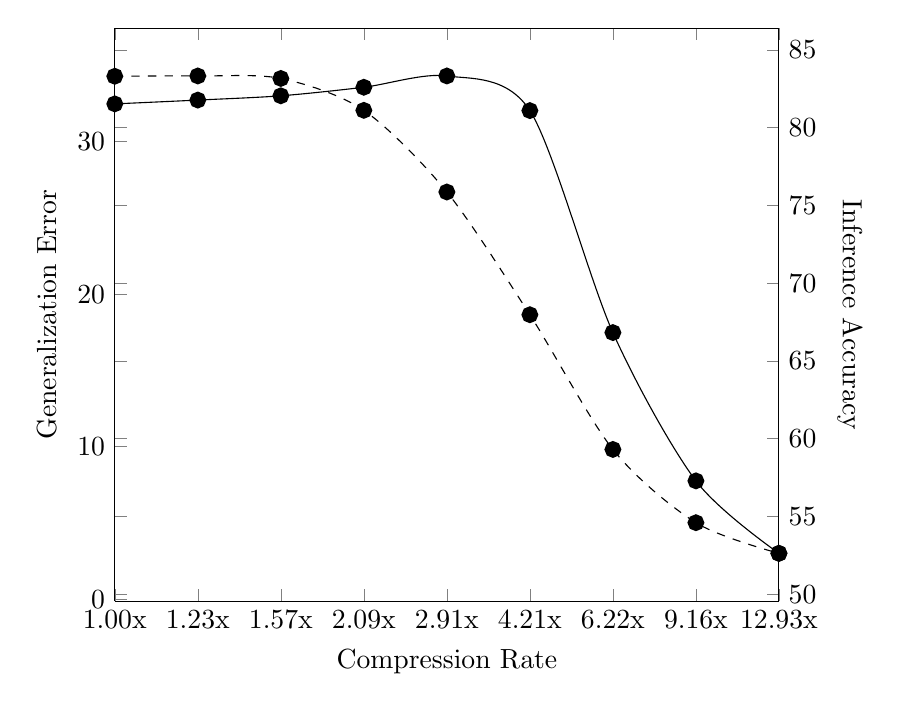
\begin{tikzpicture}
% let both axes use the same layers
\pgfplotsset{set layers}
%
\begin{axis}[
scale only axis,
line width=2.0pt,
mark size=2.0pt,
xmin=0,xmax=8,
ylabel={Generalization Error},
axis y line*=left,
xlabel={Compression Rate},
xtick={0,1,2,3,4,5,6,7,8},
xticklabels={1.00x, 1.23x, 1.57x, 2.09x, 2.91x, 4.21x, 6.22x, 9.16x, 12.93x}
]
\addplot[
    color=black,
    solid,
    mark=*,
    mark options={solid},
    smooth
    ]
    coordinates {
    (0,32.47)(1,32.72)(2,33)(3,33.56)(4,34.3)(5,32.03)(6,17.48)(7,7.76)(8,3.01)
      };
\end{axis}

\begin{axis}[
scale only axis,
line width=2.0pt,
mark size=2.0pt,
xmin=0,xmax=8,
ylabel near ticks, yticklabel pos=right,
ylabel={Inference Accuracy},
ylabel style = {rotate=180},
axis x line=none
]
\addplot[
    color=black,
    dashed,
    mark=*,
    mark options={solid},
    smooth
    ]
    coordinates {
    (0,83.30)(1,83.32)(2,83.16)(3,81.11)(4,75.86)(5,67.97)(6,59.31)(7,54.60)(8,52.63)
        };
\end{axis}
\end{tikzpicture}


\end{tabular}
}
\caption{FashionMNIST(left) Purchase100(Center) Location(Right). Dashed is Inference accuracy, solid is generalisaton error}
\label{fig:loss}
\end{center}
\end{figure*}

\begin{figure*}[ht!]
\begin{center}% note that \centering uses less vspace...
\resizebox{2\columnwidth}{!}{%
\begin{tabular}{lllll}


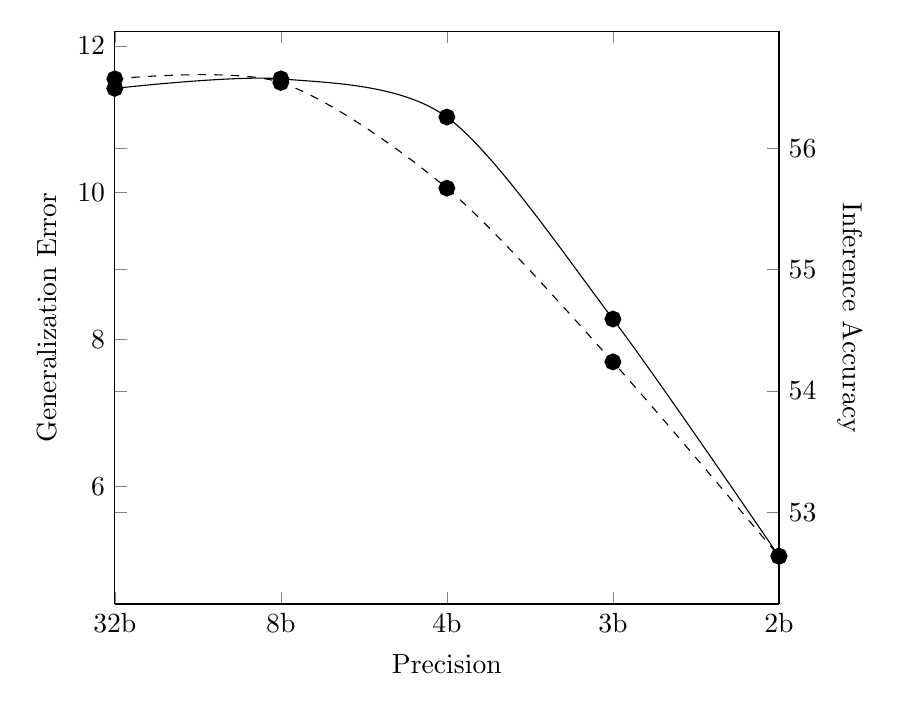
\begin{tikzpicture}
% let both axes use the same layers
\pgfplotsset{set layers}
%
\begin{axis}[
scale only axis,
line width=2.0pt,
mark size=2.0pt,
xmin=0,xmax=4,
ylabel={Generalization Error},
axis y line*=left,
xlabel={Precision},
xtick={0,1,2,3,4},
xticklabels={32b, 8b, 4b, 3b, 2b}
]
\addplot[
    color=black,
    solid,
    mark=*,
    mark options={solid},
    smooth
    ]
    coordinates {
    (0,11.42)(1,11.55)(2,11.03)(3,8.28)(4,5.05)
      };
\end{axis}

\begin{axis}[
scale only axis,
line width=2.0pt,
mark size=2.0pt,
xmin=0,xmax=4,
ylabel near ticks, yticklabel pos=right,
ylabel={Inference Accuracy},
ylabel style = {rotate=180},
axis x line=none
]
\addplot[
    color=black,
    dashed,
    mark=*,
    mark options={solid},
    smooth
    ]
    coordinates {
    (0,56.57)(1,56.54)(2,55.67)(3,54.24)(4,52.64)
        };
\end{axis}
\end{tikzpicture} &

%
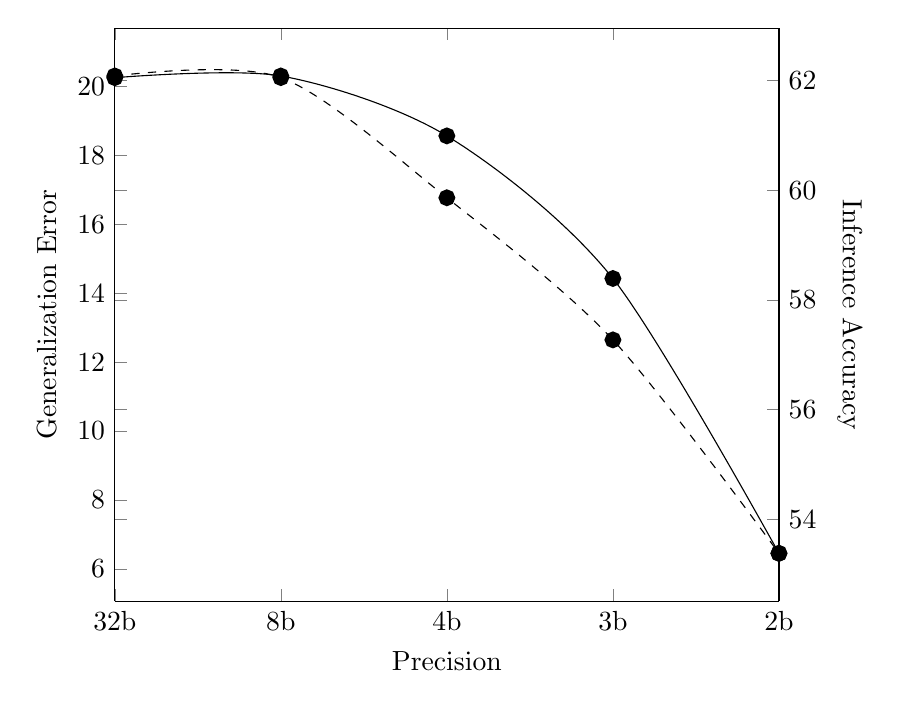
\begin{tikzpicture}
% let both axes use the same layers
\pgfplotsset{set layers}
%
\begin{axis}[
scale only axis,
line width=2.0pt,
mark size=2.0pt,
xmin=0,xmax=4,
ylabel={Generalization Error},
axis y line*=left,
xlabel={Precision},
xtick={0,1,2,3,4},
xticklabels={32b, 8b, 4b, 3b, 2b}
]
\addplot[
    color=black,
    solid,
    mark=*,
    mark options={solid},
    smooth
    ]
    coordinates {
    (0,20.26)(1,20.31)(2,18.57)(3,14.43)(4,6.45)
      };
\end{axis}

\begin{axis}[
scale only axis,
line width=2.0pt,
mark size=2.0pt,
xmin=0,xmax=4,
ylabel near ticks, yticklabel pos=right,
ylabel={Inference Accuracy},
ylabel style = {rotate=180},
axis x line=none
]
\addplot[
    color=black,
    dashed,
    mark=*,
    mark options={solid},
    smooth
    ]
    coordinates {
    (0,62.08)(1,62.05)(2,59.86)(3,57.27)(4,53.38)
        };
\end{axis}
\end{tikzpicture} &





%
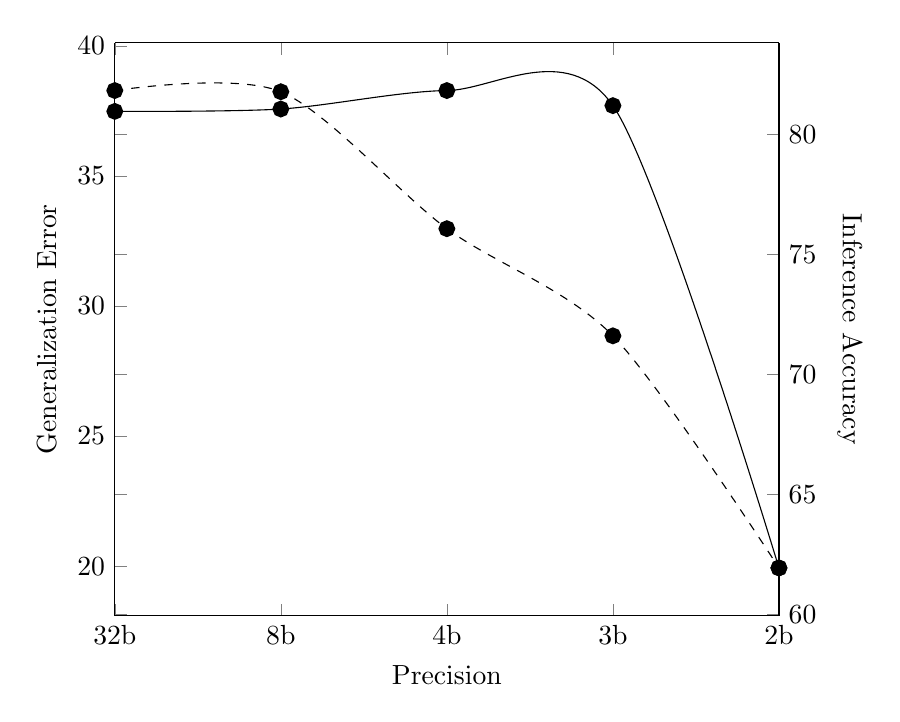
\begin{tikzpicture}
% let both axes use the same layers
\pgfplotsset{set layers}
%
\begin{axis}[
scale only axis,
line width=2.0pt,
mark size=2.0pt,
xmin=0,xmax=4,
ylabel={Generalization Error},
axis y line*=left,
xlabel={Precision},
xtick={0,1,2,3,4},
xticklabels={32b, 8b, 4b, 3b, 2b}
]
\addplot[
    color=black,
    solid,
    mark=*,
    mark options={solid},
    smooth
    ]
    coordinates {
    (0,37.48)(1,37.57)(2,38.28)(3,37.70)(4,19.93)
      };
\end{axis}

\begin{axis}[
scale only axis,
line width=2.0pt,
mark size=2.0pt,
xmin=0,xmax=4,
ylabel near ticks, yticklabel pos=right,
ylabel={Inference Accuracy},
ylabel style = {rotate=180},
axis x line=none
]
\addplot[
    color=black,
    dashed,
    mark=*,
    mark options={solid},
    smooth
    ]
    coordinates {
    (0,81.82)(1,81.77)(2,76.07)(3,71.61)(4,61.95)
        };
\end{axis}
\end{tikzpicture}


\end{tabular}
}
\caption{\underline{Pruning followed by Weight Sharing (Quantization).} While the retraining after pruning is necessary to restore the predictive accuracy, clustering the weights to reduce the precision lowers the inference accuracy (dashed line) risk while reducing the generalization error (solid line) for FashionMNIST(left), Purchase100(Center) and Location(Right) dataset.}
\label{fig:loss}
\end{center}
\end{figure*}


\noindent\textbf{Computation Efficiency.} Design of efficient off-the-shelf architectures replaces the complex matrix-vector multiplications by multiple matrix-vector multiplications with smaller dimensions.
This reduces the overall number of parameters but it has been shown empirically\footnote{https://github.com/albanie/convnet-burden} that this does not necessarily reduce the number of multiply accumulate operations or FLOPS~\cite{article}.
In case of parameter pruning, achieving efficiency requires additional hardware optimization. Particularly, instead of actually computing the the multiplications with "0"pruned values, the hardware optimization enable the user to skip the computation and replace the output by a "0" directly.
For quantized models with binarized parameters and activations the MAC operations can be replaced by binary operations such as XNOR and the maxpool operations can be replaced by OR operation, while the activations can be replaced by checking the parity bit (denotes the sign) operation and hence reducing the FLOPS drastically[XONN].
This results in high computational efficiency and hence, faster inference.


\noindent\textbf{Energy Efficiency.} Energy efficiency has been shown to not vary much in case of reduction with number of parameters and data type, number of memory accesses play vital role[CVPR 2017 yang et al][].
Specifically, for the case of off-the-shelf architectures the while the computation efficiency has been shown to improve, the energy efficiency has been shown to be close to large scale state of the art models like AlexNet[suqeezenet][].
Alternatively, for the case of model compression, energy efficiency can be achieved by additionally providing hardware optimization and shows small improvement in the energy consumption[].
For quantization, however, the energy efficiency has been shown to be high [][] where the memory access can be drastically reduced by increasing the throughput of data fetched from the memory.
Specifically, lowering the precision from 32 bit floating point to binary results in lowering the memory accesses and 32x improvement in energy consumption[][][].
While some improvement is seen natively for quantized models (from replacing MACs with XNOR), higher benefits can be achieved via additional hardware optimization[].
The benchmarking of energy consumption for different optimization and architectures is well explored in the literature and out of scope of this work. We refer the authors to [][][] for more details.

In summary, compared to different optimization techniques for NNs, the quantized architectures show significant benefit for different efficiency requirements over the other alternatives.




\subsection{Evaluating Privacy Leakage}

In this section, we evaluate the information leakage through membership inference attacks for the three baseline algorithms considered.
This is the main contribution of our work where we evaluate the privacy leakage for different optimization and design algorithms for NNs.

\subsubsection{Model Compression}

We evaluate the privacy leakage on compressing a model by pruning the connections in the model.
Here, pruning is achieved by replacing some of the parameters with "0" value.
As described in the original paper~\cite{}, pruning is followed by retraining the model to restore the model's original accuracy with the pruned connections.

We evaluate and validate the impact on membership privacy on compressing the model trained on three datasets: FashionMNIST, Location and Purchase100.
On pruning the model, the model's test accuracy decreases but also lowers the membership inference accuracy (Figure~\ref{fig:prune}).
This is expected as the parameters are responsible for memorizing the training data information and pruning the parameters lowers the adversary's attack success~\cite{rezawhite}.

However, interestingly, on retraining the pruned model, we observe that the membership inference accuracy is much higher than the original unpruned baseline model (Figure~\ref{fig:retrain}).
This indicates that model compression in turn increases the overall privacy leakage.
This can be attributed to the lower number of parameters forced to learn the same amount of information stored previously in the unpruned model with larger number of parameters.
In other words, the same amount of information is now captured by less number of parameters resulting in higher memorization of information per parameter.
To analyze the information stored per parameter, we first compute the model capacity as the mutual information of a trained network between the true label $Y$ and the predicted label $Y_{\theta}$ for a random input $X$ as derived in~\cite{45932,cap}.
Here, model's information $I(Y;Y_{\theta}|X) = $
\begin{equation}
\footnotesize
N_{train}\left(1 - (r_{train}log_2(\frac{1}{r_{train}}) + (1-r_{train})log_2(\frac{1}{1-r_{train}}))\right)
\end{equation}
where $r_{train}$ is the classification train accuracy for all the $N_{train}$ samples in the training data.
For $r_{train} = 1$, the model completely memorizes all random samples as the information stored equals the number of samples $N_{train}$, while for $r_{train}=0.5$, the training accuracy 0.
We divide the above equation by the model's total number of parameters $N_{param}$ to get the per parameter information stored as
\begin{equation}
I_p(Y;Y_{\theta}|X) = \frac{I(Y;Y_{\theta}|X)}{N_{param}}
\end{equation}
As the model is compressed (pruned), the number of parameters $N_{param}$ decreases which results in increase in $I_p(Y;Y_{\theta}|X)$. However, on aggressive pruning, the train accuracy $r_{train}$ also decreases resulting in a decrease in the information per parameter, which is empirically indicated by a decrease in membership inference accuracy at the end in Figure~\ref{fig:retrain}.


\textbf{Mitigating the Privacy Risks in Pruned Models.} We describe on potential approach to mitigate the privacy risk of the compressed models without requiring to modify the model's training.
The post-hoc apporach utilizes the weight sharing for the compressed model. This is however, accompanied by a decrease in the model's prediction accuracy indicating a privacy-utility trade-off.
As seen in Figure~\ref{fig:wtsharing}, reducing the precision from 32 bits to 2 bits results in a decrease in inference accuracy from 56.57\% to 52.64\% for FashionMNIST, 62.08\% to 53.38\% for Location and 81.82\% to 61.95\% for Purchase100 dataset.
This decrease in inference attack accuracy is closely followed by a decrease in generalization error which is indicative of decrease in prediction accuracy of the model.
We evaluate the effectiveness of pruning followed by quantization which has been shown to have significant impact on reducing the model complexity through compression more significantly than either pruning or quantization alone.
For the experiments, we use the compressed model indicating highest privacy leakage to evaluate the effectiveness of weight sharing on the worst case condition.
This pipelined approach of pruning followed by retraining followed by weight sharing, not only maintains the algorithm's objective for efficiency but is used as a post-hoc approach to reduces the overall inference risk~\cite{DBLP:journals/corr/HanMD15,DBLP:journals/corr/HanPNMTECTD16}.






\subsubsection{Off-the-Shelf Efficient Architectures}


\begin{table}[!htb]
\begin{center}
\renewcommand\arraystretch{1.5}
\fontsize{6.7pt}{6.7pt}\selectfont
\begin{tabular}{|c|c|c|c|c|}
\hline
\textbf{Architecture} & \textbf{Memory} & \textbf{Train}  & \textbf{Test}  & \textbf{Inference}   \\
 & \textbf{Footprint} & \textbf{Accuracy} & \textbf{Accuracy} & \textbf{Accuracy}  \\
\hline
SqueezeNet & 5 MB & 88.21\% & 81.92\% & \cellcolor{green!25}53.07\% \\
MobileNetV2 & 14 MB & 97.50\% & 87.24\% & \cellcolor{green!25}55.57\% \\
\hline
AlexNet & 240 MB & 97.86\% & 80.34\% & \cellcolor{red!25}60.40\% \\
VGG11 & 507 MB & 99.13\% & 86.43\% & \cellcolor{red!25}58.04\% \\
VGG16 & 528 MB & 99.58\% & 88.95\% & \cellcolor{red!25}58.70\%  \\
VGG19 & 549 MB & 99.09\% & 88.18\% & \cellcolor{red!25}57.85\% \\
\hline
\end{tabular}
\end{center}
\caption{Model complexity influences the membership inference leakage. Model specifically designed for efficiency leak less information.}
\label{stdarch}
\end{table}

In this section, we evaluate two popular state of the art architectures, SqueezeNet and MobileNet, trained on CIFAR10 dataset used for low powered systems.
As seen in Table~\ref{stdarch}, the SqueezeNet and MobileNet models shows lower inference accuracy of 53.07\% and 55.57\% compared to larger models which have higher privacy leakage.

\begin{figure}[hb!]
\resizebox{0.8\columnwidth}{!}{%
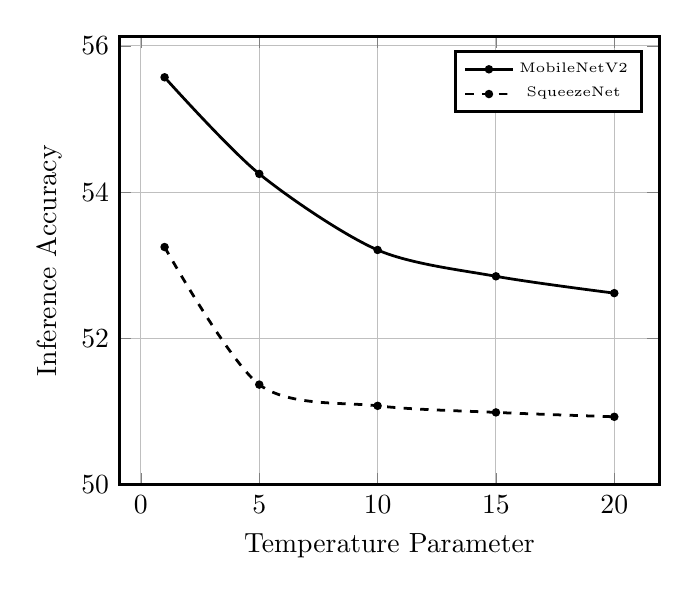
\begin{tikzpicture}
\begin{axis}[
legend style={font=\tiny},
legend pos =  north east,
line width=1.0pt,
mark size=1.0pt,
ymin=50,
legend entries={MobileNetV2, SqueezeNet},
ylabel={Inference Accuracy},
xlabel={Temperature Parameter},
% extra x ticks={1,10,...,400},
% extra y ticks={0,0.5,...,10},
% extra y tick labels={},
% extra x tick labels={},
% extra x tick style={grid=major},
% extra y tick style={grid=major},
grid=major
]
\addplot[
    color=black,
    solid,
    mark=*,
    mark options={solid},
    smooth
    ]
    coordinates {
    (1,55.57)(5,54.25)(10,53.21)(15,52.85)(20,52.62)
      };
\addplot[
      color=black,
      dashed,
      mark=*,
      mark options={solid},
      smooth
    ]
    coordinates {
    (1,53.25)(5,51.37)(10,51.08)(15,50.99)(20,50.93)
      };
\end{axis}
\end{tikzpicture}
}
\caption{The privacy leakage of models designed for efficiency (SqueezeNet and MobileNet) can be reduced by increasing the softmax temperature. }
\end{figure}


Further, the inference accuracy of SqueezeNet and MobileNet can be further reduced close to random guess by increasing the temperature parameter of the softmax function applied to the output.
Increasing the temperature parameter reduces the granularity of the model's output and is given by $F_i(x) = \frac{e^{\frac{z_i(x)}{T}}}{\sum_{j}e^{\frac{z_j(x)}{T}}}$ where $z(x)$ computes output of the model before the softmax layer.
For the case of SqueezeNet, we are able to reduce the inference accuracy to 50.93\% from 53.07\% while for MobileNet we can reduce the inference accuracy to 52.62\% from 55.57\% as seen in Figure~\ref{softmax}.
This reduction in inference accuracy is without any cost of the prediction test accuracy of the model.




\subsubsection{Quantization}

In this section, we evaluate the technique of reducing the precision of both model's parameters and intermediate activations.
Further, we consider the extreme case of binarizing the parameters and activations allowing to evaluate on the most optimized case.
We evaluate on FashionMNIST dataset for two architectures with convolutional and fully connected layers.

\begin{table}[!htb]
\begin{center}
\renewcommand\arraystretch{1.5}
\fontsize{6.7pt}{6.7pt}\selectfont
\begin{tabular}{|c|c|c|c|c|}
\hline
\multicolumn{5}{|c|}{\textbf{FashionMNIST}}\\
\hline
\textbf{Architecture} & \textbf{Memory} & \textbf{Train}  & \textbf{Test}  & \textbf{Inference}  \\
 & \textbf{Accuracy} &  \textbf{Footprint} & \textbf{Accuracy} & \textbf{Accuracy}  \\
\hline
\multicolumn{5}{|c|}{Architecture 1}\\
Full & 38.39 MB & 100\% & 92.35\% & \cellcolor{red!25}57.46\%\\
BinaryNet & 1.62 MB & 88.68\% & 86.9\% & \cellcolor{green!25}55.45\%\\
XNOR-Net & 1.62 MB & 87.19\% & 85.68\% & \cellcolor{green!25}51.05\%\\ %1,626,824 parameters
\hline
\multicolumn{5}{|c|}{Architecture 2}\\
Full & 29.83 MB & 99.34\% & 89.88\% & \cellcolor{red!25}54.86\% \\
BinaryNet & 0.93 MB & 97.61\% & 89.60\% & \cellcolor{green!25}54.30\%\\
XNOR-Net & 0.93 MB & 92.67\% & 86.68\% & \cellcolor{green!25}51.74\%\\ %937,000parameters
\hline
\end{tabular}
\end{center}
\caption{Reducing the model precision lowers the inference attack accuracy but at the cost of test accuracy.}
\label{fmnist_quantize}
\end{table}

In both the architectures, we see that computation on  binarized parameters and activations reduces the inference risk by a small value.
However, on replacing the MAC operations with XNOR operations, we observe that the inference risk decreases close to random guess, however, at the cost of prediction test accuracy.

In summary, we observe that quantization, specifically binarization of parameters and activation along with XNOR computation, provides strong resistance against inference attacks compared to model compression and off-the-shelf architectures.

\subsection{Summary of Comparison}

We summarize the properties satisfied by each of the technique in terms of privacy, computation, memory and energy efficiency in Table~\ref{tbl:comparison}.
Here, we mark the attributes which are satisfied with $\cmark$, requires additional hardware optimization as $\smark$ and does not satisfy the property with a $\xmark$.

\begin{table}[!htb]
\begin{center}
\renewcommand\arraystretch{1.5}
\fontsize{6.7pt}{6.7pt}\selectfont
\begin{tabular}{|l||l|l|l|}
\hline
Requirements & Compression & Quantization & Off-the-shelf  \\
\hline
Computation Efficiency & $\smark$  & $\cmark$   & $\xmark$ \\
\hline
Memory Efficiency &  $\smark$ & $\cmark$   & $\cmark$ \\
\hline
Energy Efficiency &  $\smark$   & $\cmark$   & $\xmark$ \\
\hline
Privacy &  $\xmark$   & $\cmark$   & $\smark$ \\
\hline
\end{tabular}
\end{center}
\caption{Comparison of different optimizations for NNs. $\smark$: additional hardware optimization; $\xmark$: requirement not satisfied; $\cmark$: requirement satisfied.}
\label{tbl:comparison}
\end{table}

For our requirement, quantization of NNs is an attractive design choice which not only satisfies the computation, memory and energy efficiency but also provides high resistance against inference attacks.
Specifically, in this work we only consider the aggressive quantization of binarizing the parameters and activations to \{-1,+1\} values while additionally replacing the MAC operations with cheap and efficient binary arithmetic (XNOR operations).
Hence, we choose this particular design for NNs to provide a good three dimensional trade-off between privacy-efficiency-accuracy.





\section{Experimental setting}
\label{setting}

We carried out an extensive evaluation of \method. %the three state of the art design techniques for efficient model computation.
%: a) Model Compression via pruning redundant parameters and nodes, b) Quantization to lower the precision of model parameters and activations, and c) Efficient off-the-shelf architectures.
%
%We show that ... In addition, we show that ...
We first describe the datasets and architectures used in this analysis (Section~\ref{datasets}) before to present the considered comparative baselines (Section~\ref{baselines}) and metrics (Section~\ref{metrics}). %Finally, we analyse efficiency Section~\ref{eval-efficiency} and privacy leakage Section~\ref{eval-leakage}.


\subsection{Datasets and Architectures}
\label{datasets}

For evaluating and comparing different efficiency algorithms, we use two standard benchmarking datasets: FashionMNIST and CIFAR10.
We train the model for 75 epochs for FashionMNIST and 100-150 epochs for CIFAR10.
%For FashionMNIST dataset we train the model for 75 epochs and for CIFAR10, we train the models for 100-150 epochs.
%These provide us with the necessary direction to choose the optimal efficiency algorithm which satisfies all the efficiency and privacy requirement as describes in Section~\ref{motivate}.

\noindent\textbf{FashionMNIST.} This dataset consists of 60,000 training examples and a test set of 10,000 examples.
Each data record is a 28$\times$28 grayscale image which is mapped to one of 10 classes consisting of fashion products such as coat, sneaker, shirt, shoes.
For this dataset, we use a modified LeNet architecture with two convolution layers followed by maxpool and dense layers: [Conv 32 (3,3), Conv 64 (3,3), Maxpool (2,2), Dense 128, Dense 10] (Architecture 1). Additionally, we use a fully connected model [512,512,512] (Architecture 2).

\noindent\textbf{CIFAR10}. This dataset is a major image classification benchmarking dataset where the data records are composed of 32$\times$32 RGB images where each record is mapped to one of 10 classes of common objects such as airplane, bird, cat, dog.
For this dataset, we use standard state of the art architectures: Network in Network (NiN), AlexNet and VGGNet.


\subsection{Comparative Baselines}
\label{baselines}

\subsubsection{NN models for embedded systems}

%In order to execute trained NN models on low powered edge devices, optimizations are required for the design of the NN architectures.
Model designers use three state of the art approaches for designing efficient NN models for embedded systems: (a) Model Compression via Pruning, (b) quantization of model parameters and activations and (c) designing standard architectures (off the shelf efficient architectures).
%In this work, we consider these three approaches as baselines for comparison and evaluation to select the choice of optimization for \method.

\begin{itemize}[leftmargin=*]

\item {\em Model Compression (Pruning).}
NNs are overparameterized, i.e, have a large number of redundant weights.
Pruning the network refers to removing these redundant weights (setting them as zero) without a degradation of model accuracy.
The pruning operation results in a model with sparse parameters for which the hardware can be designed to skip the multiplication and memory storage, improving the efficiency.
Sparse weights can be stored in a compressed format in the hardware using the compressed sparse row or column format which reduces the overall memory bandwidth~\cite{DBLP:journals/corr/HanMD15,10.1109/ISCA.2016.30,Han:2015:LBW:2969239.2969366}.
Aggressive pruning, while compressing the model significantly, requires to be re-trained to restore the model's original accuracy.
For a sensitivity threshold $T$, the parameters close to zero are replaced by zero: % which is given as:
\[
\footnotesize
    f(W)=
\begin{cases}
    0, & \text{if } -T \leq w \leq T\\
    w,  & \text{otherwise}
\end{cases}
\]

\item {\em Off-the-Shelf Efficient Architectures.}
NNs can be redesigned by changing the hyperparameters (i.e., filter size in convolution, number of layers and their types) to reduce the number of parameters and hence, the memory footprint.
One approach is to replace larger convolution filters with multiple smaller filters with less number of parameters but covering the same receptive fields.
For instance, one 5x5 filter can be replaced by two 3x3 filters.
Alternatively, 1x1 convolutional layers reduce the number of channels in output feature map, lowering the computation and number of parameters.
For instance, for an input activation of dimension 1x1x64, 32 1x1 convolutional filters downsamples the activation maps to get an output of 32 channels.
Such optimizations enable to design compact network architecture with layers having lower parameters compared to the original model, extensively adopted in MobileNet~\cite{conf/cvpr/SandlerHZZC18} and SqueezeNet~\cite{DBLP:journals/corr/IandolaMAHDK16}.


\item {\em Quantization.}
Quantization reduces the precision of the model's parameters and the intermediate activations during execution.
Quantization maps parameters and activations to a fixed set of quantization levels~\cite{Hubara:2017:QNN:3122009.3242044}.
The number of quantized levels determines the precision of the operands ($log_2(\#levels)$).
Reducing the precision of the (a) parameters lowers the storage cost of the model in memory, (b) activations lowers the computation overhead by replacing MACs with binary arithmetic and (c) reduces the energy consumption by lowering the memory accesses and increasing throughput.
Aggressively quantizing the parameters and activations to binary and ternary precision significantly improves the overall efficiency, however, at the cost of accuracy~\cite{rastegari2016xnornet}.
For instance, Binarized NNs quantize the operands to \{-1,+1\} values~\cite{NIPS2016_6573} while ternary NNs have values \{-w, 0, w\} where $w$ can be fixed or learnt during training~\cite{Li2016TernaryWN}. These are examples of uniform quantization.
Alternatively, weight sharing maps several parameters to a single value reducing the number of unique parameters~\cite{DBLP:journals/corr/HanMD15}.
%This mapping is done using K-Means clustering or a hashing function and the corresponding shared values are read from a "codebook" which maps different parameters to its shared value.
This mapping is done using K-Means clustering or a hashing function where a "codebook" maps different parameters to the corresponding shared values.

\end{itemize}


\subsubsection{Privacy defences}


%In this work,
We consider two state of the art baselines: Adversarial Regularization and Differential Privacy.
These defences have mainly focussed on improving the model's generalization and reduce overfitting which has been considered as the main cause for leakage through membership inference attacks.

\begin{itemize}[leftmargin=*]
\item {\em Adversarial Regularization (AdvReg)~\cite{DBLP:conf/ccs/NasrSH18}.} Here, the problem of defending against membership inference attack is modelled as a minimax game between two NNs: classifier network and attacker network.
The two networks are trained alternatively with conflicting objectives: first, the attacker network is trained to distinguish between the training data members and non-members followed by training the classifier network to minimize the loss as well as fool the attacker network.
Formally, the target classifier outputs a single probability $I(F(x),y) \in [0,1]$ which indicates the likelihood of $x$ being part of the training data.
The classifier minimizes the loss along with the output of the attacker classifier balanced with a privacy risk hyperparameter $\lambda$ : $min_{\theta} l(F(x),y) + \lambda log(I(F(x),y))$.

\item {\em Differential Privacy (DP)~\cite{Abadi:2016:DLD:2976749.2978318}.} In this work, we specifically consider DP-SGD which adds carefully crafted noise to the gradients during backpropagation in SGD algorithm.
The noise is sampled from a Laplacian or Gaussian distribution proportional to the model's sensitivity which is then added to the gradients during backpropagation.
This provides provable bound on the information leaked about an individual data record in the dataset and ensures that the presence or absence of a data record does not change the model's output, hence defending against membership inference attacks.
\end{itemize}

\subsection{Metrics}
\label{metrics}

\noindent\textbf{Efficiency.} We evaluate efficiency on Memory efficiency, Computation efficiency and Energy efficiency. Memory efficiency is compared based on the reduction in the memory footprint of the model computed from the parameters stored in the memory. Computation efficiency is compared based on the reduction in the MAC operations which influences the execution time. Finally, the energy consumption is compared based on memory accesses from reading inputs and writing results to the memory. Since, significant literature has compared the efficiency empirically~\cite{8114708}, we provide a qualitative comparison for the baseline algorithms.

\noindent\textbf{Privacy.} We use the inference attack accuracy to estimate the success of membership inference attack.
An accuracy above random guess $50\%$ indicates a training data leakage through membership inference attack.
This indicates that the adversary is able to identify the membership details of a data record with an accuracy higher than random guess.
The success of inference attack accuracy is strongly correlated with the model's extent of overfitting empirically measured as the difference between the train and test accuracy (i.e., generalization error). Higher generalization error (i.e., overfitting) results in higher distinguishability between the test and train resulting in higher membership inference accuracy~\cite{shokri2017membership}.
Additionally, the accuracy of the model is computed using the model's performance on unseen test data.

%\section{\method: Design Motivation}\label{motivate}

In this section, we describe the requirements to be satisfied while designing NNs for embedded systems within the \method\hspace{0.02in} methodology.
We motivate the NN design by comparing different efficiency optimization algorithms based on the privacy and efficiency requirements of embedded devices.
In this work, we specifically select the three state of the art design techniques for efficient model computation:\virat{didnt u mention this above? if yes, just refer to them don't rewrite}
\begin{itemize}
\item Model Compression via pruning redundant parameters and nodes
\item Quantization to lower the precision of model parameters and activations
\item Efficient off-the-shelf architectures
\end{itemize}

\virat{I don't understand the flow of this section: You state 3 requirements, but why only one is detailed? Why 3.4 is evaluation? I think you should state the overall design requirements at first, then explain each requirement in detail (why only 'efficiency' is detailed?)}

\virat{I think u need to move 3.4 up that shows the leakage, then discuss the requirements, then introduce gecko and show how it addresses the shortcomings you found in 3.4 and also the other requirements u discuss}

\subsection{Overall Design Requirements}

In designing our training methodology, \method, we aim to satisfy the following main requirements in the purview of embedded systems:

\begin{itemize}[leftmargin=*]

\item {\em Privacy-}
The model should preserve the privacy of an individual's data record in the training set of the model against inference attacks.

\item {\em Efficiency-}
The private model should demonstrate high energy, memory and computation efficiency.

\item {\em Accuracy-}
The drop in accuracy of the private model should be minimum as compared to the non-private and non-efficient model accuracy.
\end{itemize}

To this end, we present \method --- a technique to construct NNs that are optimized for efficiency and accuracy while ensuring privacy of the input data.
With \method, we present a novel approach of building NNs with efficiency as a key property.
We argue that fixing a NN architecture and then modifying the training algorithm to ensure privacy (e.g. adversarial regularization[] and differential privacy[]) does not provide optimal balance between efficiency and accuracy.
On the contrary, our approach advocates building NN architecture considering the strengths and drawbacks of the underlying algorithms to design efficient NNs.
We assert that this is a practical solution as deep learning algorithms are flexible with respect to their architectures, i.e., different NNs can be trained to achieve the same accuracy for a given dataset.


\subsection{Efficiency Requirements}

In designing \method, we make several design choices with the goal of achieving efficiency over existing solutions.
The most important among them is the selection of the underlying algorithm to design NNs with high efficiency.
Several state of the algorithms are currently adopted such as, however, these algorithm do not provide the same efficiency guarantees.
These differences make it difficult to decide which primitive is the best fit for designing a privacy-preserving system for a particular application.
Therefore, we first outline the desirable properties specifically for private NN inference:

\begin{itemize}[leftmargin=*]
\item {\em Energy Efficiency-} Energy consumption is a vital constraint for low powered embedded or IoT devices which operate for long duration while maximising their battery lifetime.
While executing NNs, every MAC requires memory access for reading weights, inputs and intermediate output from previous layer and one write to store the computed outputl which is significantly higher than actually performing the MAC operation in the CPU[].
Energy efficiency is achieved by reducing the memory access by (a) optimizing hardware to exploit sparsity in MACs and (b) reducing the precision to increase the throughput of data.

\item {\em Computation Efficiency-} The total multiply accumulate (MAC) operations between the parameter matrix and input activation function quantifies the requirement of computation efficiency.
The processing rate of MAC operations is constrained by the CPU on embedded device which is reduced by reducing the total number of parameters.
Additionally, replacing MACs with cheaper binary arithmetic significantly lowers the computational overhead.

\item {\em Memory Efficiency-} The total size of the model measured in terms of the memory storage for model parameters and additional runtime storage for intermediate outputs should be within the memory constraints of the embedded device.
This is achieved in two ways: (a) reducing the precision of the parameters and intermediate outputs and (b) pruning the parameters by increasing sparsity.
\end{itemize}

\subsection{Optimization for Efficiency}

\red{Here, in the view of the above efficiency requirements, we compare the three baseline algorithms.
We then select an efficient design scheme for NNs that satisfies all our requirements.}
\virat{why is the choice of design scheme in motivation?}

\noindent\textbf{Memory Efficiency.} Off the shelf models are designed to specifically reduce the memory footprint.
For instance, the memory footprint of Squeezenet and MobileNet is 5MB and 14Mb compared to 250Mb of Alexnet and >500Mb of VGG architectures.
Additionally, lowering the model precision from 64 or 32 bit floating point to binary precision results in a direct reduction of 64x or 32x in the overall memory footprint of the model.
However, in case of model compression the model parameters which are pruned are simply replaced by a value of "0".
Hence, storing even the "0" parameter takes up memory and does not necessarily decrease the overall memory footprint unless the hardware is optimized to skip the storage of all the zero values in the memory.
This requires additional logic to check for zero valued parameters in a dictionary.

\begin{figure*}[ht!]
\begin{center}% note that \centering uses less vspace...
\resizebox{2\columnwidth}{!}{%
\begin{tabular}{lllll}


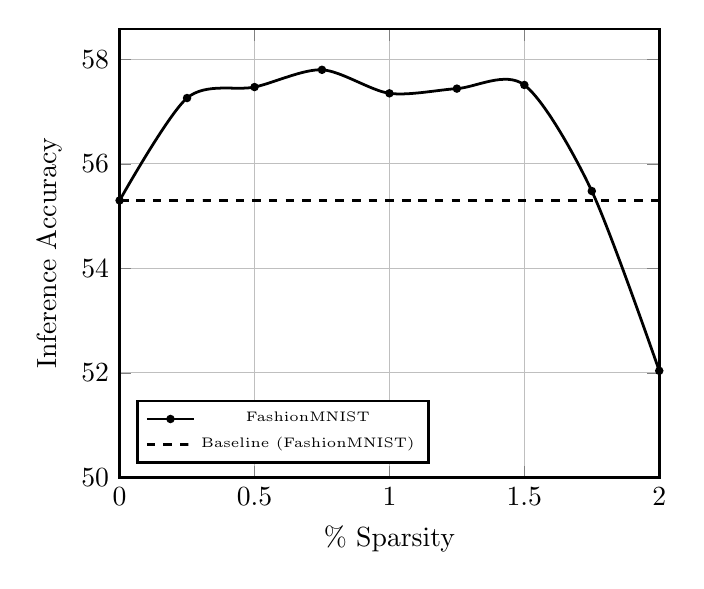
\begin{tikzpicture}
\begin{axis}[
legend style={font=\tiny},
legend pos =  south west,
line width=1.0pt,
mark size=1.0pt,
ymin=50,
xmin=0,
xmax=2,
legend entries={FashionMNIST, Baseline (FashionMNIST)},
ylabel={Inference Accuracy},
xlabel={\% Sparsity},
% extra x ticks={1,10,...,400},
% extra y ticks={0,0.5,...,10},
% extra y tick labels={},
% extra x tick labels={},
% extra x tick style={grid=major},
% extra y tick style={grid=major},
grid=major
]
\addplot[
    color=black,
    solid,
    mark=*,
    mark options={solid},
    smooth
    ]
    coordinates {
    (0,55.30)(0.25,57.26)(0.5,57.47)(0.75,57.80)(1,57.35)(1.25,57.44)(1.5,57.51)(1.75,55.48)(2,52.04)
      };
\addplot[
    color=black,
    dashed,
    smooth
    ]
    coordinates {
    (0,55.30)(0.25,55.30)(0.5,55.30)(0.75,55.30)(1,55.30)(1.25,55.30)(1.5,55.30)(1.75,55.30)(2,55.30)
      };
\end{axis}
\end{tikzpicture} &


%
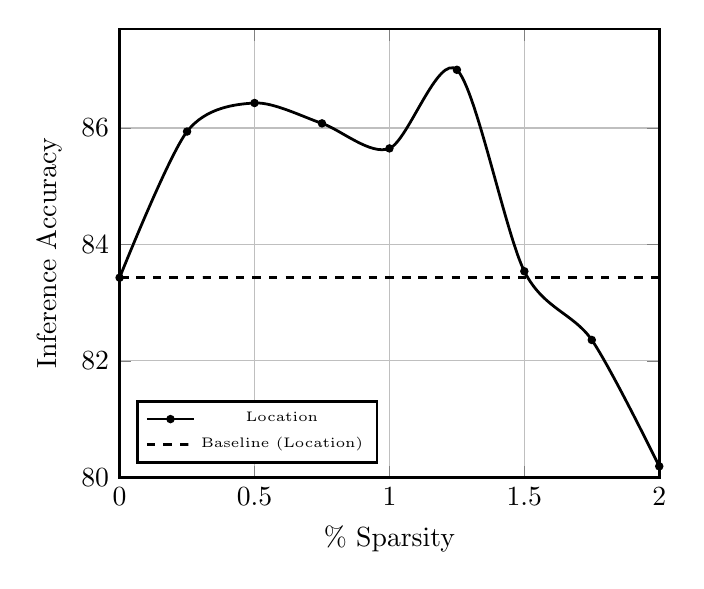
\begin{tikzpicture}
\begin{axis}[
legend style={font=\tiny},
legend pos =  south west,
line width=1.0pt,
mark size=1.0pt,
ymin=80,
xmin=0,
xmax=2,
legend entries={Location, Baseline (Location)},
ylabel={Inference Accuracy},
xlabel={\% Sparsity},
grid=major
]
\addplot[
    color=black,
    solid,
    mark=*,
    mark options={solid},
    smooth
    ]
    coordinates {
    (0,83.43)(0.25,85.94)(0.5,86.43)(0.75,86.08)(1,85.65)(1.25,87.00)(1.5,83.54)(1.75,82.36)(2,80.19)
      };
\addplot[
    color=black,
    dashed,
    smooth
    ]
    coordinates {
    (0,83.43)(0.25,83.43)(0.5,83.43)(0.75,83.43)(1,83.43)(1.25,83.43)(1.5,83.43)(1.75,83.43)(2,83.43)
      };

\end{axis}
\end{tikzpicture} &





%
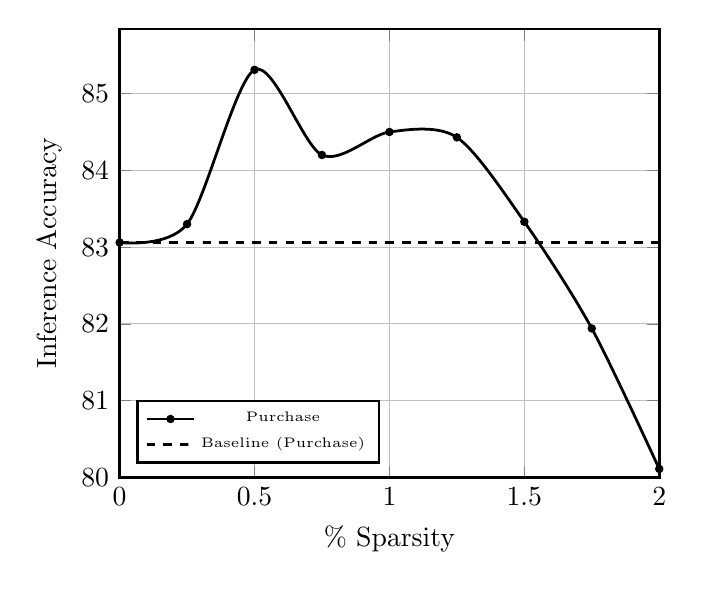
\begin{tikzpicture}
\begin{axis}[
legend style={font=\tiny},
legend pos =  south west,
line width=1.0pt,
mark size=1.0pt,
ymin=80,
xmin=0,
xmax=2,
legend entries={Purchase, Baseline (Purchase)},
ylabel={Inference Accuracy},
xlabel={\% Sparsity},
grid=major
]
\addplot[
    color=black,
    solid,
    mark=*,
    mark options={solid},
    smooth
    ]
    coordinates {
    (0,83.06)(0.25,83.30)(0.5,85.31)(0.75,84.20)(1,84.50)(1.25,84.43)(1.5,83.33)(1.75,81.94)(2,80.11)
      };
\addplot[
    color=black,
    dashed,
    smooth
    ]
    coordinates {
    (0,83.06)(0.25,83.06)(0.5,83.06)(0.75,83.06)(1,83.06)(1.25,83.06)(1.5,83.06)(1.75,83.06)(2,83.06)
      };

\end{axis}
\end{tikzpicture}


\end{tabular}
}
\caption{.}
\label{fig:loss}
\end{center}
\end{figure*}

\begin{figure*}[ht!]
\begin{center}% note that \centering uses less vspace...
\resizebox{2\columnwidth}{!}{%
\begin{tabular}{lllll}


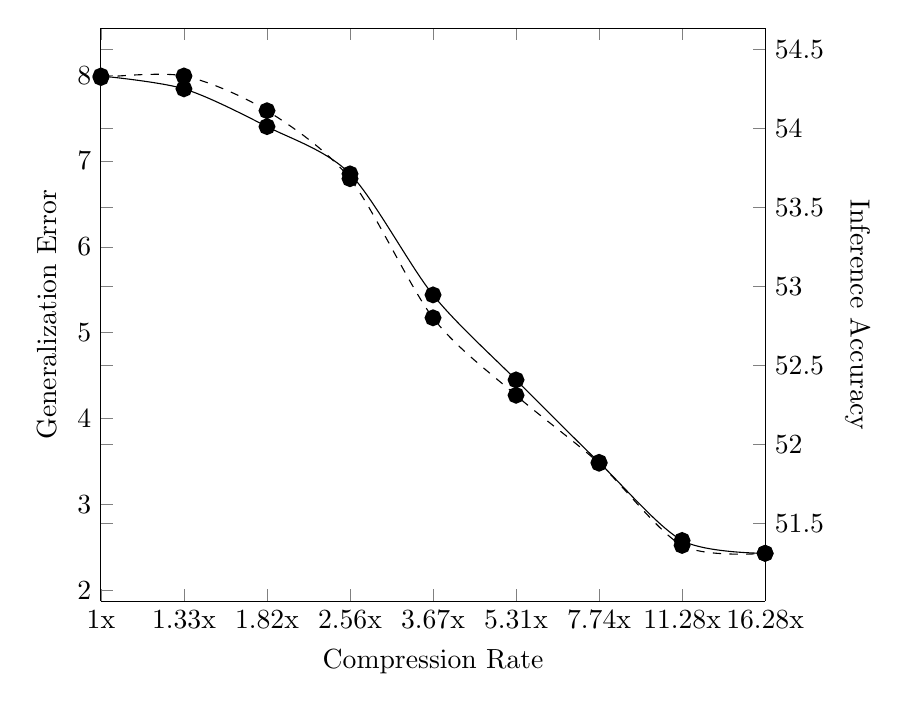
\begin{tikzpicture}
% let both axes use the same layers
\pgfplotsset{set layers}
%
\begin{axis}[
scale only axis,
line width=2.0pt,
mark size=2.0pt,
xmin=0,xmax=8,
ylabel={Generalization Error},
axis y line*=left,
xlabel={Compression Rate},
xtick={0,1,2,3,4,5,6,7,8},
xticklabels={1x, 1.33x, 1.82x, 2.56x, 3.67x, 5.31x, 7.74x, 11.28x, 16.28x}
]
\addplot[
    color=black,
    solid,
    mark=*,
    mark options={solid},
    smooth
    ]
    coordinates {
    (0,7.99)(1,7.84)(2,7.4)(3,6.85)(4,5.44)(5,4.45)(6,3.49)(7,2.58)(8,2.43)
      };
\end{axis}

\begin{axis}[
scale only axis,
line width=2.0pt,
mark size=2.0pt,
xmin=0,xmax=8,
ylabel near ticks, yticklabel pos=right,
ylabel={Inference Accuracy},
ylabel style = {rotate=180},
axis x line=none
]
\addplot[
    color=black,
    dashed,
    mark=*,
    mark options={solid},
    smooth
    ]
    coordinates {
    (0,54.32)(1,54.33)(2,54.11)(3,53.68)(4,52.80)(5,52.31)(6,51.88)(7,51.36)(8,51.31)
        };
\end{axis}
\end{tikzpicture} &

%
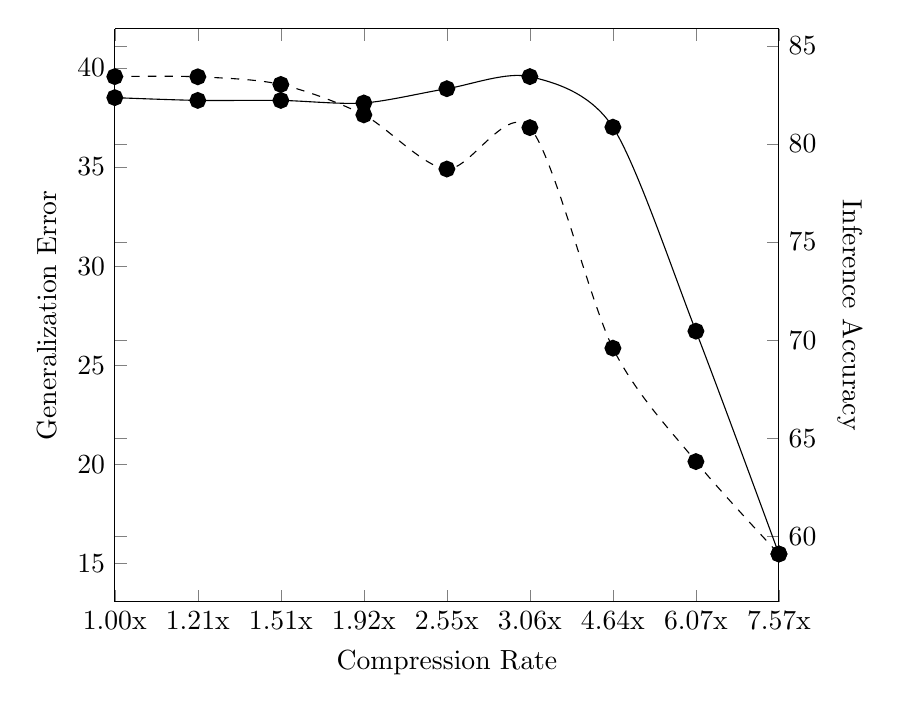
\begin{tikzpicture}
% let both axes use the same layers
\pgfplotsset{set layers}
%
\begin{axis}[
scale only axis,
line width=2.0pt,
mark size=2.0pt,
xmin=0,xmax=8,
ylabel={Generalization Error},
axis y line*=left,
xlabel={Compression Rate},
xtick={0,1,2,3,4,5,6,7,8},
xticklabels={1.00x, 1.21x, 1.51x, 1.92x, 2.55x, 3.06x, 4.64x, 6.07x, 7.57x}
]
\addplot[
    color=black,
    solid,
    mark=*,
    mark options={solid},
    smooth
    ]
    coordinates {
    (0,38.5)(1,38.36)(2,38.36)(3,38.23)(4,38.95)(5,39.56)(6,37.01)(7,26.72)(8,15.48)
      };
\end{axis}

\begin{axis}[
scale only axis,
line width=2.0pt,
mark size=2.0pt,
xmin=0,xmax=8,
ylabel near ticks, yticklabel pos=right,
ylabel={Inference Accuracy},
ylabel style = {rotate=180},
axis x line=none
]
\addplot[
    color=black,
    dashed,
    mark=*,
    mark options={solid},
    smooth
    ]
    coordinates {
    (0,83.43)(1,83.42)(2,83.03)(3,81.48)(4,78.72)(5,80.83)(6,69.59)(7,63.81)(8,59.10)
        };
\end{axis}
\end{tikzpicture} &





%
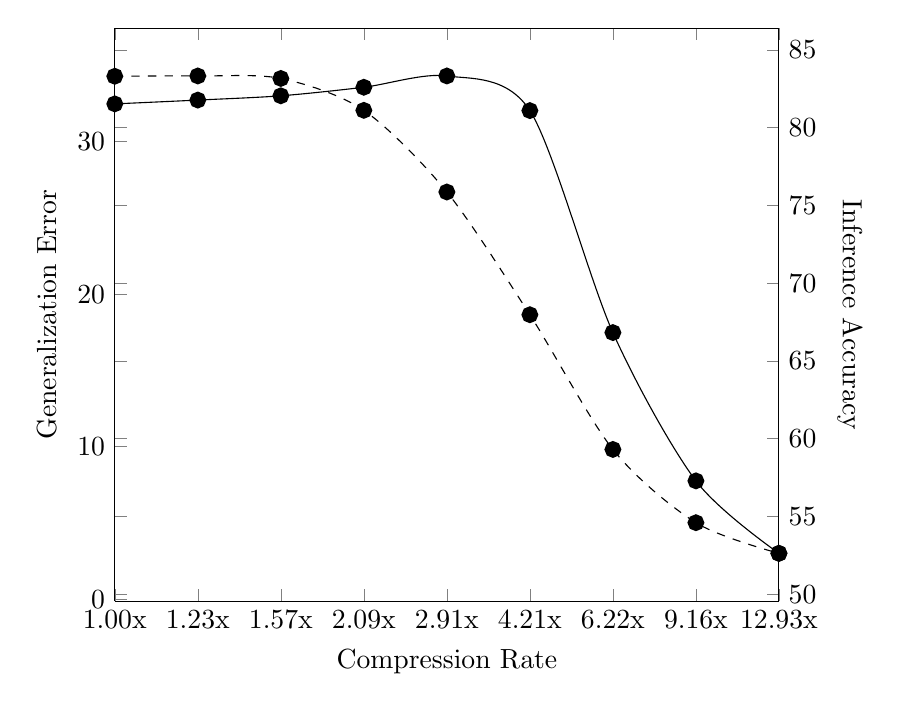
\begin{tikzpicture}
% let both axes use the same layers
\pgfplotsset{set layers}
%
\begin{axis}[
scale only axis,
line width=2.0pt,
mark size=2.0pt,
xmin=0,xmax=8,
ylabel={Generalization Error},
axis y line*=left,
xlabel={Compression Rate},
xtick={0,1,2,3,4,5,6,7,8},
xticklabels={1.00x, 1.23x, 1.57x, 2.09x, 2.91x, 4.21x, 6.22x, 9.16x, 12.93x}
]
\addplot[
    color=black,
    solid,
    mark=*,
    mark options={solid},
    smooth
    ]
    coordinates {
    (0,32.47)(1,32.72)(2,33)(3,33.56)(4,34.3)(5,32.03)(6,17.48)(7,7.76)(8,3.01)
      };
\end{axis}

\begin{axis}[
scale only axis,
line width=2.0pt,
mark size=2.0pt,
xmin=0,xmax=8,
ylabel near ticks, yticklabel pos=right,
ylabel={Inference Accuracy},
ylabel style = {rotate=180},
axis x line=none
]
\addplot[
    color=black,
    dashed,
    mark=*,
    mark options={solid},
    smooth
    ]
    coordinates {
    (0,83.30)(1,83.32)(2,83.16)(3,81.11)(4,75.86)(5,67.97)(6,59.31)(7,54.60)(8,52.63)
        };
\end{axis}
\end{tikzpicture}


\end{tabular}
}
\caption{FashionMNIST(left) Purchase100(Center) Location(Right). Dashed is Inference accuracy, solid is generalisaton error}
\label{fig:loss}
\end{center}
\end{figure*}

\begin{figure*}[ht!]
\begin{center}% note that \centering uses less vspace...
\resizebox{2\columnwidth}{!}{%
\begin{tabular}{lllll}


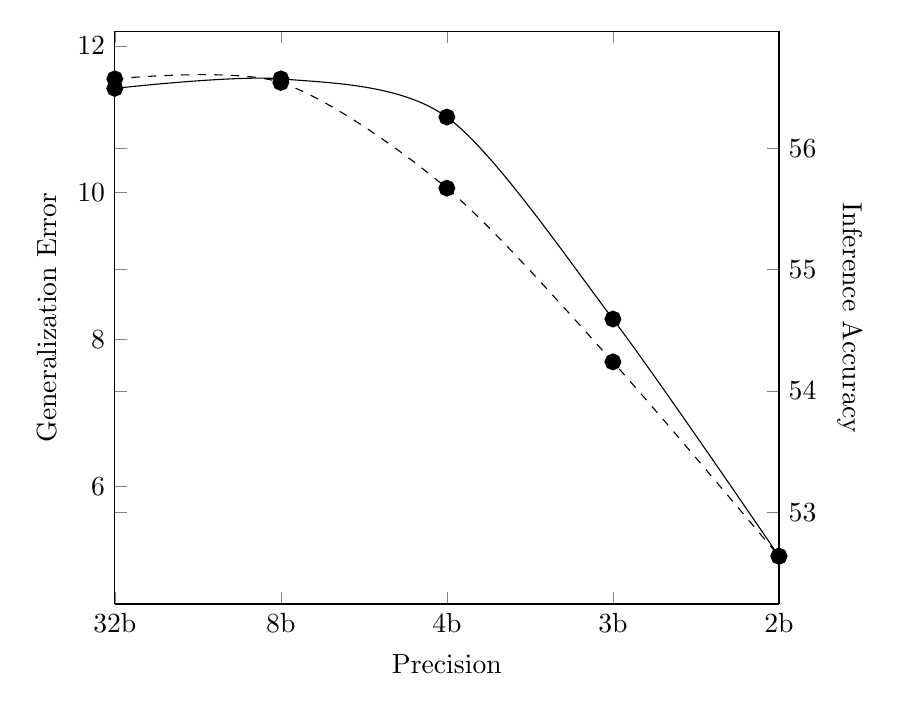
\begin{tikzpicture}
% let both axes use the same layers
\pgfplotsset{set layers}
%
\begin{axis}[
scale only axis,
line width=2.0pt,
mark size=2.0pt,
xmin=0,xmax=4,
ylabel={Generalization Error},
axis y line*=left,
xlabel={Precision},
xtick={0,1,2,3,4},
xticklabels={32b, 8b, 4b, 3b, 2b}
]
\addplot[
    color=black,
    solid,
    mark=*,
    mark options={solid},
    smooth
    ]
    coordinates {
    (0,11.42)(1,11.55)(2,11.03)(3,8.28)(4,5.05)
      };
\end{axis}

\begin{axis}[
scale only axis,
line width=2.0pt,
mark size=2.0pt,
xmin=0,xmax=4,
ylabel near ticks, yticklabel pos=right,
ylabel={Inference Accuracy},
ylabel style = {rotate=180},
axis x line=none
]
\addplot[
    color=black,
    dashed,
    mark=*,
    mark options={solid},
    smooth
    ]
    coordinates {
    (0,56.57)(1,56.54)(2,55.67)(3,54.24)(4,52.64)
        };
\end{axis}
\end{tikzpicture} &

%
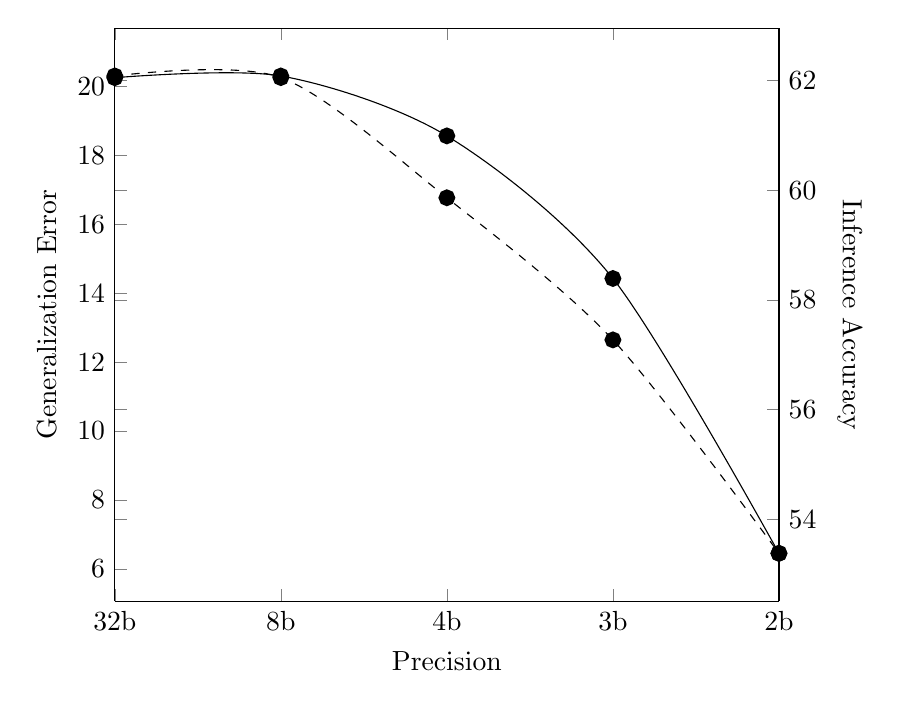
\begin{tikzpicture}
% let both axes use the same layers
\pgfplotsset{set layers}
%
\begin{axis}[
scale only axis,
line width=2.0pt,
mark size=2.0pt,
xmin=0,xmax=4,
ylabel={Generalization Error},
axis y line*=left,
xlabel={Precision},
xtick={0,1,2,3,4},
xticklabels={32b, 8b, 4b, 3b, 2b}
]
\addplot[
    color=black,
    solid,
    mark=*,
    mark options={solid},
    smooth
    ]
    coordinates {
    (0,20.26)(1,20.31)(2,18.57)(3,14.43)(4,6.45)
      };
\end{axis}

\begin{axis}[
scale only axis,
line width=2.0pt,
mark size=2.0pt,
xmin=0,xmax=4,
ylabel near ticks, yticklabel pos=right,
ylabel={Inference Accuracy},
ylabel style = {rotate=180},
axis x line=none
]
\addplot[
    color=black,
    dashed,
    mark=*,
    mark options={solid},
    smooth
    ]
    coordinates {
    (0,62.08)(1,62.05)(2,59.86)(3,57.27)(4,53.38)
        };
\end{axis}
\end{tikzpicture} &





%
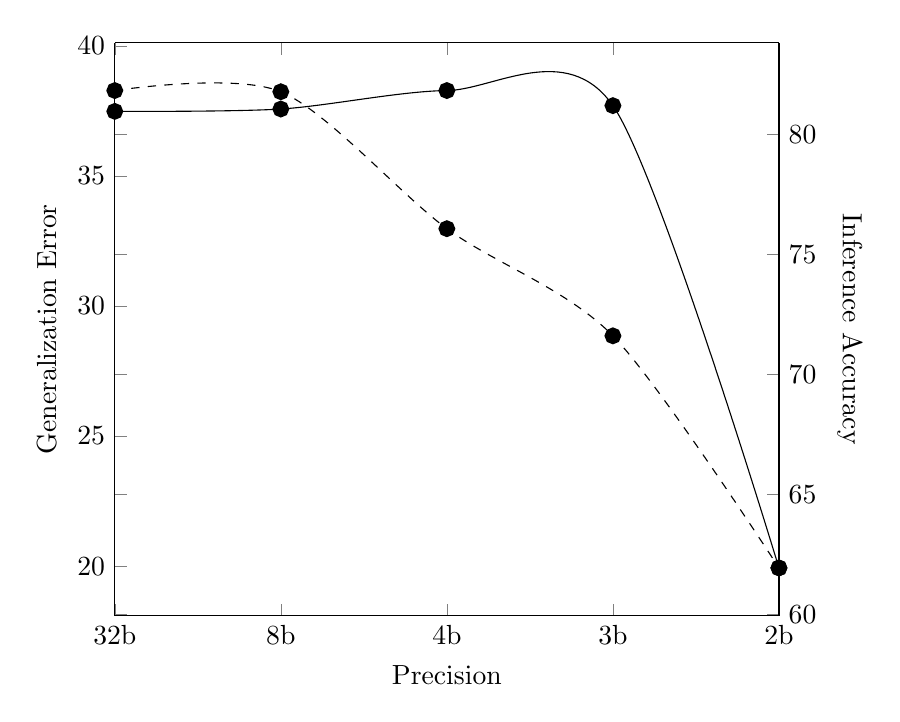
\begin{tikzpicture}
% let both axes use the same layers
\pgfplotsset{set layers}
%
\begin{axis}[
scale only axis,
line width=2.0pt,
mark size=2.0pt,
xmin=0,xmax=4,
ylabel={Generalization Error},
axis y line*=left,
xlabel={Precision},
xtick={0,1,2,3,4},
xticklabels={32b, 8b, 4b, 3b, 2b}
]
\addplot[
    color=black,
    solid,
    mark=*,
    mark options={solid},
    smooth
    ]
    coordinates {
    (0,37.48)(1,37.57)(2,38.28)(3,37.70)(4,19.93)
      };
\end{axis}

\begin{axis}[
scale only axis,
line width=2.0pt,
mark size=2.0pt,
xmin=0,xmax=4,
ylabel near ticks, yticklabel pos=right,
ylabel={Inference Accuracy},
ylabel style = {rotate=180},
axis x line=none
]
\addplot[
    color=black,
    dashed,
    mark=*,
    mark options={solid},
    smooth
    ]
    coordinates {
    (0,81.82)(1,81.77)(2,76.07)(3,71.61)(4,61.95)
        };
\end{axis}
\end{tikzpicture}


\end{tabular}
}
\caption{\underline{Pruning followed by Weight Sharing (Quantization).} While the retraining after pruning is necessary to restore the predictive accuracy, clustering the weights to reduce the precision lowers the inference accuracy (dashed line) risk while reducing the generalization error (solid line) for FashionMNIST(left), Purchase100(Center) and Location(Right) dataset.}
\label{fig:loss}
\end{center}
\end{figure*}


\noindent\textbf{Computation Efficiency.} Design of efficient off-the-shelf architectures replaces the complex matrix-vector multiplications by multiple matrix-vector multiplications with smaller dimensions.
This reduces the overall number of parameters but it has been shown empirically\footnote{https://github.com/albanie/convnet-burden} that this does not necessarily reduce the number of multiply accumulate operations or FLOPS~\cite{article}.
In case of parameter pruning, achieving efficiency requires additional hardware optimization. Particularly, instead of actually computing the the multiplications with "0"pruned values, the hardware optimization enable the user to skip the computation and replace the output by a "0" directly.
For quantized models with binarized parameters and activations the MAC operations can be replaced by binary operations such as XNOR and the maxpool operations can be replaced by OR operation, while the activations can be replaced by checking the parity bit (denotes the sign) operation and hence reducing the FLOPS drastically[XONN].
This results in high computational efficiency and hence, faster inference.


\noindent\textbf{Energy Efficiency.} Energy efficiency has been shown to not vary much in case of reduction with number of parameters and data type, number of memory accesses play vital role[CVPR 2017 yang et al][].
Specifically, for the case of off-the-shelf architectures the while the computation efficiency has been shown to improve, the energy efficiency has been shown to be close to large scale state of the art models like AlexNet[suqeezenet][].
Alternatively, for the case of model compression, energy efficiency can be achieved by additionally providing hardware optimization and shows small improvement in the energy consumption[].
For quantization, however, the energy efficiency has been shown to be high [][] where the memory access can be drastically reduced by increasing the throughput of data fetched from the memory.
Specifically, lowering the precision from 32 bit floating point to binary results in lowering the memory accesses and 32x improvement in energy consumption[][][].
While some improvement is seen natively for quantized models (from replacing MACs with XNOR), higher benefits can be achieved via additional hardware optimization[].
The benchmarking of energy consumption for different optimization and architectures is well explored in the literature and out of scope of this work. We refer the authors to [][][] for more details.

In summary, compared to different optimization techniques for NNs, the quantized architectures show significant benefit for different efficiency requirements over the other alternatives.


\subsection{Evaluating Privacy Leakage}

In this section, we evaluate the information leakage through membership inference attacks for the three baseline algorithms considered.
This is the main contribution of our work where we evaluate the privacy leakage for different optimization and design algorithms for NNs.

\subsubsection{Model Compression}

We evaluate the privacy leakage on compressing a model by pruning the connections in the model.
Here, pruning is achieved by replacing some of the parameters with "0" value.
As described in the original paper~\cite{}, pruning is followed by retraining the model to restore the model's original accuracy with the pruned connections.

We evaluate and validate the impact on membership privacy on compressing the model trained on three datasets: FashionMNIST, Location and Purchase100.
On pruning the model, the model's test accuracy decreases but also lowers the membership inference accuracy (Figure~\ref{fig:prune}).
This is expected as the parameters are responsible for memorizing the training data information and pruning the parameters lowers the adversary's attack success~\cite{rezawhite}.

However, interestingly, on retraining the pruned model, we observe that the membership inference accuracy is much higher than the original unpruned baseline model (Figure~\ref{fig:retrain}).
This indicates that model compression in turn increases the overall privacy leakage.
This can be attributed to the lower number of parameters forced to learn the same amount of information stored previously in the unpruned model with larger number of parameters.
In other words, the same amount of information is now captured by less number of parameters resulting in higher memorization of information per parameter.
To analyze the information stored per parameter, we first compute the model capacity as the mutual information of a trained network between the true label $Y$ and the predicted label $Y_{\theta}$ for a random input $X$ as derived in~\cite{45932,cap}.
Here, model's information $I(Y;Y_{\theta}|X) = $
\begin{equation}
N_{train}\left(1 - (r_{train}log_2(\frac{1}{r_{train}}) + (1-r_{train})log_2(\frac{1}{1-r_{train}}))\right)
\end{equation}
where $r_{train}$ is the classification train accuracy for all the $N_{train}$ samples in the training data.
For $r_{train} = 1$, the model completely memorizes all random samples as the information stored equals the number of samples $N_{train}$, while for $r_{train}=0.5$, the training accuracy 0.
We divide the above equation by the model's total number of parameters $N_{param}$ to get the per parameter information stored as
\begin{equation}
I_p(Y;Y_{\theta}|X) = \frac{I(Y;Y_{\theta}|X)}{N_{param}}
\end{equation}
As the model is compressed (pruned), the number of parameters $N_{param}$ decreases which results in increase in $I_p(Y;Y_{\theta}|X)$. However, on aggressive pruning, the train accuracy $r_{train}$ also decreases resulting in a decrease in the information per parameter, which is empirically indicated by a decrease in membership inference accuracy at the end in Figure~\ref{fig:retrain}.


\textbf{Mitigating the Privacy Risks in Pruned Models.} We describe on potential approach to mitigate the privacy risk of the compressed models without requiring to modify the model's training.
The post-hoc apporach utilizes the weight sharing for the compressed model. This is however, accompanied by a decrease in the model's prediction accuracy indicating a privacy-utility trade-off.
As seen in Figure~\ref{fig:wtsharing}, reducing the precision from 32 bits to 2 bits results in a decrease in inference accuracy from 56.57\% to 52.64\% for FashionMNIST, 62.08\% to 53.38\% for Location and 81.82\% to 61.95\% for Purchase100 dataset.
This decrease in inference attack accuracy is closely followed by a decrease in generalization error which is indicative of decrease in prediction accuracy of the model.
We evaluate the effectiveness of pruning followed by quantization which has been shown to have significant impact on reducing the model complexity through compression more significantly than either pruning or quantization alone.
For the experiments, we use the compressed model indicating highest privacy leakage to evaluate the effectiveness of weight sharing on the worst case condition.
This pipelined approach of pruning followed by retraining followed by weight sharing, not only maintains the algorithm's objective for efficiency but is used as a post-hoc approach to reduces the overall inference risk~\cite{DBLP:journals/corr/HanMD15,DBLP:journals/corr/HanPNMTECTD16}.






\subsubsection{Off-the-Shelf Efficient Architectures}


\begin{table}[!htb]
\begin{center}
\renewcommand\arraystretch{1.5}
\fontsize{6.7pt}{6.7pt}\selectfont
\begin{tabular}{|c|c|c|c|c|}
\hline
\textbf{Architecture} & \textbf{Memory} & \textbf{Train}  & \textbf{Test}  & \textbf{Inference}   \\
 & \textbf{Footprint} & \textbf{Accuracy} & \textbf{Accuracy} & \textbf{Accuracy}  \\
\hline
SqueezeNet & 5 MB & 88.21\% & 81.92\% & \cellcolor{green!25}53.07\% \\
MobileNetV2 & 14 MB & 97.50\% & 87.24\% & \cellcolor{green!25}55.57\% \\
\hline
AlexNet & 240 MB & 97.86\% & 80.34\% & \cellcolor{red!25}60.40\% \\
VGG11 & 507 MB & 99.13\% & 86.43\% & \cellcolor{red!25}58.04\% \\
VGG16 & 528 MB & 99.58\% & 88.95\% & \cellcolor{red!25}58.70\%  \\
VGG19 & 549 MB & 99.09\% & 88.18\% & \cellcolor{red!25}57.85\% \\
\hline
\end{tabular}
\end{center}
\caption{Model complexity influences the membership inference leakage. Model specifically designed for efficiency leak less information.}
\label{stdarch}
\end{table}

In this section, we evaluate two popular state of the art architectures, SqueezeNet and MobileNet, trained on CIFAR10 dataset used for low powered systems.
As seen in Table~\ref{stdarch}, the SqueezeNet and MobileNet models shows lower inference accuracy of 53.07\% and 55.57\% compared to larger models which have higher privacy leakage.

\begin{figure}[hb!]
\resizebox{0.8\columnwidth}{!}{%
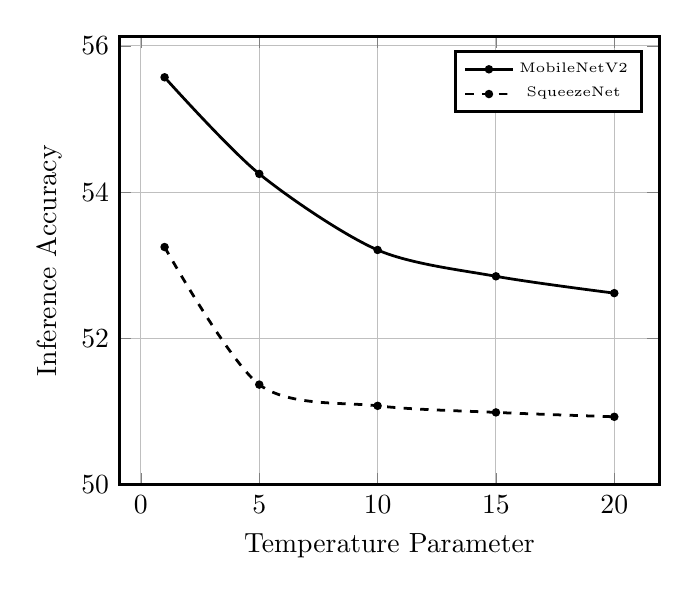
\begin{tikzpicture}
\begin{axis}[
legend style={font=\tiny},
legend pos =  north east,
line width=1.0pt,
mark size=1.0pt,
ymin=50,
legend entries={MobileNetV2, SqueezeNet},
ylabel={Inference Accuracy},
xlabel={Temperature Parameter},
% extra x ticks={1,10,...,400},
% extra y ticks={0,0.5,...,10},
% extra y tick labels={},
% extra x tick labels={},
% extra x tick style={grid=major},
% extra y tick style={grid=major},
grid=major
]
\addplot[
    color=black,
    solid,
    mark=*,
    mark options={solid},
    smooth
    ]
    coordinates {
    (1,55.57)(5,54.25)(10,53.21)(15,52.85)(20,52.62)
      };
\addplot[
      color=black,
      dashed,
      mark=*,
      mark options={solid},
      smooth
    ]
    coordinates {
    (1,53.25)(5,51.37)(10,51.08)(15,50.99)(20,50.93)
      };
\end{axis}
\end{tikzpicture}
}
\caption{The privacy leakage of models designed for efficiency (SqueezeNet and MobileNet) can be reduced by increasing the softmax temperature. }
\end{figure}


Further, the inference accuracy of SqueezeNet and MobileNet can be further reduced close to random guess by increasing the temperature parameter of the softmax function applied to the output.
Increasing the temperature parameter reduces the granularity of the model's output and is given by $F_i(x) = \frac{e^{\frac{z_i(x)}{T}}}{\sum_{j}e^{\frac{z_j(x)}{T}}}$ where $z(x)$ computes output of the model before the softmax layer.
For the case of SqueezeNet, we are able to reduce the inference accuracy to 50.93\% from 53.07\% while for MobileNet we can reduce the inference accuracy to 52.62\% from 55.57\% as seen in Figure~\ref{softmax}.
This reduction in inference accuracy is without any cost of the prediction test accuracy of the model.




\subsubsection{Quantization}

In this section, we evaluate the technique of reducing the precision of both model's parameters and intermediate activations.
Further, we consider the extreme case of binarizing the parameters and activations allowing to evaluate on the most optimized case.
We evaluate on FashionMNIST dataset for two architectures with convolutional and fully connected layers.

\begin{table}[!htb]
\begin{center}
\renewcommand\arraystretch{1.5}
\fontsize{6.7pt}{6.7pt}\selectfont
\begin{tabular}{|c|c|c|c|c|}
\hline
\multicolumn{5}{|c|}{\textbf{FashionMNIST}}\\
\hline
\textbf{Architecture} & \textbf{Memory} & \textbf{Train}  & \textbf{Test}  & \textbf{Inference}  \\
 & \textbf{Accuracy} &  \textbf{Footprint} & \textbf{Accuracy} & \textbf{Accuracy}  \\
\hline
\multicolumn{5}{|c|}{Architecture 1}\\
Full & 38.39 MB & 100\% & 92.35\% & \cellcolor{red!25}57.46\%\\
BinaryNet & 1.62 MB & 88.68\% & 86.9\% & \cellcolor{green!25}55.45\%\\
XNOR-Net & 1.62 MB & 87.19\% & 85.68\% & \cellcolor{green!25}51.05\%\\ %1,626,824 parameters
\hline
\multicolumn{5}{|c|}{Architecture 2}\\
Full & 29.83 MB & 99.34\% & 89.88\% & \cellcolor{red!25}54.86\% \\
BinaryNet & 0.93 MB & 97.61\% & 89.60\% & \cellcolor{green!25}54.30\%\\
XNOR-Net & 0.93 MB & 92.67\% & 86.68\% & \cellcolor{green!25}51.74\%\\ %937,000parameters
\hline
\end{tabular}
\end{center}
\caption{Reducing the model precision lowers the inference attack accuracy but at the cost of test accuracy.}
\label{fmnist_quantize}
\end{table}

In both the architectures, we see that computation on  binarized parameters and activations reduces the inference risk by a small value.
However, on replacing the MAC operations with XNOR operations, we observe that the inference risk decreases close to random guess, however, at the cost of prediction test accuracy.

In summary, we observe that quantization, specifically binarization of parameters and activation along with XNOR computation, provides strong resistance against inference attacks compared to model compression and off-the-shelf architectures.

\subsection{Summary of Comparison}

We summarize the properties satisfied by each of the technique in terms of privacy, computation, memory and energy efficiency in Table~\ref{tbl:comparison}.
Here, we mark the attributes which are satisfied with $\cmark$, requires additional hardware optimization as $\smark$ and does not satisfy the property with a $\xmark$.

\begin{table}[!htb]
\begin{center}
\renewcommand\arraystretch{1.5}
\fontsize{6.7pt}{6.7pt}\selectfont
\begin{tabular}{|l||l|l|l|}
\hline
Requirements & Compression & Quantization & Off-the-shelf  \\
\hline
Computation Efficiency & $\smark$  & $\cmark$   & $\xmark$ \\
\hline
Memory Efficiency &  $\smark$ & $\cmark$   & $\cmark$ \\
\hline
Energy Efficiency &  $\smark$   & $\cmark$   & $\xmark$ \\
\hline
Privacy &  $\xmark$   & $\cmark$   & $\smark$ \\
\hline
\end{tabular}
\end{center}
\caption{Comparison of different optimizations for NNs. $\smark$: additional hardware optimization; $\xmark$: requirement not satisfied; $\cmark$: requirement satisfied.}
\label{tbl:comparison}
\end{table}

For our requirement, quantization of NNs is an attractive design choice which not only satisfies the computation, memory and energy efficiency but also provides high resistance against inference attacks.
Specifically, in this work we only consider the aggressive quantization of binarizing the parameters and activations to \{-1,+1\} values while additionally replacing the MAC operations with cheap and efficient binary arithmetic (XNOR operations).
Hence, we choose this particular design for NNs to provide a good three dimensional trade-off between privacy-efficiency-accuracy.

\section{Evaluation}
\label{compare}

We carried out an extensive evaluation of \method.
We first analyse the three state of the art techniques for efficiency model computation in Section~\ref{eval-efficiency} and privacy leakage in Section~\ref{eval-leakage}, before summarizing the comparison Section~\ref{eval-summary}.
We then evaluate the proposed training methodology in Section~\ref{evalPh1} and Section~\ref{evalPh2} for Phase I and Phase II, respectively.
Finally, we compare \method~ against state of the art defence schemes in Section~\ref{eval-defences}.


\subsection{Evaluating Efficiency}
\label{eval-efficiency}

In this section, in the view of the memory-computation-energy efficiency requirements, we compare the three baseline algorithms (i.e., model compression, off-the-shelf architecture, and quantization).
%We then select an efficient design scheme for NNs that satisfies all our requirements.


\noindent\textbf{Memory Efficiency.} Off the shelf models are designed to specifically reduce the memory footprint.
For instance, the memory footprint of Squeezenet and MobileNet is 5MB and 14Mb compared to 250Mb of Alexnet and >500Mb of VGG architectures~\cite{DBLP:journals/corr/IandolaMAHDK16,conf/cvpr/SandlerHZZC18}.
Additionally, lowering the model precision from 64 or 32 bit floating point to binary precision results in a direct reduction of 64x or 32x in the overall memory footprint of the model.
However, in case of model compression the model parameters which are pruned are simply replaced by a value of "0".
Hence, storing even the "0" parameter takes up memory and does not necessarily decrease the overall memory footprint unless the hardware is optimized to skip the storage of all the zero values in the memory.
This requires additional logic to check for zero valued parameters in a dictionary.


\noindent\textbf{Computation Efficiency.} Design of efficient off-the-shelf architectures replaces the complex matrix-vector multiplications to smaller dimensions.
This reduces the overall number of parameters but it has been shown empirically\footnote{https://github.com/albanie/convnet-burden} that this does not necessarily reduce the number of multiply accumulate operations~\cite{article}.
In case of parameter pruning, achieving efficiency requires additional hardware optimization. Particularly, instead of actually computing the multiplications with "0" pruned values, the hardware optimization enables the user to skip the computation and replace the output by a "0" directly.
For quantized models with binarized parameters and activations the MACs can be replaced by binary XNOR operations, maxpool replaced by OR operation, while the activations can be replaced by checking the sign bit and hence reducing the FLOPS drastically~\cite{235489}.
This results in high computational efficiency and hence, faster inference.

\begin{figure*}[!htb]
    \centering

\subfloat[Impact of Model Pruning on Privacy (FashionMNIST)]{\label{fig:prune}{
  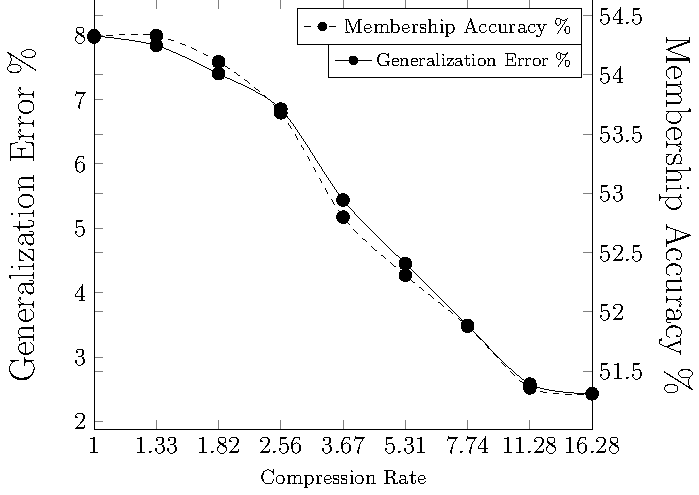
\includegraphics[width=0.28\linewidth]{figures/fmnist_prune.pdf}}}
\hspace{4mm}
\subfloat[Impact of Retraining on Privacy]{\label{fig:retrain}{
  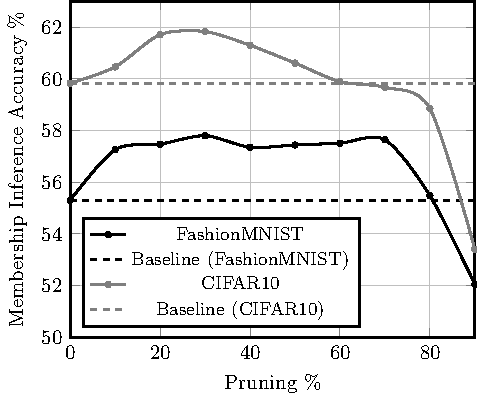
\includegraphics[width=0.28\linewidth]{figures/retrain.pdf}}}
\hspace{4mm}
\subfloat[Mitigating Privacy Leakage via Weight Sharing (FashionMNIST)]{\label{fig:wtsharing}{
  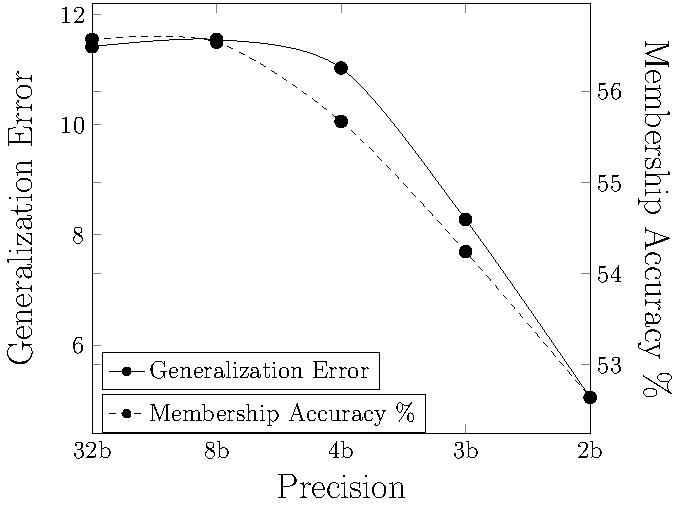
\includegraphics[width=0.28\linewidth]{figures/fmnist_wtsharing.pdf}}}
    \caption{Pruning the model lowers the membership inference leakage at the cost of accuracy. Retraining the pruned model to restore accuracy results in a higher membership privacy leakage compared to uncompressed baseline model. This additional leakage can be mitigated by weight sharing at the cost of accuracy.}
    \label{fig:NIAcause}
\end{figure*}



\noindent\textbf{Energy Efficiency.} Energy efficiency does not vary much with reduction of number of parameters and data type, but the number of memory accesses play vital role~\cite{6757323}.
Specifically, for the case of off-the-shelf architectures, while computation efficiency improves, the energy efficiency is close to large scale state of the art models like AlexNet~\cite{DBLP:journals/corr/IandolaMAHDK16,8114708}.
Alternatively, for the case of model compression, energy efficiency can be marginally improved by additionally providing hardware optimization~\cite{journals/corr/YangCS16a,DBLP:journals/corr/HanMD15}.
For quantization, however, the energy efficiency is high as the memory access can be drastically reduced by increasing the throughput of data fetched from the memory.
Specifically, lowering the precision from 32 bit floating point to binary results in lowering the memory accesses and 32x improvement in energy consumption~\cite{NIPS2016_6573,rastegari2016xnornet}.
While some improvements are seen natively for quantized models (from replacing MACs with XNOR), higher benefits can be achieved via additional hardware optimization~\cite{Umuroglu2017FINNAF}.
The benchmarking of energy consumption for different optimization and architectures is well explored in the literature and out of scope of this work. We refer the readers to~\cite{8114708} for more details.

In summary, compared to different optimization techniques, the quantized architectures show significant benefits for different efficiency requirements over the other alternatives.
% for NNs



\subsection{Evaluating Privacy Leakage}
\label{eval-leakage}

In this section, we evaluate the information leakage through membership inference attacks for the three baseline algorithms considered.
This is the main contribution of our work where we evaluate the privacy leakage for different optimization and design algorithms for NNs.

\subsubsection{Model Compression}

We evaluate the privacy leakage on compressing a model by pruning the connections in the model.
Here, pruning is achieved by replacing some of the parameters with "0" value.
As described in the original paper~\cite{Han:2015:LBW:2969239.2969366,DBLP:journals/corr/HanPNMTECTD16}, pruning is followed by retraining the model to restore the model's original accuracy with the pruned connections.
We evaluate and validate the impact on membership privacy on compressing the model trained on two datasets: FashionMNIST and CIFAR10.

\textbf{Impact of Pruning Parameters.} On pruning the model, the model's test accuracy decreases but also lowers the membership inference accuracy (Figure~\ref{fig:prune}). % for FashionMNIST
As the compression rate increases, the generalization error decreases (owing to a decrease in both train and test accuracy) with a decrease in membership accuracy to close to random guess.
This is expected as the parameters are responsible for memorizing the training data information~\cite{DBLP:journals/corr/abs-1812-00910,236216,10.1145/3133956.3134077} and pruning the parameters lowers the adversary's attack success.




%\begin{figure}[!htb]
%    \centering
%    \begin{minipage}[b]{1\linewidth}
%    \centering
%    \subfigure[Impact of Model Pruning on Privacy]{
%    \label{fig:prune}
%    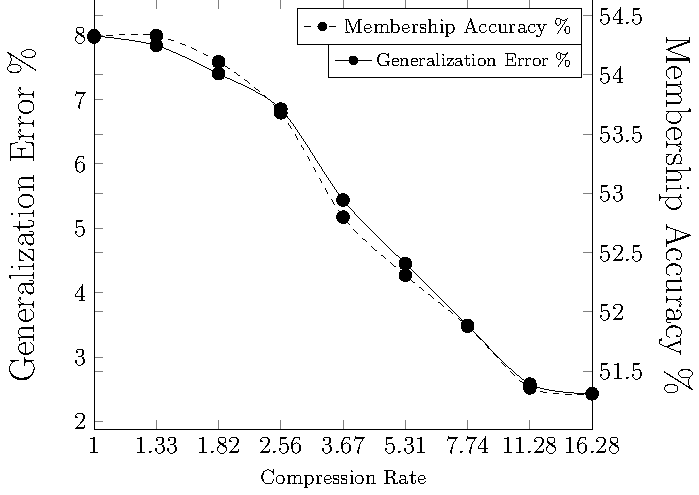
\includegraphics[width=0.7\linewidth]{figures/fmnist_prune.pdf}
%    }
%    \subfigure[Impact of Retraining on Privacy]{
%    \label{fig:retrain}
%    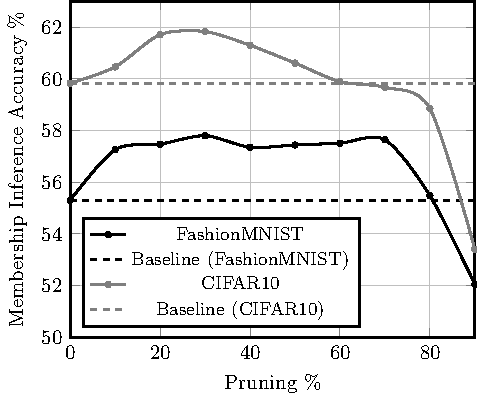
\includegraphics[width=0.7\columnwidth]{figures/retrain.pdf}
%    }
%    \subfigure[Mitigating Privacy Leakage via Weight Sharing]{
%    \label{fig:wtsharing}
%    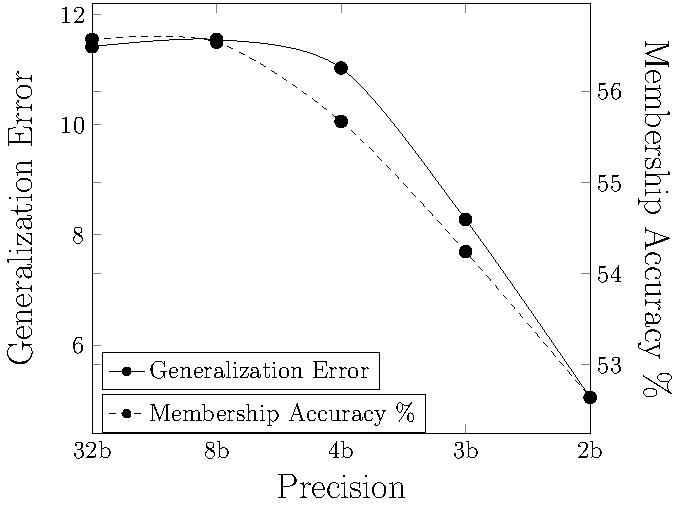
\includegraphics[width=0.7\linewidth]{figures/fmnist_wtsharing.pdf}
%    }
%
%    \end{minipage}
%    \caption{Pruning the model lowers the membership inference leakage at the cost of accuracy. Retraining the pruned model to restore accuracy results in a higher membership privacy leakage compared to uncompressed baseline model. This additional leakage can be mitigated by weight sharing at the cost of accuracy.}
%    \label{fig:NIAcause}
%\end{figure*}


\textbf{Impact of Retraining Pruned Model.} Interestingly, on retraining the pruned model, we observe that the membership inference accuracy is much higher than the original unpruned baseline model (Figure~\ref{fig:retrain}).
This indicates that model compression in turn increases the overall privacy leakage.
This can be attributed to the lower number of parameters forced to learn the same amount of information stored previously in the unpruned model with larger number of parameters.
In other words, the same amount of information is now captured by less number of parameters resulting in higher memorization of information per parameter.
As the model is compressed (pruned), the number of parameters decreases which results in increase in information per parameter. However, on aggressive pruning, the train and test accuracy also decreases resulting in a decrease in the information per parameter, which is empirically indicated by a decrease in membership inference accuracy at the end in Figure~\ref{fig:retrain}.

%To analyze the information stored per parameter, we first compute the model capacity as the mutual information of a trained network between the true label $Y$ and the predicted label $Y_{\theta}$ for a random input $X$ as derived in~\cite{45932,cap}.
%Here, model's information $I(Y;Y_{\theta}|X) = $
%\begin{equation}
%\footnotesize
%N_{train}\left(1 - (r_{train}log_2(\frac{1}{r_{train}}) + (1-r_{train})log_2(\frac{1}{1-r_{train}}))\right)
%\end{equation}
%where $r_{train}$ is the classification train accuracy for all the $N_{train}$ samples in the training data.
%For $r_{train} = 1$, the model completely memorizes all random samples as the information stored equals the number of samples $N_{train}$, while for $r_{train}=0.5$, the training accuracy 0.
%We divide the above equation by the model's total number of parameters $N_{param}$ to get the per parameter information stored as
%\begin{equation}
%I_p(Y;Y_{\theta}|X) = \frac{I(Y;Y_{\theta}|X)}{N_{param}}
%\end{equation}

In summary, model compression results in a higher membership privacy leakage compared to the baseline uncompressed model making it a poor candidate for applications with sensitive data.

\textbf{Mitigating the Privacy Risks in Pruned Models.} We describe on potential approach to mitigate the privacy risk of the compressed models without requiring to modify the model's training.
The post-hoc approach utilizes the weight sharing (a class of quantization techniques) for the compressed model. This is however, accompanied by a decrease in the model's prediction accuracy indicating a privacy-utility trade-off.
As seen in Figure~\ref{fig:wtsharing}, reducing the precision from 32 bits to 2 bits results in a decrease in inference accuracy from 56.57\% to 52.64\% for FashionMNIST.
This decrease in inference attack accuracy is caused by a decrease in generalization error due to decrease in prediction (both train and test) accuracy of the model.
For the experiments, we use the compressed model with highest privacy leakage (by sweeping sensitivity threshold values) to evaluate the effectiveness of weight sharing on the worst case condition. % in case of FashionMNIST 
This pipeline approach of pruning followed by retraining followed by weight sharing, not only maintains the algorithm's objective for efficiency but is used as a post-hoc approach to reduces the overall inference risk~\cite{DBLP:journals/corr/HanMD15,DBLP:journals/corr/HanPNMTECTD16}.






\subsubsection{Off-the-Shelf Efficient Architectures}


\begin{table}[h]
\begin{center}
\renewcommand\arraystretch{1.5}
\fontsize{6.5pt}{6.5pt}\selectfont
\begin{tabular}{|c|c|c|c|c|}
\hline
\multicolumn{5}{|c|}{\textbf{CIFAR10}}\\
\hline
\textbf{Architecture} & \textbf{Memory} & \textbf{Train}  & \textbf{Test}  & \textbf{Inference}   \\
 & \textbf{Footprint} & \textbf{Accuracy} & \textbf{Accuracy} & \textbf{Accuracy}  \\
\hline
SqueezeNet & 5 MB & 88.21\% & 81.92\% & \cellcolor{green!25}53.07\% \\
MobileNetV2 & 14 MB & 97.50\% & 87.24\% & \cellcolor{green!25}55.57\% \\
\hline
AlexNet & 240 MB & 97.86\% & 80.34\% & \cellcolor{red!25}60.40\% \\
VGG11 & 507 MB & 99.13\% & 86.43\% & \cellcolor{red!25}58.04\% \\
VGG16 & 528 MB & 99.58\% & 88.95\% & \cellcolor{red!25}58.70\%  \\
VGG19 & 549 MB & 99.09\% & 88.18\% & \cellcolor{red!25}57.85\% \\
\hline
\end{tabular}
\end{center}
\caption{Model complexity influences the membership inference leakage.}
\label{stdarch}
\vspace{-4mm}
\end{table}

In this section, we evaluate two popular state of the art architectures, SqueezeNet and MobileNet, trained on CIFAR10 dataset used for low powered systems.
The evaluation of these models is done only on CIFAR10 dataset as these state of the art architectures are not used for the simpler case of FashionMNIST.
As seen in Table~\ref{stdarch}, the SqueezeNet and MobileNet models shows lower membership inference accuracy of 53.07\% and 55.57\% compared to larger models which have higher privacy leakage.

\begin{figure}
  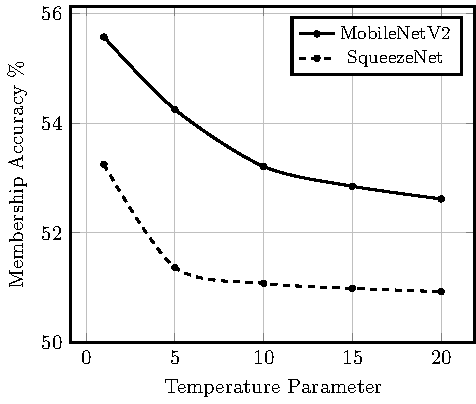
\includegraphics[width=0.6\columnwidth]{figures/efficientArch.pdf}
  \caption{The privacy leakage of off-the-shelf models is reduced by increasing the softmax temperature (CIFAR10 dataset).}
  \label{softmax}
\vspace{-2mm}
\end{figure}

Further, the membership inference accuracy of SqueezeNet and MobileNet can be further reduced close to random guess by increasing the temperature parameter of the softmax function applied to the output.
Increasing the temperature parameter reduces the granularity of the model's output and is given by $F_i(x) = e^{\frac{z_i(x)}{T}}$ / $ \sum_{j}e^{\frac{z_j(x)}{T}}$ where $z(x)$ computes output of the model before the softmax layer.
For the case of SqueezeNet, we are able to reduce the inference accuracy to 50.93\% from 53.07\% while for MobileNet we can reduce the inference accuracy to 52.62\% from 55.57\% as seen in Figure~\ref{softmax}.
This reduction in membership inference accuracy is without any cost of the prediction test accuracy of the model.




\subsubsection{Quantization}\label{quant}

In this section, we evaluate the technique of reducing the precision of both model's parameters and intermediate activations.
Further, we consider the extreme case of binarizing the parameters and activations allowing to evaluate on the most optimized case.
We evaluate on FashionMNIST dataset for two architectures with convolutional and fully connected layers as seen in Table~\ref{fmnist_quantize}.

\begin{table}[!htb]
\begin{center}
\renewcommand\arraystretch{1.5}
\fontsize{6.5pt}{6.5pt}\selectfont
\begin{tabular}{|c|c|c|c|c|}
\hline
\multicolumn{5}{|c|}{\textbf{FashionMNIST}}\\
\hline
\textbf{Architecture} & \textbf{Memory} & \textbf{Train}  & \textbf{Test}  & \textbf{Inference}  \\
 & \textbf{Accuracy} &  \textbf{Footprint} & \textbf{Accuracy} & \textbf{Accuracy}  \\
\hline
\multicolumn{5}{|c|}{Architecture 1}\\
Full & 38.39 MB & 100\% & 92.35\% & \cellcolor{red!25}57.46\%\\
BinaryNet & 1.62 MB & 88.68\% & 86.9\% & \cellcolor{green!25}55.45\%\\
XNOR-Net & 1.62 MB & 87.19\% & 85.68\% & \cellcolor{green!25}51.05\%\\ %1,626,824 parameters
\hline
\multicolumn{5}{|c|}{Architecture 2}\\
Full & 29.83 MB & 99.34\% & 89.88\% & \cellcolor{red!25}54.86\% \\
BinaryNet & 0.93 MB & 97.61\% & 89.60\% & \cellcolor{green!25}54.30\%\\
XNOR-Net & 0.93 MB & 92.67\% & 86.68\% & \cellcolor{green!25}51.74\%\\ %937,000parameters
\hline
\end{tabular}
\end{center}
\caption{Reducing the model precision reduces the inference attack but at the cost of test accuracy.}
\label{fmnist_quantize}
\vspace{-4mm}
\end{table}

In both architectures, we see that computation on  binarized parameters and activations reduces the inference risk by a small value.
However, on replacing the MAC operations with XNOR operations, we observe that the inference risk decreases close to random guess, however, at the cost of prediction test accuracy.
The CIFAR10 results corresponding to the XNOR operations and its privacy comparison with full precision counterpart is indicated in Table~\ref{cifar10quant}.

In summary, we observe that quantization, specifically binarization of parameters and activation along with XNOR computation, provides strong resistance against inference attacks compared to model compression and off-the-shelf architectures.


%\begin{tcolorbox}[enhanced,attach boxed title to top center={yshift=-3mm,yshifttext=-1mm},
%  colback=gray!5!white,colframe=black!75!black,colbacktitle=gray!80!black,
%  title=Security Principle I,fonttitle=\bfseries,
%  boxed title style={size=small,colframe=black!50!black} ]
%Original inputs should not be revealed in the public cloud without proper protection.
%\end{tcolorbox}


\subsection{Summary of Comparison}
\label{eval-summary}

We summarize the properties satisfied by each of the technique in terms of privacy, computation, memory and energy efficiency in Table~\ref{tbl:comparison}.
Here, we mark the attributes which are satisfied with $\cmark$, requires additional hardware optimization as $\smark$ and does not satisfy the property with a $\xmark$.

\begin{table}[!htb]
\begin{center}
\renewcommand\arraystretch{1.5}
\fontsize{6.5pt}{6.5pt}\selectfont
\begin{tabular}{|l||l|l|l|}
\hline
Requirements & Compression & Quantization & Off-the-shelf  \\
\hline
Computation Efficiency & $\smark$  & $\cmark$   & $\xmark$ \\
\hline
Memory Efficiency &  $\smark$ & $\cmark$   & $\cmark$ \\
\hline
Energy Efficiency &  $\smark$   & $\cmark$   & $\xmark$ \\
\hline
Privacy &  $\xmark$   & $\cmark$   & $\smark$ \\
\hline
\end{tabular}
\end{center}
\caption{Only quantization satisfies all the requirements.}
%\caption{Comparison of different optimizations for NNs. $\smark$: additional hardware optimization; $\xmark$: requirement not satisfied; $\cmark$: requirement satisfied.}
\label{tbl:comparison}
\vspace{-4mm}
\end{table}

In order to design NNs for embedded devices, quantization (binarization with XNOR computation) is an attractive design choice which not only satisfies the computation, memory and energy efficiency but also provides high resistance against inference attacks.
On the other hand, model compression without any weight sharing modifications, leaks more training data membership details making it significantly more vulnerable to membership inference attacks. Additionally, it requires hardware support and optimization to achieve better efficiency.
Off-the-shelf architectures, while provide decent privacy, does not satisfy all aspects of efficiency.
Hence, we choose quantization as a NN design for \method\hspace{0.01in} to provide a good three dimensional trade-off between privacy-efficiency-accuracy.


%\pgfplotsset{footnotesize,height=5.5cm,width=0.35\textwidth}
% \pgfplotsset{footnotesize,samples=10}

\begin{figure*}[ht!]
\begin{center}% note that \centering uses less vspace...
\resizebox{2\columnwidth}{!}{%
\begin{tabular}{lllll}


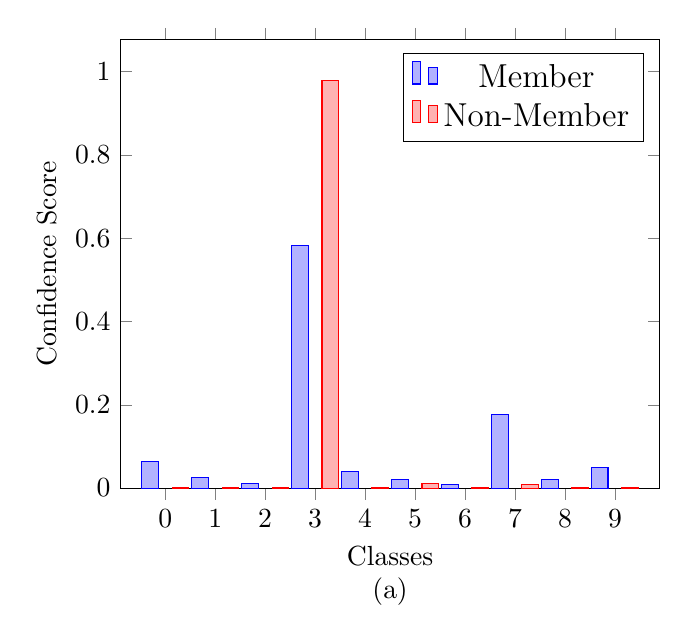
\begin{tikzpicture}
\begin{axis}[title={(a)},
title style={at={(0.5,0)},anchor=north,yshift=-35},
ylabel=Confidence Score,
xlabel=Classes,
legend style={font=\large},
legend pos =  north east,
ybar=5pt,% configures ‘bar shift’
bar width=6pt,
xtick={0,1,2,3,4,5,6,7,8,9},
ymin=0
]

\addplot
coordinates {(0,0.06327114254236221) (1,0.025417674332857132) (2,0.011714407242834568) (3,0.5831579566001892) (4,0.04046289622783661) (5,0.02152826450765133) (6,0.00799587182700634) (7,0.1768314242362976) (8,0.021124042570590973) (9,0.04849636182188988)};
\addplot
coordinates {(0,0.0010145490523427725) (1,0.00030558116850443184) (2,0.0008154626120813191) (3,0.9787409901618958) (4,0.00029880856163799763) (5,0.010064681060612202) (6,0.00022722511494066566) (7,0.007986118085682392) (8,0.00020130971097387373) (9,0.00034515938023105264)};

\legend{Member,Non-Member}
\end{axis}
\end{tikzpicture} &


%
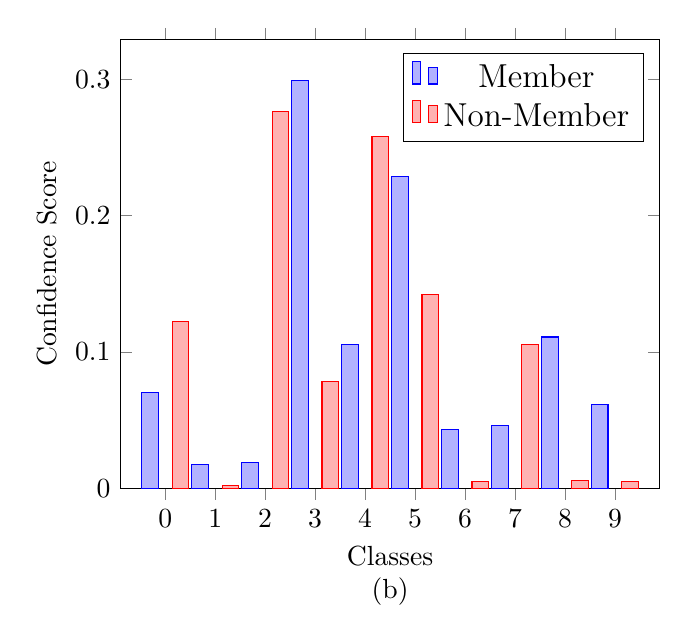
\begin{tikzpicture}
\begin{axis}[title={(b)},
title style={at={(0.5,0)},anchor=north,yshift=-35},
ylabel=Confidence Score,
xlabel=Classes,
xtick={0,1,2,3,4,5,6,7,8,9},
legend style={font=\large},
legend pos =  north east,
ybar=5pt,% configures ‘bar shift’
bar width=6pt,
ymin=0
]

\addplot
coordinates {(0,0.07000309228897095) (1,0.017400363460183144) (2,0.019030457362532616) (3,0.29907193779945374) (4,0.10515590757131577) (5,0.22833536565303802) (6,0.04266407713294029) (7,0.04584269970655441) (8,0.11086355894804001) (9,0.061632607132196426)};
\addplot
coordinates {(0,0.12253900617361069) (1,0.0015809950418770313) (2,0.27642616629600525) (3,0.07850959151983261) (4,0.2582301199436188) (5,0.14231687784194946) (6,0.004606064409017563) (7,0.10550655424594879) (8,0.005763859022408724) (9,0.004520699847489595)};

\legend{Member,Non-Member}
\end{axis}
\end{tikzpicture} &





%
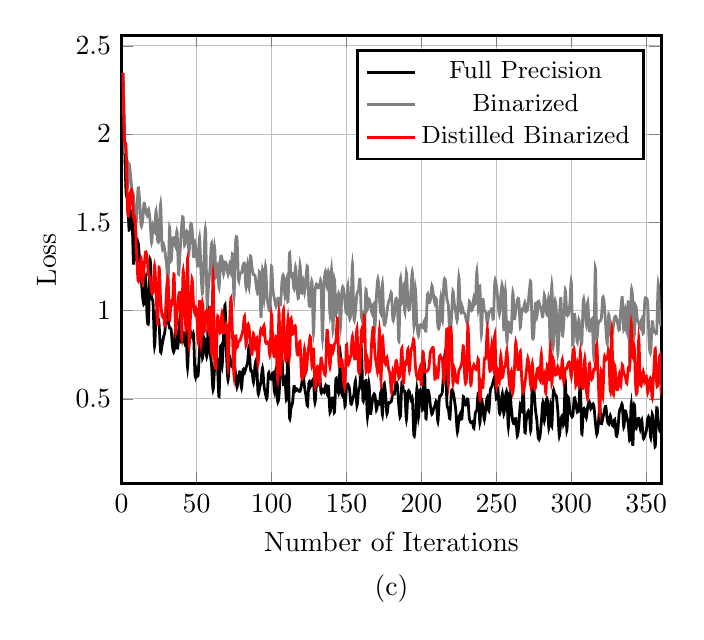
\begin{tikzpicture}
\begin{axis}[title={(c)},
title style={at={(0.5,0)},anchor=north,yshift=-35},
line width=1.0pt,
legend style={font=\small},
legend pos =  north east,
legend entries={Full Precision, Binarized, Distilled Binarized},
ylabel={Loss},
xmin=0,
xmax=360,
xlabel={Number of Iterations},
% extra x ticks={1,10,...,400},
% extra y ticks={0,0.5,...,10},
% extra y tick labels={},
% extra x tick labels={},
% extra x tick style={grid=major},
% extra y tick style={grid=major},
grid=major
]
\addplot[
    color=black,
    solid,
    smooth
    ]
    coordinates {
    ( 1 , 2.302968 )
    ( 2 , 1.939443 )
    ( 3 , 1.667299 )
    ( 4 , 1.652660 )
    ( 5 , 1.455838 )
    ( 6 , 1.559521 )
    ( 7 , 1.526025 )
    ( 8 , 1.260517 )
    ( 9 , 1.503018 )
    ( 10 , 1.285601 )
    ( 11 , 1.384281 )
    ( 12 , 1.286194 )
    ( 13 , 1.191418 )
    ( 14 , 1.079983 )
    ( 15 , 1.039906 )
    ( 16 , 1.188020 )
    ( 17 , 0.963824 )
    ( 18 , 0.943251 )
    ( 19 , 1.289535 )
    ( 20 , 1.082280 )
    ( 21 , 1.037991 )
    ( 22 , 0.799126 )
    ( 23 , 0.983668 )
    ( 24 , 0.966282 )
    ( 25 , 0.922792 )
    ( 26 , 0.765660 )
    ( 27 , 0.803365 )
    ( 28 , 0.850827 )
    ( 29 , 0.893062 )
    ( 30 , 1.063586 )
    ( 31 , 0.948933 )
    ( 32 , 0.901259 )
    ( 33 , 0.895251 )
    ( 34 , 0.794324 )
    ( 35 , 0.769924 )
    ( 36 , 0.899247 )
    ( 37 , 0.787751 )
    ( 38 , 0.831077 )
    ( 39 , 0.962390 )
    ( 40 , 0.821883 )
    ( 41 , 0.863004 )
    ( 42 , 0.818929 )
    ( 43 , 0.880331 )
    ( 44 , 0.676965 )
    ( 45 , 0.891206 )
    ( 46 , 0.876807 )
    ( 47 , 0.854072 )
    ( 48 , 0.860776 )
    ( 49 , 0.631650 )
    ( 50 , 0.662787 )
    ( 51 , 0.630878 )
    ( 52 , 0.778465 )
    ( 53 , 0.900262 )
    ( 54 , 0.731535 )
    ( 55 , 0.845547 )
    ( 56 , 0.785181 )
    ( 57 , 0.748590 )
    ( 58 , 0.986032 )
    ( 59 , 0.774422 )
    ( 60 , 0.691421 )
    ( 61 , 0.551147 )
    ( 62 , 0.668453 )
    ( 63 , 0.759031 )
    ( 64 , 0.673677 )
    ( 65 , 0.512989 )
    ( 66 , 0.796980 )
    ( 67 , 0.681779 )
    ( 68 , 0.851441 )
    ( 69 , 1.030697 )
    ( 70 , 0.751324 )
    ( 71 , 0.606460 )
    ( 72 , 0.733667 )
    ( 73 , 0.701998 )
    ( 74 , 0.680291 )
    ( 75 , 0.707206 )
    ( 76 , 0.645020 )
    ( 77 , 0.566519 )
    ( 78 , 0.622747 )
    ( 79 , 0.651569 )
    ( 80 , 0.560384 )
    ( 81 , 0.663585 )
    ( 82 , 0.648072 )
    ( 83 , 0.676273 )
    ( 84 , 0.701089 )
    ( 85 , 0.797614 )
    ( 86 , 0.665663 )
    ( 87 , 0.657626 )
    ( 88 , 0.592905 )
    ( 89 , 0.687644 )
    ( 90 , 0.712525 )
    ( 91 , 0.533854 )
    ( 92 , 0.557828 )
    ( 93 , 0.599991 )
    ( 94 , 0.673825 )
    ( 95 , 0.575448 )
    ( 96 , 0.526772 )
    ( 97 , 0.505667 )
    ( 98 , 0.643386 )
    ( 99 , 0.620009 )
    ( 100 , 0.610189 )
    ( 101 , 0.647692 )
    ( 102 , 0.539143 )
    ( 103 , 0.667260 )
    ( 104 , 0.489376 )
    ( 105 , 0.518314 )
    ( 106 , 0.676982 )
    ( 107 , 0.727331 )
    ( 108 , 0.581430 )
    ( 109 , 0.618056 )
    ( 110 , 0.500167 )
    ( 111 , 0.785589 )
    ( 112 , 0.399176 )
    ( 113 , 0.447618 )
    ( 114 , 0.475429 )
    ( 115 , 0.570146 )
    ( 116 , 0.544356 )
    ( 117 , 0.555152 )
    ( 118 , 0.546433 )
    ( 119 , 0.542349 )
    ( 120 , 0.577833 )
    ( 121 , 0.639318 )
    ( 122 , 0.567917 )
    ( 123 , 0.517693 )
    ( 124 , 0.460981 )
    ( 125 , 0.593507 )
    ( 126 , 0.570267 )
    ( 127 , 0.597812 )
    ( 128 , 0.598578 )
    ( 129 , 0.478810 )
    ( 130 , 0.586665 )
    ( 131 , 0.579736 )
    ( 132 , 0.659663 )
    ( 133 , 0.538597 )
    ( 134 , 0.549711 )
    ( 135 , 0.537823 )
    ( 136 , 0.572637 )
    ( 137 , 0.534132 )
    ( 138 , 0.570913 )
    ( 139 , 0.422553 )
    ( 140 , 0.488932 )
    ( 141 , 0.504971 )
    ( 142 , 0.423515 )
    ( 143 , 0.614434 )
    ( 144 , 0.564107 )
    ( 145 , 0.541557 )
    ( 146 , 0.744249 )
    ( 147 , 0.522557 )
    ( 148 , 0.606243 )
    ( 149 , 0.458936 )
    ( 150 , 0.558472 )
    ( 151 , 0.581740 )
    ( 152 , 0.556220 )
    ( 153 , 0.470633 )
    ( 154 , 0.493428 )
    ( 155 , 0.524618 )
    ( 156 , 0.601933 )
    ( 157 , 0.460702 )
    ( 158 , 0.542096 )
    ( 159 , 0.583347 )
    ( 160 , 0.778570 )
    ( 161 , 0.497549 )
    ( 162 , 0.533701 )
    ( 163 , 0.603471 )
    ( 164 , 0.397012 )
    ( 165 , 0.583966 )
    ( 166 , 0.417388 )
    ( 167 , 0.471393 )
    ( 168 , 0.520279 )
    ( 169 , 0.520528 )
    ( 170 , 0.437146 )
    ( 171 , 0.482065 )
    ( 172 , 0.469343 )
    ( 173 , 0.539111 )
    ( 174 , 0.408798 )
    ( 175 , 0.585470 )
    ( 176 , 0.532898 )
    ( 177 , 0.415162 )
    ( 178 , 0.476431 )
    ( 179 , 0.477853 )
    ( 180 , 0.486712 )
    ( 181 , 0.538571 )
    ( 182 , 0.526860 )
    ( 183 , 0.590460 )
    ( 184 , 0.575449 )
    ( 185 , 0.451290 )
    ( 186 , 0.401073 )
    ( 187 , 0.596629 )
    ( 188 , 0.545198 )
    ( 189 , 0.532833 )
    ( 190 , 0.382534 )
    ( 191 , 0.532536 )
    ( 192 , 0.539632 )
    ( 193 , 0.492966 )
    ( 194 , 0.496653 )
    ( 195 , 0.291686 )
    ( 196 , 0.359933 )
    ( 197 , 0.558284 )
    ( 198 , 0.393615 )
    ( 199 , 0.546782 )
    ( 200 , 0.507714 )
    ( 201 , 0.441790 )
    ( 202 , 0.694662 )
    ( 203 , 0.387495 )
    ( 204 , 0.539195 )
    ( 205 , 0.534799 )
    ( 206 , 0.460438 )
    ( 207 , 0.412882 )
    ( 208 , 0.439468 )
    ( 209 , 0.461498 )
    ( 210 , 0.484441 )
    ( 211 , 0.371391 )
    ( 212 , 0.505832 )
    ( 213 , 0.518648 )
    ( 214 , 0.544090 )
    ( 215 , 0.680713 )
    ( 216 , 0.751645 )
    ( 217 , 0.478645 )
    ( 218 , 0.442678 )
    ( 219 , 0.387577 )
    ( 220 , 0.538398 )
    ( 221 , 0.543274 )
    ( 222 , 0.495477 )
    ( 223 , 0.428225 )
    ( 224 , 0.311347 )
    ( 225 , 0.386528 )
    ( 226 , 0.415797 )
    ( 227 , 0.386841 )
    ( 228 , 0.512556 )
    ( 229 , 0.467811 )
    ( 230 , 0.469653 )
    ( 231 , 0.497145 )
    ( 232 , 0.386810 )
    ( 233 , 0.365984 )
    ( 234 , 0.370858 )
    ( 235 , 0.334157 )
    ( 236 , 0.421482 )
    ( 237 , 0.437231 )
    ( 238 , 0.533400 )
    ( 239 , 0.363779 )
    ( 240 , 0.499905 )
    ( 241 , 0.448234 )
    ( 242 , 0.381877 )
    ( 243 , 0.457827 )
    ( 244 , 0.508316 )
    ( 245 , 0.432367 )
    ( 246 , 0.550766 )
    ( 247 , 0.567483 )
    ( 248 , 0.600920 )
    ( 249 , 0.619330 )
    ( 250 , 0.501078 )
    ( 251 , 0.563693 )
    ( 252 , 0.420956 )
    ( 253 , 0.452368 )
    ( 254 , 0.529415 )
    ( 255 , 0.413688 )
    ( 256 , 0.507326 )
    ( 257 , 0.534332 )
    ( 258 , 0.340995 )
    ( 259 , 0.533992 )
    ( 260 , 0.445496 )
    ( 261 , 0.371866 )
    ( 262 , 0.357937 )
    ( 263 , 0.387621 )
    ( 264 , 0.290543 )
    ( 265 , 0.351936 )
    ( 266 , 0.467249 )
    ( 267 , 0.429069 )
    ( 268 , 0.564726 )
    ( 269 , 0.309757 )
    ( 270 , 0.382020 )
    ( 271 , 0.423434 )
    ( 272 , 0.425730 )
    ( 273 , 0.322237 )
    ( 274 , 0.597025 )
    ( 275 , 0.560745 )
    ( 276 , 0.445284 )
    ( 277 , 0.378794 )
    ( 278 , 0.276946 )
    ( 279 , 0.282341 )
    ( 280 , 0.366811 )
    ( 281 , 0.478299 )
    ( 282 , 0.375445 )
    ( 283 , 0.480307 )
    ( 284 , 0.493695 )
    ( 285 , 0.336665 )
    ( 286 , 0.462213 )
    ( 287 , 0.346743 )
    ( 288 , 0.541349 )
    ( 289 , 0.522342 )
    ( 290 , 0.514670 )
    ( 291 , 0.430172 )
    ( 292 , 0.289797 )
    ( 293 , 0.371195 )
    ( 294 , 0.405113 )
    ( 295 , 0.357373 )
    ( 296 , 0.603785 )
    ( 297 , 0.321793 )
    ( 298 , 0.506746 )
    ( 299 , 0.432704 )
    ( 300 , 0.405093 )
    ( 301 , 0.403066 )
    ( 302 , 0.504766 )
    ( 303 , 0.473787 )
    ( 304 , 0.425059 )
    ( 305 , 0.450767 )
    ( 306 , 0.582399 )
    ( 307 , 0.300974 )
    ( 308 , 0.433699 )
    ( 309 , 0.439344 )
    ( 310 , 0.394054 )
    ( 311 , 0.458976 )
    ( 312 , 0.482490 )
    ( 313 , 0.442764 )
    ( 314 , 0.467489 )
    ( 315 , 0.462829 )
    ( 316 , 0.372411 )
    ( 317 , 0.298418 )
    ( 318 , 0.353107 )
    ( 319 , 0.452360 )
    ( 320 , 0.359912 )
    ( 321 , 0.388992 )
    ( 322 , 0.428388 )
    ( 323 , 0.456512 )
    ( 324 , 0.380230 )
    ( 325 , 0.357444 )
    ( 326 , 0.403996 )
    ( 327 , 0.361251 )
    ( 328 , 0.344514 )
    ( 329 , 0.381908 )
    ( 330 , 0.289464 )
    ( 331 , 0.320182 )
    ( 332 , 0.425570 )
    ( 333 , 0.448104 )
    ( 334 , 0.466504 )
    ( 335 , 0.340016 )
    ( 336 , 0.430965 )
    ( 337 , 0.396781 )
    ( 338 , 0.356925 )
    ( 339 , 0.267577 )
    ( 340 , 0.468913 )
    ( 341 , 0.233512 )
    ( 342 , 0.466996 )
    ( 343 , 0.332996 )
    ( 344 , 0.367131 )
    ( 345 , 0.389329 )
    ( 346 , 0.330957 )
    ( 347 , 0.378960 )
    ( 348 , 0.278310 )
    ( 349 , 0.290548 )
    ( 350 , 0.316687 )
    ( 351 , 0.388542 )
    ( 352 , 0.388174 )
    ( 353 , 0.279368 )
    ( 354 , 0.412089 )
    ( 355 , 0.335098 )
    ( 356 , 0.229976 )
    ( 357 , 0.449180 )
    ( 358 , 0.374953 )
    ( 359 , 0.321231 )
    ( 360 , 0.348795 )
      };

      \addplot[
          color=gray,
          solid,
          smooth
          ]
          coordinates {
          ( 1 , 2.346761 )
  ( 2 , 1.926266 )
  ( 3 , 1.885543 )
  ( 4 , 1.695635 )
  ( 5 , 1.828619 )
  ( 6 , 1.763135 )
  ( 7 , 1.675170 )
  ( 8 , 1.648822 )
  ( 9 , 1.501599 )
  ( 10 , 1.517566 )
  ( 11 , 1.694481 )
  ( 12 , 1.630272 )
  ( 13 , 1.482632 )
  ( 14 , 1.509774 )
  ( 15 , 1.607969 )
  ( 16 , 1.573090 )
  ( 17 , 1.538904 )
  ( 18 , 1.573854 )
  ( 19 , 1.506782 )
  ( 20 , 1.384800 )
  ( 21 , 1.485137 )
  ( 22 , 1.445732 )
  ( 23 , 1.566089 )
  ( 24 , 1.400355 )
  ( 25 , 1.410617 )
  ( 26 , 1.602641 )
  ( 27 , 1.363793 )
  ( 28 , 1.374451 )
  ( 29 , 1.327962 )
  ( 30 , 1.259157 )
  ( 31 , 1.158507 )
  ( 32 , 1.471694 )
  ( 33 , 1.281064 )
  ( 34 , 1.395380 )
  ( 35 , 1.413245 )
  ( 36 , 1.364599 )
  ( 37 , 1.446778 )
  ( 38 , 1.205966 )
  ( 39 , 1.332203 )
  ( 40 , 1.474646 )
  ( 41 , 1.530147 )
  ( 42 , 1.370293 )
  ( 43 , 1.436183 )
  ( 44 , 1.444681 )
  ( 45 , 1.332167 )
  ( 46 , 1.484209 )
  ( 47 , 1.465831 )
  ( 48 , 1.305787 )
  ( 49 , 1.380785 )
  ( 50 , 1.305335 )
  ( 51 , 1.252715 )
  ( 52 , 1.414409 )
  ( 53 , 1.208195 )
  ( 54 , 1.097216 )
  ( 55 , 1.304714 )
  ( 56 , 1.456459 )
  ( 57 , 1.040485 )
  ( 58 , 1.141915 )
  ( 59 , 1.240699 )
  ( 60 , 1.379954 )
  ( 61 , 1.174325 )
  ( 62 , 1.360094 )
  ( 63 , 1.193203 )
  ( 64 , 1.246328 )
  ( 65 , 1.128607 )
  ( 66 , 1.297393 )
  ( 67 , 1.293353 )
  ( 68 , 1.207303 )
  ( 69 , 1.274779 )
  ( 70 , 1.260201 )
  ( 71 , 1.205472 )
  ( 72 , 1.257582 )
  ( 73 , 1.209281 )
  ( 74 , 1.320339 )
  ( 75 , 1.081225 )
  ( 76 , 1.379258 )
  ( 77 , 1.403371 )
  ( 78 , 1.173059 )
  ( 79 , 1.210906 )
  ( 80 , 1.212522 )
  ( 81 , 1.256900 )
  ( 82 , 1.261412 )
  ( 83 , 1.132829 )
  ( 84 , 1.261608 )
  ( 85 , 1.130152 )
  ( 86 , 1.307679 )
  ( 87 , 1.242157 )
  ( 88 , 1.203381 )
  ( 89 , 1.197875 )
  ( 90 , 1.127777 )
  ( 91 , 1.099596 )
  ( 92 , 1.218491 )
  ( 93 , 0.959279 )
  ( 94 , 1.230520 )
  ( 95 , 1.063139 )
  ( 96 , 1.248715 )
  ( 97 , 1.083069 )
  ( 98 , 1.019647 )
  ( 99 , 1.012220 )
  ( 100 , 1.250834 )
  ( 101 , 1.113485 )
  ( 102 , 1.065619 )
  ( 103 , 1.023666 )
  ( 104 , 1.063910 )
  ( 105 , 1.067258 )
  ( 106 , 1.032276 )
  ( 107 , 1.165910 )
  ( 108 , 1.197135 )
  ( 109 , 1.079468 )
  ( 110 , 1.176466 )
  ( 111 , 1.049984 )
  ( 112 , 1.325067 )
  ( 113 , 1.198396 )
  ( 114 , 1.209702 )
  ( 115 , 1.122866 )
  ( 116 , 1.246204 )
  ( 117 , 1.130638 )
  ( 118 , 1.070367 )
  ( 119 , 1.258520 )
  ( 120 , 1.100373 )
  ( 121 , 1.169035 )
  ( 122 , 1.103153 )
  ( 123 , 1.187527 )
  ( 124 , 1.249404 )
  ( 125 , 1.039255 )
  ( 126 , 1.043600 )
  ( 127 , 1.163061 )
  ( 128 , 0.866229 )
  ( 129 , 1.100545 )
  ( 130 , 1.150101 )
  ( 131 , 1.129426 )
  ( 132 , 1.129657 )
  ( 133 , 1.159651 )
  ( 134 , 0.838983 )
  ( 135 , 1.136622 )
  ( 136 , 1.221408 )
  ( 137 , 1.139824 )
  ( 138 , 1.213746 )
  ( 139 , 0.979337 )
  ( 140 , 1.232616 )
  ( 141 , 0.885131 )
  ( 142 , 1.174824 )
  ( 143 , 0.979129 )
  ( 144 , 1.055910 )
  ( 145 , 1.090147 )
  ( 146 , 0.904567 )
  ( 147 , 1.113498 )
  ( 148 , 1.125462 )
  ( 149 , 1.049405 )
  ( 150 , 0.985949 )
  ( 151 , 1.139380 )
  ( 152 , 0.959967 )
  ( 153 , 1.000041 )
  ( 154 , 1.263282 )
  ( 155 , 0.956478 )
  ( 156 , 0.995327 )
  ( 157 , 1.096886 )
  ( 158 , 1.111590 )
  ( 159 , 1.176757 )
  ( 160 , 0.962864 )
  ( 161 , 0.977689 )
  ( 162 , 0.922844 )
  ( 163 , 1.120963 )
  ( 164 , 1.009984 )
  ( 165 , 1.063984 )
  ( 166 , 1.032832 )
  ( 167 , 0.987173 )
  ( 168 , 1.035523 )
  ( 169 , 0.903309 )
  ( 170 , 1.083587 )
  ( 171 , 1.178625 )
  ( 172 , 1.068447 )
  ( 173 , 0.984077 )
  ( 174 , 1.152232 )
  ( 175 , 0.932497 )
  ( 176 , 0.932060 )
  ( 177 , 0.994724 )
  ( 178 , 1.047627 )
  ( 179 , 1.068406 )
  ( 180 , 1.097718 )
  ( 181 , 0.946308 )
  ( 182 , 0.981098 )
  ( 183 , 1.067997 )
  ( 184 , 1.027874 )
  ( 185 , 0.826300 )
  ( 186 , 1.179658 )
  ( 187 , 1.052969 )
  ( 188 , 1.142715 )
  ( 189 , 0.991129 )
  ( 190 , 1.213003 )
  ( 191 , 1.045486 )
  ( 192 , 1.006147 )
  ( 193 , 1.109902 )
  ( 194 , 1.212793 )
  ( 195 , 0.912005 )
  ( 196 , 1.123085 )
  ( 197 , 0.926187 )
  ( 198 , 0.858419 )
  ( 199 , 0.916872 )
  ( 200 , 0.915458 )
  ( 201 , 0.904451 )
  ( 202 , 0.942618 )
  ( 203 , 0.883013 )
  ( 204 , 1.090961 )
  ( 205 , 1.045205 )
  ( 206 , 1.059832 )
  ( 207 , 1.141301 )
  ( 208 , 1.089335 )
  ( 209 , 1.039749 )
  ( 210 , 1.063170 )
  ( 211 , 0.912232 )
  ( 212 , 0.915569 )
  ( 213 , 1.075158 )
  ( 214 , 0.940946 )
  ( 215 , 1.157747 )
  ( 216 , 1.170259 )
  ( 217 , 1.066205 )
  ( 218 , 1.024397 )
  ( 219 , 0.852790 )
  ( 220 , 0.950637 )
  ( 221 , 1.110507 )
  ( 222 , 1.036702 )
  ( 223 , 0.984222 )
  ( 224 , 0.952827 )
  ( 225 , 1.188724 )
  ( 226 , 1.000404 )
  ( 227 , 1.028348 )
  ( 228 , 0.988035 )
  ( 229 , 0.983033 )
  ( 230 , 0.942389 )
  ( 231 , 0.935704 )
  ( 232 , 1.051824 )
  ( 233 , 1.005647 )
  ( 234 , 1.006882 )
  ( 235 , 1.072922 )
  ( 236 , 1.043638 )
  ( 237 , 1.221575 )
  ( 238 , 1.003483 )
  ( 239 , 1.138196 )
  ( 240 , 0.862098 )
  ( 241 , 1.062384 )
  ( 242 , 0.999307 )
  ( 243 , 0.991120 )
  ( 244 , 0.926649 )
  ( 245 , 0.986342 )
  ( 246 , 0.992192 )
  ( 247 , 1.010563 )
  ( 248 , 0.952089 )
  ( 249 , 1.165234 )
  ( 250 , 1.141195 )
  ( 251 , 1.059924 )
  ( 252 , 0.980622 )
  ( 253 , 1.091556 )
  ( 254 , 1.136913 )
  ( 255 , 0.883962 )
  ( 256 , 1.111804 )
  ( 257 , 0.826448 )
  ( 258 , 0.934091 )
  ( 259 , 0.895227 )
  ( 260 , 0.889213 )
  ( 261 , 1.103202 )
  ( 262 , 0.953661 )
  ( 263 , 1.005441 )
  ( 264 , 1.058801 )
  ( 265 , 1.057636 )
  ( 266 , 0.903979 )
  ( 267 , 1.003013 )
  ( 268 , 1.001371 )
  ( 269 , 1.045060 )
  ( 270 , 0.995644 )
  ( 271 , 1.017072 )
  ( 272 , 1.109493 )
  ( 273 , 1.156392 )
  ( 274 , 0.859848 )
  ( 275 , 0.867010 )
  ( 276 , 1.039820 )
  ( 277 , 0.963619 )
  ( 278 , 1.051263 )
  ( 279 , 1.029461 )
  ( 280 , 1.002586 )
  ( 281 , 0.965037 )
  ( 282 , 1.089420 )
  ( 283 , 1.019706 )
  ( 284 , 0.973446 )
  ( 285 , 1.068585 )
  ( 286 , 0.790222 )
  ( 287 , 1.146344 )
  ( 288 , 0.802443 )
  ( 289 , 1.046202 )
  ( 290 , 0.997245 )
  ( 291 , 0.754709 )
  ( 292 , 0.945580 )
  ( 293 , 1.069640 )
  ( 294 , 0.858742 )
  ( 295 , 0.934347 )
  ( 296 , 1.114184 )
  ( 297 , 0.985928 )
  ( 298 , 0.977279 )
  ( 299 , 1.034217 )
  ( 300 , 1.159927 )
  ( 301 , 0.804602 )
  ( 302 , 0.978465 )
  ( 303 , 0.916436 )
  ( 304 , 0.819233 )
  ( 305 , 0.947365 )
  ( 306 , 0.873999 )
  ( 307 , 0.814669 )
  ( 308 , 1.060480 )
  ( 309 , 1.009367 )
  ( 310 , 0.923004 )
  ( 311 , 1.046344 )
  ( 312 , 0.884677 )
  ( 313 , 0.931433 )
  ( 314 , 0.941696 )
  ( 315 , 0.756139 )
  ( 316 , 1.241746 )
  ( 317 , 0.852658 )
  ( 318 , 0.924763 )
  ( 319 , 0.942495 )
  ( 320 , 0.954869 )
  ( 321 , 1.075119 )
  ( 322 , 1.036582 )
  ( 323 , 0.906247 )
  ( 324 , 0.812499 )
  ( 325 , 0.977565 )
  ( 326 , 0.870054 )
  ( 327 , 0.857418 )
  ( 328 , 0.904272 )
  ( 329 , 0.964146 )
  ( 330 , 0.960810 )
  ( 331 , 0.922262 )
  ( 332 , 0.889789 )
  ( 333 , 1.004996 )
  ( 334 , 1.073944 )
  ( 335 , 0.891395 )
  ( 336 , 1.000604 )
  ( 337 , 0.882347 )
  ( 338 , 1.048631 )
  ( 339 , 0.699180 )
  ( 340 , 1.102788 )
  ( 341 , 1.062422 )
  ( 342 , 0.861747 )
  ( 343 , 1.025133 )
  ( 344 , 0.951212 )
  ( 345 , 0.927888 )
  ( 346 , 0.904762 )
  ( 347 , 0.950766 )
  ( 348 , 0.868892 )
  ( 349 , 1.051545 )
  ( 350 , 1.070194 )
  ( 351 , 1.035250 )
  ( 352 , 0.803139 )
  ( 353 , 0.765967 )
  ( 354 , 0.936454 )
  ( 355 , 0.882868 )
  ( 356 , 0.877807 )
  ( 357 , 0.886292 )
  ( 358 , 1.150183 )
  ( 359 , 0.951342 )
  ( 360 , 0.913005 )
            };

  \addplot[
      color=red,
      solid,
      smooth
      ]
      coordinates {
      ( 1 , 2.346761 )
      ( 1 , 2.289508 )
      ( 2 , 1.958497 )
      ( 3 , 1.921034 )
      ( 4 , 1.561351 )
      ( 5 , 1.560222 )
      ( 6 , 1.672546 )
      ( 7 , 1.671921 )
      ( 8 , 1.527745 )
      ( 9 , 1.516091 )
      ( 10 , 1.320806 )
      ( 11 , 1.168530 )
      ( 12 , 1.210074 )
      ( 13 , 1.297815 )
      ( 14 , 1.161482 )
      ( 15 , 1.246961 )
      ( 16 , 1.331731 )
      ( 17 , 1.299713 )
      ( 18 , 1.200435 )
      ( 19 , 1.183215 )
      ( 20 , 1.105063 )
      ( 21 , 1.109861 )
      ( 22 , 1.254844 )
      ( 23 , 1.108233 )
      ( 24 , 0.924076 )
      ( 25 , 1.244691 )
      ( 26 , 1.063551 )
      ( 27 , 0.970651 )
      ( 28 , 0.976295 )
      ( 29 , 0.913169 )
      ( 30 , 1.119265 )
      ( 31 , 1.173765 )
      ( 32 , 0.947561 )
      ( 33 , 1.054491 )
      ( 34 , 1.046588 )
      ( 35 , 1.206818 )
      ( 36 , 0.882458 )
      ( 37 , 0.983017 )
      ( 38 , 1.080579 )
      ( 39 , 1.086890 )
      ( 40 , 0.842886 )
      ( 41 , 1.221012 )
      ( 42 , 1.075716 )
      ( 43 , 0.899074 )
      ( 44 , 1.293818 )
      ( 45 , 0.811225 )
      ( 46 , 0.981191 )
      ( 47 , 1.177047 )
      ( 48 , 1.032480 )
      ( 49 , 0.981890 )
      ( 50 , 1.005604 )
      ( 51 , 0.828696 )
      ( 52 , 1.057695 )
      ( 53 , 0.824240 )
      ( 54 , 1.040227 )
      ( 55 , 0.879299 )
      ( 56 , 0.971962 )
      ( 57 , 0.997197 )
      ( 58 , 0.886545 )
      ( 59 , 1.017593 )
      ( 60 , 0.762022 )
      ( 61 , 1.199266 )
      ( 62 , 0.736034 )
      ( 63 , 0.687340 )
      ( 64 , 0.962291 )
      ( 65 , 0.905756 )
      ( 66 , 0.875405 )
      ( 67 , 0.986668 )
      ( 68 , 0.885548 )
      ( 69 , 0.877220 )
      ( 70 , 0.914856 )
      ( 71 , 0.682138 )
      ( 72 , 0.919164 )
      ( 73 , 1.070877 )
      ( 74 , 0.855854 )
      ( 75 , 0.627857 )
      ( 76 , 0.856239 )
      ( 77 , 0.792077 )
      ( 78 , 0.823261 )
      ( 79 , 0.830847 )
      ( 80 , 0.857799 )
      ( 81 , 0.892394 )
      ( 82 , 0.966335 )
      ( 83 , 0.803680 )
      ( 84 , 0.914873 )
      ( 85 , 0.908078 )
      ( 86 , 0.798237 )
      ( 87 , 0.752717 )
      ( 88 , 0.869953 )
      ( 89 , 0.796312 )
      ( 90 , 0.844140 )
      ( 91 , 0.699578 )
      ( 92 , 0.830843 )
      ( 93 , 0.896852 )
      ( 94 , 0.871961 )
      ( 95 , 0.915021 )
      ( 96 , 0.821148 )
      ( 97 , 0.817516 )
      ( 98 , 0.820520 )
      ( 99 , 0.750622 )
      ( 100 , 0.976288 )
      ( 101 , 0.791571 )
      ( 102 , 0.738218 )
      ( 103 , 0.854439 )
      ( 104 , 0.610627 )
      ( 105 , 0.990846 )
      ( 106 , 0.649290 )
      ( 107 , 0.813209 )
      ( 108 , 1.002776 )
      ( 109 , 0.739490 )
      ( 110 , 0.742654 )
      ( 111 , 0.952149 )
      ( 112 , 0.742725 )
      ( 113 , 0.953895 )
      ( 114 , 0.866470 )
      ( 115 , 0.899595 )
      ( 116 , 0.905452 )
      ( 117 , 0.761735 )
      ( 118 , 0.759309 )
      ( 119 , 0.824847 )
      ( 120 , 0.632895 )
      ( 121 , 0.629622 )
      ( 122 , 0.782615 )
      ( 123 , 0.652874 )
      ( 124 , 0.728099 )
      ( 125 , 0.806889 )
      ( 126 , 0.848280 )
      ( 127 , 0.685887 )
      ( 128 , 0.781918 )
      ( 129 , 0.568329 )
      ( 130 , 0.653542 )
      ( 131 , 0.681325 )
      ( 132 , 0.587069 )
      ( 133 , 0.728819 )
      ( 134 , 0.688508 )
      ( 135 , 0.655295 )
      ( 136 , 0.647998 )
      ( 137 , 0.887438 )
      ( 138 , 0.804118 )
      ( 139 , 0.681075 )
      ( 140 , 0.801215 )
      ( 141 , 0.765510 )
      ( 142 , 0.810749 )
      ( 143 , 0.832472 )
      ( 144 , 0.954358 )
      ( 145 , 0.698934 )
      ( 146 , 0.696781 )
      ( 147 , 0.720781 )
      ( 148 , 0.611648 )
      ( 149 , 0.570984 )
      ( 150 , 0.805634 )
      ( 151 , 0.698532 )
      ( 152 , 0.715090 )
      ( 153 , 0.752225 )
      ( 154 , 0.854783 )
      ( 155 , 0.743349 )
      ( 156 , 0.737030 )
      ( 157 , 0.898713 )
      ( 158 , 0.668182 )
      ( 159 , 0.672265 )
      ( 160 , 0.889392 )
      ( 161 , 0.825691 )
      ( 162 , 0.970438 )
      ( 163 , 0.662543 )
      ( 164 , 0.723655 )
      ( 165 , 0.652735 )
      ( 166 , 0.684006 )
      ( 167 , 0.844469 )
      ( 168 , 0.903263 )
      ( 169 , 0.756717 )
      ( 170 , 0.695948 )
      ( 171 , 0.658278 )
      ( 172 , 0.890274 )
      ( 173 , 0.604330 )
      ( 174 , 0.846531 )
      ( 175 , 0.740486 )
      ( 176 , 0.697799 )
      ( 177 , 0.732877 )
      ( 178 , 0.674738 )
      ( 179 , 0.642503 )
      ( 180 , 0.539443 )
      ( 181 , 0.657330 )
      ( 182 , 0.605968 )
      ( 183 , 0.715463 )
      ( 184 , 0.682130 )
      ( 185 , 0.617121 )
      ( 186 , 0.661775 )
      ( 187 , 0.788635 )
      ( 188 , 0.588687 )
      ( 189 , 0.700439 )
      ( 190 , 0.697120 )
      ( 191 , 0.781461 )
      ( 192 , 0.660160 )
      ( 193 , 0.770010 )
      ( 194 , 0.800414 )
      ( 195 , 0.835379 )
      ( 196 , 0.684457 )
      ( 197 , 0.623300 )
      ( 198 , 0.611837 )
      ( 199 , 0.672864 )
      ( 200 , 0.579889 )
      ( 201 , 0.766305 )
      ( 202 , 0.661602 )
      ( 203 , 0.654130 )
      ( 204 , 0.659236 )
      ( 205 , 0.676831 )
      ( 206 , 0.763144 )
      ( 207 , 0.783112 )
      ( 208 , 0.779393 )
      ( 209 , 0.611283 )
      ( 210 , 0.660481 )
      ( 211 , 0.622174 )
      ( 212 , 0.739116 )
      ( 213 , 0.736537 )
      ( 214 , 0.717488 )
      ( 215 , 0.603474 )
      ( 216 , 0.720956 )
      ( 217 , 0.895162 )
      ( 218 , 0.583987 )
      ( 219 , 0.885873 )
      ( 220 , 0.865381 )
      ( 221 , 0.591229 )
      ( 222 , 0.669389 )
      ( 223 , 0.612504 )
      ( 224 , 0.592590 )
      ( 225 , 0.660891 )
      ( 226 , 0.677134 )
      ( 227 , 0.708002 )
      ( 228 , 0.798415 )
      ( 229 , 0.613641 )
      ( 230 , 0.610063 )
      ( 231 , 0.912058 )
      ( 232 , 0.711359 )
      ( 233 , 0.578273 )
      ( 234 , 0.661869 )
      ( 235 , 0.692462 )
      ( 236 , 0.670032 )
      ( 237 , 0.670372 )
      ( 238 , 0.722965 )
      ( 239 , 0.490983 )
      ( 240 , 0.599413 )
      ( 241 , 0.564405 )
      ( 242 , 0.720429 )
      ( 243 , 0.738146 )
      ( 244 , 0.895175 )
      ( 245 , 0.716247 )
      ( 246 , 0.657736 )
      ( 247 , 0.809308 )
      ( 248 , 0.673177 )
      ( 249 , 0.861484 )
      ( 250 , 0.572226 )
      ( 251 , 0.659255 )
      ( 252 , 0.596616 )
      ( 253 , 0.746455 )
      ( 254 , 0.621354 )
      ( 255 , 0.668629 )
      ( 256 , 0.692351 )
      ( 257 , 0.772648 )
      ( 258 , 0.658080 )
      ( 259 , 0.568799 )
      ( 260 , 0.655683 )
      ( 261 , 0.536369 )
      ( 262 , 0.655911 )
      ( 263 , 0.821214 )
      ( 264 , 0.690711 )
      ( 265 , 0.666788 )
      ( 266 , 0.769021 )
      ( 267 , 0.603920 )
      ( 268 , 0.538827 )
      ( 269 , 0.586855 )
      ( 270 , 0.653802 )
      ( 271 , 0.729698 )
      ( 272 , 0.662506 )
      ( 273 , 0.573307 )
      ( 274 , 0.698765 )
      ( 275 , 0.571538 )
      ( 276 , 0.560311 )
      ( 277 , 0.653228 )
      ( 278 , 0.674414 )
      ( 279 , 0.609833 )
      ( 280 , 0.754565 )
      ( 281 , 0.590132 )
      ( 282 , 0.637046 )
      ( 283 , 0.533268 )
      ( 284 , 0.690426 )
      ( 285 , 0.608395 )
      ( 286 , 0.782570 )
      ( 287 , 0.586600 )
      ( 288 , 0.720135 )
      ( 289 , 0.644524 )
      ( 290 , 0.636831 )
      ( 291 , 0.682296 )
      ( 292 , 0.644609 )
      ( 293 , 0.619640 )
      ( 294 , 0.721622 )
      ( 295 , 0.595761 )
      ( 296 , 0.669771 )
      ( 297 , 0.672078 )
      ( 298 , 0.702717 )
      ( 299 , 0.700702 )
      ( 300 , 0.623715 )
      ( 301 , 0.752632 )
      ( 302 , 0.772183 )
      ( 303 , 0.574867 )
      ( 304 , 0.694724 )
      ( 305 , 0.579246 )
      ( 306 , 0.763784 )
      ( 307 , 0.584890 )
      ( 308 , 0.568738 )
      ( 309 , 0.728641 )
      ( 310 , 0.555155 )
      ( 311 , 0.508444 )
      ( 312 , 0.696937 )
      ( 313 , 0.616997 )
      ( 314 , 0.615176 )
      ( 315 , 0.667652 )
      ( 316 , 0.675299 )
      ( 317 , 0.810867 )
      ( 318 , 0.603052 )
      ( 319 , 0.418517 )
      ( 320 , 0.652455 )
      ( 321 , 0.513917 )
      ( 322 , 0.730091 )
      ( 323 , 0.720278 )
      ( 324 , 0.729959 )
      ( 325 , 0.768966 )
      ( 326 , 0.547639 )
      ( 327 , 0.893457 )
      ( 328 , 0.526425 )
      ( 329 , 0.687370 )
      ( 330 , 0.572277 )
      ( 331 , 0.553026 )
      ( 332 , 0.636406 )
      ( 333 , 0.578816 )
      ( 334 , 0.692453 )
      ( 335 , 0.641644 )
      ( 336 , 0.629935 )
      ( 337 , 0.588312 )
      ( 338 , 0.677901 )
      ( 339 , 0.682241 )
      ( 340 , 0.924726 )
      ( 341 , 0.736128 )
      ( 342 , 0.794371 )
      ( 343 , 0.559741 )
      ( 344 , 0.550659 )
      ( 345 , 0.842112 )
      ( 346 , 0.594323 )
      ( 347 , 0.587956 )
      ( 348 , 0.653175 )
      ( 349 , 0.598934 )
      ( 350 , 0.627735 )
      ( 351 , 0.535564 )
      ( 352 , 0.593137 )
      ( 353 , 0.614303 )
      ( 354 , 0.503203 )
      ( 355 , 0.654863 )
      ( 356 , 0.783821 )
      ( 357 , 0.581702 )
      ( 358 , 0.599832 )
      ( 359 , 0.742905 )
      ( 360 , 0.518803 )
        };

\end{axis}
\end{tikzpicture}
\end{tabular}
}
\caption{(a) The confidence scores are distinguishable between train and test data records in undefended models trained making them vulnerable to membership inference attacks. (b) \method\hspace{0.02in} models have indistinguishable confidence scores. (c) The loss trajectories in Phase I is higher than Phase II indicating the improvement in accuracy.}
\label{fig:loss}
\end{center}
\end{figure*}


\subsection{Evaluating Phase I}
\label{evalPh1}

In Phase I of \method, we quantize the model and replace the MACs with cheap XNOR operations.
We observe that the inference attack accuracy decreases significantly for all the three architecture close to random guess ($\sim$50\%).
Specifically, the inference accuracy decreases from 56.69\% to 51.76\% for NiN, 60.40\% to 51.40\% for AlexNet and 58.70\% to 52.65\% for VGGNet.


\begin{table}[!htb]
\begin{center}
\renewcommand\arraystretch{1.5}
\fontsize{6.5pt}{6.5pt}\selectfont
\begin{tabular}{|c|c|c|c|c|}
\hline
\multicolumn{5}{|c|}{\textbf{CIFAR10}} \\
\hline
\multicolumn{2}{|c|}{\textbf{Architecture}} & \textbf{Train}  & \textbf{Test}  & \textbf{Inference}  \\
 \multicolumn{2}{|c|}{} & \textbf{Accuracy} & \textbf{Accuracy} & \textbf{Accuracy}  \\
\hline
\multirow{2}{*}{NiN} & Full Precision & 98.16\% & 86.16\% & \cellcolor{red!25}56.69\% \\
& Binary Precision & 81.93\% & 78.74\% & \cellcolor{green!25}51.76\% \\
\hline
\multirow{2}{*}{AlexNet} & Full Precision & 97.86\% & 80.34\% & \cellcolor{red!25}60.40\% \\
& Binary Precision & 68.62\% & 66.8\% & \cellcolor{green!25}51.40\% \\
\hline
\multirow{2}{*}{VGG13} & Full Precision & 99.58\% & 88.95\% & \cellcolor{red!25}58.70\%\\
& Binary Precision & 79.67\% & 74.64\% & \cellcolor{green!25}52.65\%\\
\hline
\end{tabular}
\end{center}
\caption{Reducing the precision of models lowers the membership privacy leakage but at the cost of accuracy.}
%through membership inference attacks
\label{cifar10quant}
\end{table}


However, since Phase I only optimizes the network for privacy and efficiency, the resultant model shows poor utility (accuracy).
We observe a significant loss in test accuracy for all the three models: around 8\% accuracy drop from 86.16\% to 78.74\% for NiN; 14\% accuracy drop from 80.34\% to 66.8\% for AlexNet; 14\% for VGG model from 88.95\% to 74.64\%.
In order to restore the accuracy, we use knowledge distillation as described in Phase II of the \method\hspace{0.02in} framework.

The privacy provided by quantized NN is due to the decrease in overfitting, empirically measured using the difference between the train and test accuracy.
The leakage in inference accuracy is attributed to the higher overfitting in models as well as memorization of the training data information in the form of the parameters, which are specifically tuned to achieve high performance on the train data~\cite{10.1145/3133956.3134077,236216,DBLP:journals/corr/abs-1812-00910}.
This is attributed to the reduction in learning capacity of the model on quantizing the parameters which lowers the sensitive training data information memorized by the parameters on lowering the precision.
Further, the quantization acts as a noise to strongly regularize the model~\cite{NIPS2016_6573}.
At the same time, this optimization provides high degree of efficiency to be executed on low powered embedded devices.

\subsection{Evaluating Phase II}
\label{evalPh2}

The objective of Phase II of \method\hspace{0.02in} is to enhance the accuracy of the quantized model with XNOR computations which depicts high inference attack resistance and efficiency.
In Phase II, we use the teacher-student model (described in Section~\ref{design}) to train the quantized student model being guided using the output predictions of the full precision teacher model.
Here, Phase II is heterogeneous, i.e, we are flexible to choose any full precision teacher model which can provide high accuracy on the considered dataset (Table~\ref{kd}).
Here, we consider pre-trained state of the art architectures\footnote{https://github.com/huyvnphan/PyTorch\_CIFAR10}: DenseNet169 and ResNet50, along with the full precision versions of NiN, Alexnet and VGGNet.
The standalone test accuracy of the DenseNet169 and ResNet50 architectures are 92.84\% and 92.12\% respectively with inference accuracy around to 55\% while the full precision accuracies for NiN, AlexNet and VGGNet are given in Table~\ref{cifar10quant}.


\begin{table}[!htb]
\begin{center}
\renewcommand\arraystretch{1.5}
\fontsize{6.5pt}{6.5pt}\selectfont
\begin{tabular}{|c|c|c|c|c|c|}
\hline
\textbf{Teacher} & \textbf{Student} & \textbf{Train}  & \textbf{Test}  & \textbf{Inference}  \\
&  & \textbf{Accuracy} & \textbf{Accuracy} & \textbf{Accuracy}  \\
\hline
\multicolumn{5}{|c|}{Standalone Models}\\
\hline
Binary NiN & None & 81.93\% & 78.74\% & 51.76\% \\
Binary AlexNet & None & 68.62\% & 66.8\% & 51.40\% \\
Binary VGG13 & None & 79.67\% & 74.64\% & 52.65\%\\
\hline
\multicolumn{5}{|c|}{Homogeneous Architecture Distillation}\\
\hline
NiN & Binary NiN & 90.49\% & 83.52\% & 53.90\% \\
AlexNet & Binary AlexNet & 76.79\% & 73.5\% & 51.85\% \\
VGG13 & Binary VGG13 & 89.45\% & 81.58\% & 54.98\%\\
\hline
\multicolumn{5}{|c|}{Heterogeneous Architecture Distillation}\\
\hline
DenseNet169 & NiN & 92.84\% & 83.71\% & 54.95\%\\
DenseNet169 & AlexNet & 81.87\% & 76.23\% & 53.51\%\\
DenseNet169 & VGG13 & 93.45\% & 85.8\% & 54.17\%\\
\hline
ResNet50 & NiN & 91.74\% & 83.77\% & 54.53\% \\
ResNet50 & AlexNet & 80.12\% & 74.92\% & 53.12\%\\
ResNet50 & VGG13 & 94.23\% & 86.52\% & 54.46\%\\
\hline
\end{tabular}
\end{center}
\caption{Phase II of \method\hspace{0.02in} improves the accuracy of the private-efficient model from Phase I.}
\label{kd}
\vspace{-0.3in}
\end{table}


The first set of experiments combine the same full precision model architectures with the quantized model versions, i.e, full precision NiN with Binarized NiN (homogeneous knowledge distillation).
Here, we see that there is 5\% increase in test accuracy (from 78.74\% to 83.52\%) for NiN with an increase of 2\% in inference attack.
Similarly, there is an increase of 7\% test accuracy for AlexNet with a very minimal privacy leakage increase of 0.45\%; and increase of 7\% test accuracy at the cost of 2\% inference attack accuracy for VGGNet.
For heterogeneous knowledge distillation, i.e, combining other architectures (DenseNet169 and ResNet50) with the quantized models from Phase I, we see that the increase in test accuracy is only minimally higher than the homogeneous models for NiN and AlexNet but a significantly higher increase in the inference attack accuracy.
However, in case of VGGNet, we observe an increase of 4\% additional test accuracy compared to homogeneous knowledge distillation with a minimal decrease in the inference test accuracy.
In Phase II, increase in test accuracy is accompanied with a small but acceptable increase in the inference attack accuracy indicating a privacy-utility trade-off.
Hence, the choice of using homogeneous or heterogeneous knowledge distillation is specific to the architecture and the privacy-utility requirements of the application.
Compared to the full precision counterparts, we observe that the distilled models show an accuracy degradation of only 3\% for NiN(86.66\% to 83.77\%), 4\% for AlexNet (80.34\% to 76.23\%) and 2\% for VGGNet (88.95\% to 86.52\%).

The \method\hspace{0.02in} framework results in models which make the output confidence of the train and test data records similar reducing the inference attack accuracy (Figure~\ref{fig:loss}).
Further, the knowledge distillation enables to lower the loss of the model compared to the model trained in Phase I resulting in higher test accuracy as seen in Figure~\ref{fig:loss} (c).
However, the loss trajectory is still higher than the full precision version indicating the test accuracy degradation of the proposed framework and a privacy-utility trade-off.

\subsection{Comparison with Prior Defences}
\label{eval-defences}

The defences proposed in literature can be categorized into (a) regularization based train-time defences and (b) post-training inference time defence.
Adversarial Regularization, Differential Privacy and other standard regularization techniques such as L2 and Dropout modify the training of the neural network.
Our proposed training framework exploits is part of category (a) where we modify the training of the machine learning model in order to provide acceptable levels of privacy and accuracy.

\begin{figure}[ht!]
\begin{center}% note that \centering uses less vspace...
\resizebox{\columnwidth}{!}{%
\begin{tikzpicture}
    \begin{axis}[
        footnotesize,
        % set the `width' of the plot to the maximum length ...
        width=\textwidth,
        % ... and use half this length for the `height'
        height=0.5\textwidth,
        % use `data' for the positioning of the `xticks' ...
        xtick=data,
        % ... and use table data for labeling the `xticks'
        xticklabels from table={comparedef.txt}{n},
        % add extra ticks "at the empty entries to add the vertical lines
        extra x ticks={5,11,17,23},
        % this ticks shouldn't be labeled ...
        extra x tick labels={},
        % ... but grid lines should be drawn without the tick lines
        extra x tick style={
            grid=major,
            major tick length=0pt,
        },
        ymin=0,
        ymax=105,
        xlabel={Number of Layers},
        ylabel={Accuracy \%},
        % because of the category labels, shift the `xlabel' a bit down
        xlabel style={
            yshift=-4ex,
        },
        legend style={at={(0.5,-0.15)},anchor=north,legend columns=-1},
        % adjust `bar width' so it fits your needs ...
        bar width=8pt,
        % ... and with that you also have to adjust the x limits
        enlarge x limits={abs=1},
        % set `clip mode' to `individual' so the category labels aren't clipped away
        clip mode=individual,
    ]

    % plot the "red" ybars
        \addplot [
            ybar,
            draw=red,
            pattern color=red,
            pattern=dots,
        ] table [
            % use just the `coordindex' as x coordinate,
            % the correct labeling is done with `xticklabels from table'
            x expr=\coordindex,
            y=pFA,
        ] {comparedef.txt};

    % plot the "blue" ybars
        \addplot [
            ybar,
            draw=blue,
            pattern color=blue,
            pattern=north east lines,
        ] table [
            x expr=\coordindex,
            y=pFB,
        ] {comparedef.txt};

    \addplot[draw=black,mark=*,thick,smooth] coordinates {(0,56.69) (1,51.92) (2,54.09) (3,52.90)};
    \addplot[draw=black,mark=*,thick,smooth] coordinates {(5,60.40) (6,51.83) (7,52.81) (8,51.85)};
    \addplot[draw=black,mark=*,thick,smooth] coordinates {(10,58.70) (11,53.33) (12,52.90) (13,53.17)};
    \addplot[draw=black,dashed,thick,smooth] coordinates {(0,50)(1,50)(2,50)(3,50)(4,50)(5,50)(6,50)(7,50)(8,50)(9,50)(10,50)(11,50)(12,50)(13,50)};


    % add the category labels
        \begin{scope}[
            % because the reference point will be the lower axis line the
            % labels have to be moved a bit more down to don't overlap with
            % the `xticklabels'
            every label/.append style={
                label distance=2ex,
            },
        ]
            \node [label=below:NiN] at (axis cs:1.5,\pgfkeysvalueof{/pgfplots/ymin}) {};
            \node [label=below:AlexNet] at (axis cs:6.5,\pgfkeysvalueof{/pgfplots/ymin}) {};
            \node [label=below:VGG] at (axis cs:11.5,\pgfkeysvalueof{/pgfplots/ymin}) {};

        \end{scope}
    \legend{Train Accuracy,Test Accuracy,Inference Accuracy}
    \end{axis}
\end{tikzpicture}
}
\caption{\underline{Comparison with prior defences.} Models trained using \method\hspace{0.02in} training methodology are comparable to prior state of the art defences: Adversarial Regularization and Differential Privacy, in terms of test accuracy and inference accuracy while additionally ensuring efficiency.}
\label{fig:compare}
\end{center}
\end{figure}


The comparison of models trained using \method\hspace{0.02in} is shown in Figure~\ref{fig:compare}.
Models trained using \method\hspace{0.02in} are comparable in test accuracy and resisting membership inference leakage to Adversarial Regularization and Differential Privacy.
The inference accuracy for NiN is 52.90\% (\method) compared to 54.09\% (DP) and 51.92\% (AdvReg) and test accuracy of 83.52\% (\method) compared to 85.11\% (DP) and 83.66\% (AdvReg).
For AlexNet, the inference accuracy is 51.85\% (\method) compared to 52.81\% (DP) and 51.83\% (AdvReg) and test accuracy of 73.5\% (\method) compared to 79.27\% (DP) and 71.02\% (AdvReg).
For VGGNet, the inference accuracy is 53.17\% (\method) compared to 52.90\% (DP) and 53.33\% (AdvReg) and test accuracy of 85.8\% (\method) compared to 84.91\% (DP) and 85.19\% (AdvReg).
In addition, our proposed models additionally provide efficiency guarantees enabling them to be used for embedded systems.

\noindent\textbf{Comparison with MemGuard.} MemGuard~\cite{10.1145/3319535.3363201} is a post-training defence, where the defender adds carefully crafted noise to the target model's output observations to ensure the misclassification of the adversary's attack classifier network.
The defence assumes the adversary's attack model is an ML classifier vulnerable to adversarial examples.
However, this post-training approach can be used in addition to the models trained using the \method\hspace{0.02in} framework assuming the adversary uses shadow model attack.
Our attack does not rely on a "shadow" models but rather relies on output posterior to perform the attack.
Hence, within the threat model considered, the defence is not valid for comparison.

\section{Related Work}\label{related}


\noindent\textbf{Machine Learning Privacy.} Data privacy in Machine Learning addresses different inference attacks such as membership inference~\cite{salem2018ml,shokri2017membership}.
While these works have been evaluated in a blackbox setting, privacy leakage through inference attacks have been studied in the context of whitebox setting~\cite{DBLP:journals/corr/abs-1812-00910}.
Further, generative model have been shown to be vulnerable to membership inference attacks~\cite{LOGANMembershipInferenceAttacksAgainstGenerativeModels} and distributed setting such as in federated learning have also been exploited~\cite{melis2019exploiting,DBLP:journals/corr/abs-1812-00910}.
These privacy leakage in machine learning models have been mainly attributed to the memorization of training data by the models~\cite{236216,10.1145/3133956.3134077}.
In order to mitigate against inference attacks several defences have been explored such as Differential Privacy~\cite{Abadi:2016:DLD:2976749.2978318}, simple and adversarial regularization~\cite{DBLP:conf/ccs/NasrSH18,salem2018ml} which aim to generalize the model and alternatively, adding noise to the predictions to increase error~\cite{10.1145/3319535.3363201}.
Alternatively, confidential computing aims to privately and efficiently compute machine learning models using secure multiparty computation~\cite{235489}.


\noindent\textbf{Efficient Deep Learning.} Hardware-Software Co-Design is crucial to accelerate the performance of NNs on hardware.
Hardware accelerators reuse weights and intermediate computation enable significant performance improvement~\cite{10.1109/ISCA.2016.30}.
Algorithmic optimizations have explored model compression through pruning~\cite{Han:2015:LBW:2969239.2969366} and reducing the precision of the model parameters and activations to binary~\cite{NIPS2016_6573}, ternary~\cite{Li2016TernaryWN} and generic quantization~\cite{Hubara:2017:QNN:3122009.3242044}.
Binarization enables to replace multiplication with simple boolean logic improving the overall performance~\cite{rastegari2016xnornet}.
Alternatively, hardware optimizations have enabled to design NN accelerators for low precision NNs for further efficiency~\cite{Umuroglu2017FINNAF}.
Further, specialized architectures designed for low memory footprint have also been extensively used for low powered devices such as mobile phones and micro-controllers~\cite{DBLP:journals/corr/IandolaMAHDK16,conf/cvpr/SandlerHZZC18}. 

\section{Conclusions}\label{conclusions}

On device processing of sensitive data using NNs on embedded systems requires a careful analysis of privacy, efficiency and accuracy of the algorithms which is currently lacking in literature.
In this work, we propose a two phase \method\hspace{0.02in} framework to design private, efficient and accurate NNs for execution on low powered embedded devices.
We quantify the privacy leakage using membership inference attacks where the adversary aims to infer whether a given data record was used in the model's training data.
We first provide a comprehensive privacy and efficiency analysis of state of the art algorithms for improving efficiency: model compression (pruning), quantization and efficient off-the-shelf architectures.
We show that model compression leaks more information compared to the original (uncompressed) model while off-the-shelf architectures do not provide the best efficiency guarantees.
Based on these observations, we use quantization as a design choice which shows high resistance against inference attacks while satisfying all the efficiency requirements.
While Phase I of \method\hspace{0.02in} optimizes for privacy and efficiency, in Phase II, we improve the accuracy of the resultant model using knowledge transfer from full precision models.
Our extensive evaluations of state of the art architectures on CIFAR10 dataset indicates that models trained using the proposed framework provides high resistance against membership inference attacks (comparable to other state of the art defences) with high efficiency.



%{\footnotesize
%\bibliographystyle{IEEEtranS}
%\bibliography{paper.bib}
%}

\bibliographystyle{ACM-Reference-Format}
\bibliography{paper}

%\section*{Appendix}

\subsection{Impact of Model Compression}

We evaluate the privacy leakage of model compression on two other datasets: Location and Purchase100.

\noindent\textbf{Purchase100.} This dataset is a privacy sensitive dataset capturing the purchase preferences of online customers taken from the authors of~\cite{shokri2017membership}.
The data records have 600 binary features and each record is classified into one of 100 classes identifying each user's purchase.
For this dataset, we use a fully connected architecture with the nodes in each layers as [1024,512,256,128,100].

\noindent\textbf{Location.} This dataset is a privacy sensitive dataset capturing user's location "check-ins" taken from the authors of~\cite{shokri2017membership} where each record has 446 binary features which is mapped to one of 30 classes each representing a location. For this dataset we use a fully connected architecture with hyperparameters as [512,256,128,30].

\begin{figure}[!htb]
    \centering
    \begin{minipage}[b]{1\linewidth}
    \centering
    \subfigure[Impact of Pruning on Location (left) and Purchase (right)]{
    \label{fig:mem_soft_label}
    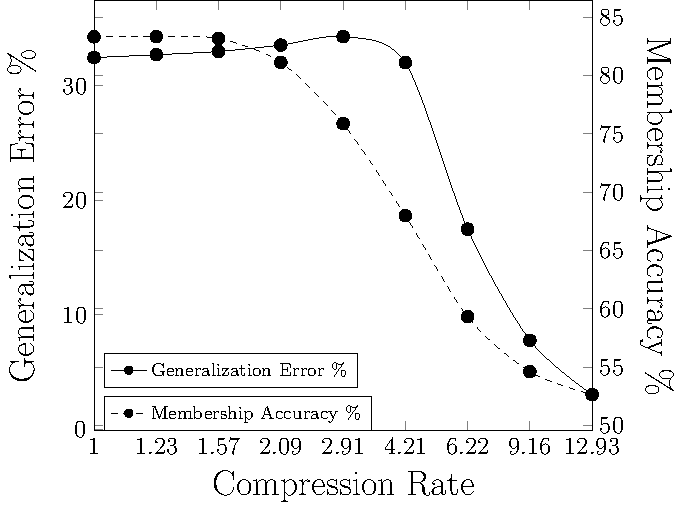
\includegraphics[width=0.5\linewidth]{figures/location_prune.pdf}
    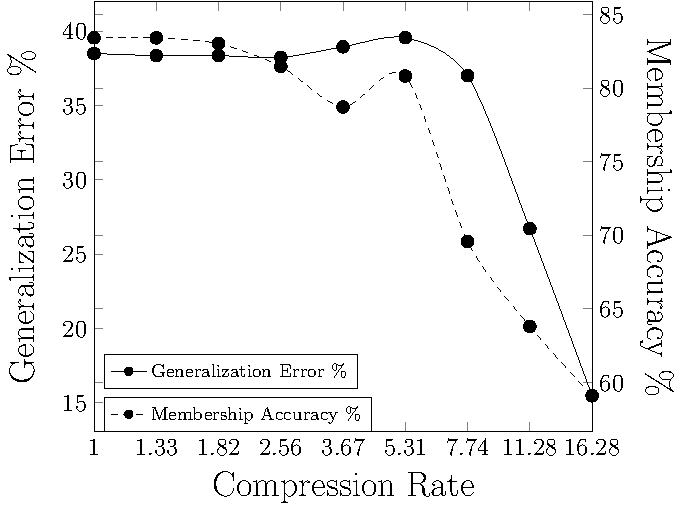
\includegraphics[width=0.5\linewidth]{figures/purchase_prune.pdf}
    }

    \subfigure[Impact of Retraining on Location (left) and Purchase (right)]{
    \label{fig:nonmem_soft_label}
    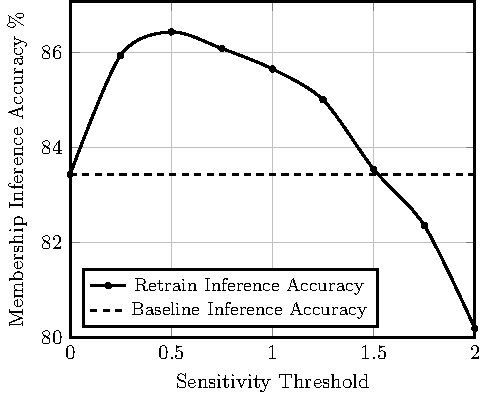
\includegraphics[width=0.5\linewidth]{figures/location_retrain.pdf}
    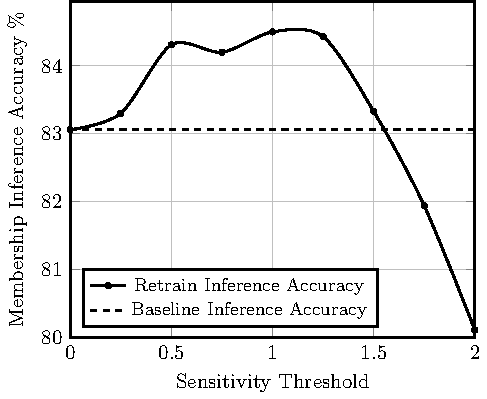
\includegraphics[width=0.5\linewidth]{figures/purchase_retrain.pdf}
    }

    \subfigure[Mitigating Leakage via Weight sharing on Location (left) and Purchase (right)]{
   	\label{fig:mem_soft_label}
    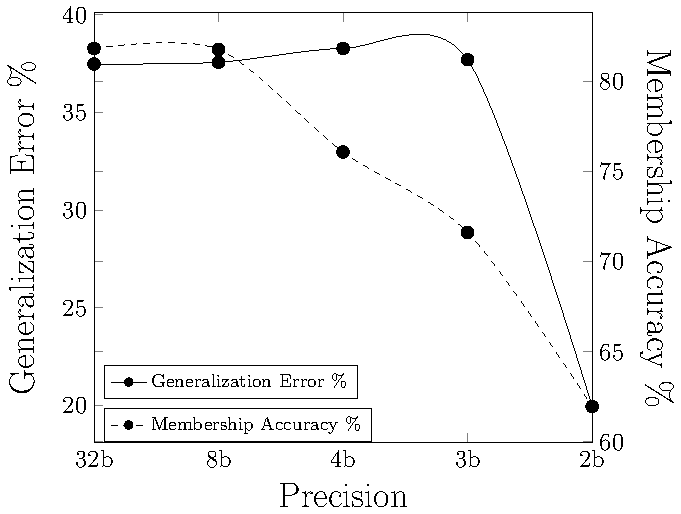
\includegraphics[width=0.5\linewidth]{figures/location_wtsharing.pdf}
    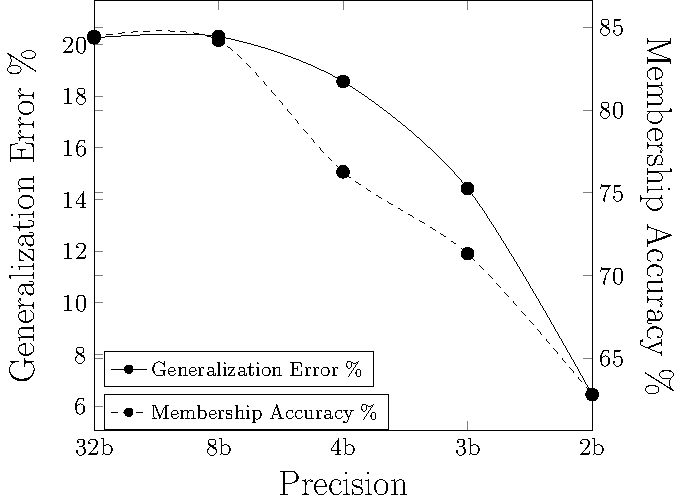
\includegraphics[width=0.5\linewidth]{figures/purchase_wtsharing.pdf}
    }

    \end{minipage}
    \caption{We extend the analysis of privacy leakage due to model compression on two additional datasets.}
    \label{fig:NIAcause}
\end{figure}



\end{document}
\endinput
